\provideboolean{Slides}
\setboolean{Slides}{false}


\ifthenelse{\boolean{inBook}}{
  \newcommand{\bdkhouseholdFull}{Chapter 1, Household Surveys and Probabilistic Questions}
  \newcommand{\bdkhouseholdShort}{Chapter 1}
}{
  \newcommand{\bdkhouseholdFull}{\cite{bdk2021household}}
  \newcommand{\bdkhouseholdShort}{\cite{bdk2021household}}
}

% \setboolean{inBook}{false}
\ifthenelse{\boolean{inBook}}{
  \newcommand{\dmwinflationexpectationFull}{Chapter 7,  Inflation Expectations}
  \newcommand{\dmwinflationexpectationShort}{Chapter 7}
}{
  \newcommand{\dmwinflationexpectationFull}{\cite{dmw2022inflationexpectation}}
  \newcommand{\dmwinflationexpectationShort}{\cite{dmw2022inflationexpectation}}
}


% \setboolean{inBook}{false}
\ifthenelse{\boolean{inBook}}{
  \newcommand{\kpshousingexpectationFull}{Chapter 8,  Housing Market Expectations}
  \newcommand{\kpshousingexpectationShort}{Chapter 8}
}{
  \newcommand{\kpshousingexpectationFull}{\cite{kps2022housingexpectation}}
  \newcommand{\kpshousingexpectationShort}{\cite{kps2022housingexpectation}}
}


\ifthenelse{\boolean{inBook}}{
  \newcommand{\bvbayesianlearningFull}{Chapter  25, Bayesian Learning}
  \newcommand{\bvbayesianlearningShort}{Chapter 25}
}{
  \newcommand{\bvbayesianlearningFull}{\cite{bv2022bayesianlearning}}
  \newcommand{\bvbayesianlearningShort}{\cite{bv2022bayesianlearning}}
}

\newcommand{\thankstext}{Thanks to the participants in the \textit{Handbook of Economic Expectations} Conference for insightful comments, and the editors for comments that substantially improved the paper.  Thanks also to Sebastian Benthall, Francesco Bianchi, Jennifer Manning, and Adrian Monninger for feedback on earlier drafts, and special thanks to Mridul Seth for help in using the \texttt{\href{https://ndlib.readthedocs.io}{NDLib}} and \texttt{\href{https://networkx.org/}{NetworkX}} python libraries to produce our \href{https://econ-ark.org/materials/epiexp?launch}{SIR Model Notebook}.}
\begin{verbatimwrite}{./abstract.tex}
  `Epidemiological' models of belief formation put social interactions at their core; such models are the principal kind of tool used by scholars who are not economists to study the dynamics of beliefs in populations.  We survey the literature in which economists attempting to model the consequences of beliefs about the future -- `expectations' -- have employed a full-fledged epidemiological approach to explore an economic question.  We draw connections to related work on `contagion,' narrative economics, news/rumor spreading, and the spread of internet memes. A main theme of the paper is that a number of independent developments have recently converged to make epidemiological expectations (`EE') modeling more feasible and appealing than in the past.
\end{verbatimwrite}

\ifthenelse{\boolean{inBook}}{
  \begin{frontmatter}%

    \chapter[Chapter Title]{Epidemiological \\ Expectations\footnote{\thankstext}}\label{chap1}

    \author[1]{Christopher Carroll}
    \author[1]{Tao Wang}
    \address[1]{\orgname{Johns Hopkins University}, \orgdiv{Department of Economics}, \\ Corresponding: \email{twang80@jhu.edu}}

    % \authormark{First Author, Second Author and Third Author}
    \titlemark{Part Title}
    \chaptermark{Epidemiological Expectations}

    \MaxmMiniTocnum{A.1}{3.3.3}{}

    \minitoc

    \makechaptertitle
    \begin{keywords}[Keywords:]
      Economic Expectations \sep Epidemiological Expectations \sep Social interactions \sep Social dynamics \sep Information diffusion \sep Economic Narratives
    \end{keywords}
    \begin{keywords}[JEL Codes:]
      D84, D91, E71, G41,
    \end{keywords}
    \hypertarget{abstract}{}
    \begin{abstract}[Abstract]
        `Epidemiological' models of belief formation put social interactions at their core; such models are the principal kind of tool used by scholars who are not economists to study the dynamics of beliefs in populations.  We survey the literature in which economists attempting to model the consequences of beliefs about the future -- `expectations' -- have employed a full-fledged epidemiological approach to explore an economic question.  We draw connections to related work on `contagion,' narrative economics, news/rumor spreading, and the spread of internet memes. A main theme of the paper is that a number of independent developments have recently converged to make epidemiological expectations (`EE') modeling more feasible and appealing than in the past.

    \end{abstract}
    \pagebreak
  }{%else not in book
    \author{Christopher D. Carroll\authNum \\
      \\
      Tao Wang\authNum}

    \title{Epidemiological Expectations}
    \renewcommand{\forcedate}{March 18, 2022}
    \keywords{Economic Expectations,  Epidemiological Expectations,  Social interactions,  Social dynamics,  Information diffusion,  Economic Narratives}
    \jelclass{D84, D91, E71, G41}
    \maketitle
    \hypertarget{abstract}{}
    \begin{abstract}
        `Epidemiological' models of belief formation put social interactions at their core; such models are the principal kind of tool used by scholars who are not economists to study the dynamics of beliefs in populations.  We survey the literature in which economists attempting to model the consequences of beliefs about the future -- `expectations' -- have employed a full-fledged epidemiological approach to explore an economic question.  We draw connections to related work on `contagion,' narrative economics, news/rumor spreading, and the spread of internet memes. A main theme of the paper is that a number of independent developments have recently converged to make epidemiological expectations (`EE') modeling more feasible and appealing than in the past.

    \end{abstract}
    \ifdvi % skip the links because they do not work inside the html
    \else
    \vspace{0.5in}
    \newcommand{\owner}{llorracc}
    \newcommand{\REMARK}{\href{https://github.com/econ-ark/REMARK}{REMARK}}
    \begin{small}
      \parbox{0.9\textwidth}{
        \begin{center}
          \begin{tabbing}
            \texttt{~~~\REMARK:~} \= \= \texttt{\url{https://econ-ark.org/materials/epiexp}} \\
            \texttt{Dashboard:~} \> \> \texttt{\href{https://econ-ark.org/materials/epiexp?launch}{Click `Launch Dashboard' Button}} \\
            \texttt{~~~~~html:~} \> \> \texttt{\href{https://\owner.github.io/EpiExp}{https://\owner.github.io/EpiExp/}} \\ % Owner is defined in Resources/owner.tex
            \texttt{~Book~PDF:~} \> \> \texttt{\href{https://github.com/\owner/EpiExp/blob/master/docs/EpiExp-Book.pdf}{EpiExp-Book.pdf}} \\
            \texttt{~NBER~PDF:~} \> \> \texttt{\href{https://github.com/\owner/EpiExp/blob/master/docs/EpiExp-NBER.pdf}{EpiExp-NBER.pdf}} \\

            \texttt{~~~Slides:~} \> \> \texttt{\href{https://github.com/\owner/EpiExp/blob/master/docs/EpiExp-Slides.pdf}{EpiExp-Slides.pdf}} \\
            \texttt{~~~GitHub:~} \> \> \texttt{\href{https://github.com/\owner/EpiExp}{https://github.com/\owner/EpiExp}} \\
          \end{tabbing}
        \end{center}
      }
    \end{small}
    \fi

    \begin{authorsinfo}
      \name{Contact: \href{mailto:ccarroll@jhu.edu}{\texttt{ccarroll@jhu.edu}}, Department of Economics, 590 Wyman Hall, Johns Hopkins University, Baltimore, MD 21218, \url{https://www.econ2.jhu.edu/people/ccarroll}, and National Bureau of Economic Research; \href{mailto:twang80@jhu.edu}{\texttt{twang80@jhu.edu}}, Department of Economics, 590 Wyman Hall, Johns Hopkins University, Baltimore, MD 21218}
    \end{authorsinfo}

    \begin{center}
      \begin{minipage}{0.9\textwidth}
        {\footnotesize \thankstext \normalsize}
      \end{minipage}
    \end{center}
    \ifthenelse{\boolean{Web}}{
      \par\noindent\rule{\textwidth}{0.4pt}
    }{}
    \titlepagefinish
    \ifthenelse{\boolean{Web}}{}{ % Web version puts this in frame
      \renewcommand{\contentsname}{}
      \tableofcontents
    }
    \small
    \renewcommand{\listtablename}{\normalsize Tables}
    \renewcommand{\listfigurename}{\normalsize Figures}
    \listoffigures
    % \end{minipage}

    \medskip\medskip
    % \begin{minipage}{0.9\textwidth}
    \listoftables
    % \end{minipage}
    \normalsize
    \ifthenelse{\boolean{Web}}{
      \par\noindent\rule{\textwidth}{0.4pt}
    }{\pagebreak}
    \ifthenelse{\boolean{Web}}{
      \par\noindent\rule{\textwidth}{0.4pt}
    }{}
  }

  \setcounter{page}{0}\pagenumbering{arabic}

  \begin{verbatimwrite}{./Slides/QuoteArrow1969}%%%Slides
    \begin{quote}\ifthenelse{\boolean{Slides}}{\footnotesize}{}
      \textit{While mass media play a major role in alerting individuals to the possibility of an innovation, it seems to be personal contact that is most relevant in leading to its adoption. Thus, the diffusion of an innovation becomes a process formally akin to the spread of an infectious disease.}

      % \source{
      \medskip
      \indent -- \href{https://github.com/iworld1991/EpiExp/blob/master/Literature/arrow_classificatory_1969.pdf}{\cite{arrow_classificatory_1969}}
      % }
    \end{quote}
  \end{verbatimwrite} %%%Slides
    \begin{quote}\ifthenelse{\boolean{Slides}}{\footnotesize}{}
    \textit{While mass media play a major role in alerting individuals to the possibility of an innovation, it seems to be personal contact that is most relevant in leading to its adoption. Thus, the diffusion of an innovation becomes a process formally akin to the spread of an infectious disease.}

    \medskip
    \indent -- %\IfPrivate{\href{https://github.com/iworld1991/EpiExp/blob/master/Literature/arrow_classificatory_1969.pdf}{\cite{arrow_classificatory_1969}}}{\cite{arrow_classificatory_1969}}
      \cite{arrow_classificatory_1969}
  \end{quote}
 %%%Slides

  \begin{verbatimwrite}{./Slides/QuoteSimon1984}%%%Slides
    \begin{quote}\ifthenelse{\boolean{Slides}}{\footnotesize}{}
      \textit{A very natural next step for economics is to maintain expectations in	the strategic position they have come to occupy, but to build an empirically validated theory of how attention is in fact directed within a social system, and how expectations are, in fact, formed.}

      % \source{
      \medskip
      \indent -- \href{https://econpapers.repec.org/RePEc:eee:jeborg:v:5:y:1984:i:1:p:35-55}{\cite{simon_behavioral_1984}}
      % }
    \end{quote}
  \end{verbatimwrite} %%%Slides
    \begin{quote}\ifthenelse{\boolean{Slides}}{\footnotesize}{}
    \textit{A very natural next step for economics is to maintain expectations in	the strategic position they have come to occupy, but to build an empirically validated theory of how attention is in fact directed within a social system, and how expectations are, in fact, formed.}
    \medskip
    \indent -- \href{https://econpapers.repec.org/RePEc:eee:jeborg:v:5:y:1984:i:1:p:35-55}{\cite{simon_behavioral_1984}}
  \end{quote}
 %%%Slides

  \begin{verbatimwrite}{./Slides/QuoteShiller2017}%%%Slides
    \begin{quote}\ifthenelse{\boolean{Slides}}{\footnotesize}{}
      \textit{If we want to know why an unusually large economic event happened, we need to list the seemingly unrelated narratives that all happened to be going viral at around the same time and affecting the economy in the same direction.}

      % \source{
      \medskip
      \indent -- \href{https://www.amazon.com/dp/B07VZWLRM8/ref=cm_sw_em_r_mt_dp_BT5KE0VTHQX6DJ35FD9C}{\cite{shiller2017narrative}}
      % }
    \end{quote}
  \end{verbatimwrite} %%%Slides
      \begin{quote}\ifthenelse{\boolean{Slides}}{\footnotesize}{}
      \textit{If we want to know why an unusually large economic event happened, we need to list the seemingly unrelated narratives that all happened to be going viral at around the same time and affecting the economy in the same direction.}

      % \source{
      \medskip
      \indent -- \href{https://www.amazon.com/dp/B07VZWLRM8/ref=cm_sw_em_r_mt_dp_BT5KE0VTHQX6DJ35FD9C}{\cite{shiller2017narrative}}
      % }
    \end{quote}
  
 %%%Slides

  \begin{verbatimwrite}{./Slides/QuoteInception2010}%%%Slides
    \begin{quote}\ifthenelse{\boolean{Slides}}{\footnotesize}{}
      \textit{An idea is like a virus. Resilient. Highly contagious. And even the smallest seed of an idea can grow.}   --Cobb

      % \source{
      \medskip \indent --
      The movie \textit{Inception} [\citeyear{Inception2010}]
      % } % Tao: Fix citation
    \end{quote}
  \end{verbatimwrite} %%%Slides
    \begin{quote}\ifthenelse{\boolean{Slides}}{\footnotesize}{}
    \textit{An idea is like a virus. Resilient. Highly contagious. And even the smallest seed of an idea can grow.}   --Cobb
    \medskip \indent --
    The movie \textit{Inception} [\citeyear{Inception2010}]
  \end{quote}
 %%%Slides

  \ifthenelse{\boolean{inBook}}{
  \end{frontmatter}%
}{}

\section{Introduction}
\label{chap1:sec1}

It is a commonplace, in academia and popular culture, that ideas spread like diseases: they can be ``infectious'' or ``go viral.''  The proposition is hardly new; as \cite{shiller2017narrative} points out, it can be found at least as far back as \cite{humeenquiry}, whose ideas thoroughly infected the work of his friend \cite{smithwealth}.\footnote{See \cite{rasmussen2017infidel}.} Indeed, in fields other than economics, debates are rarely about whether social interactions are fundamental; they are about which particular models of social communication are most suitable for understanding the spread of which kinds of ideas.

``Expectations'' are just a category of ideas.  So upon being told that expectations play a critical role in structural economic modeling, a scholar who was not an economist might suppose that epidemiological approaches would be a standard part of the economist's toolkit for modeling expectations --- unless there were good reason to believe that economic ideas are immune to social influence.  But evidence for social transmission of economic ideas is plentiful -- see Section~\ref{subsec:microEvidence}.

Still, it would not be accurate to say that an `epidemiological expectations' (`EE') approach is a standard way of constructing formal models of economic phenomena -- a conventional off-the-shelf alternative, say, to a `rational expectations' (`RE') approach, the `Rational Inattention' (`RI') approach advocated by~\cite{sims2003implications}, the `diagnostic expectations' model of~\cite{bordalo2018diagnostic}, or a number of bounded rationality approaches (e.g.,~\cite{gabaix2020behavioral} or \cite{ilut2020economic}).

This is perhaps because nowhere has any focused attempt been made to define what would constitute an EE treatment of an economic question.\ifthenelse{\boolean{inBook}}{}{\footnote{A methodology in cultural economics called `the epidemiological approach' seeks to identify cultural variations in behavior the same way epidemiologists sometimes identify disease risks: By a person's place of origin, or other observable exogenous traits that might be markers of cultural attitudes.  Since this approach does not aim to study the transmission of expectations by social interactions, we see little danger of its being confused with what we define as EE modeling.}}  For the purposes of this survey, we will think of a full-fledged EE treatment as incorporating the following elements:
\begin{verbatimwrite}{./Slides/FullFledgedEE}
  \begin{quote}\normalfont
    \begin{enumerate}
    \item \textbf{a mechanism:} \ifthenelse{\boolean{Slides}}{math by which idea(s) transmitted}{An explicit and rigorous mathematical description of a process by which ideas are transmitted between agents  ...}
    \item \textbf{implying expectational dynamics:} \ifthenelse{\boolean{Slides}}{
        ... that yields observable $\mathbb{E}$ dynamics ...
      }
      {... that generates observable expectation dynamics at the level of individuals or populations~...}
    \item \textbf{with economic consequences:} \ifthenelse{\boolean{Slides}}{... those $\mathbb{E} \Rightarrow$ an economic outcome}{
        ... and those expectations have knock-on implications for an observable outcome (often, prices, quantities, or market values) that is the primary subject of the economic analysis.}
    \end{enumerate}
  \end{quote}
\end{verbatimwrite}
  \begin{quote}\normalfont
    \begin{enumerate}
    \item \textbf{a mechanism:} \ifthenelse{\boolean{Slides}}{math by which idea(s) transmitted}{An explicit and rigorous mathematical description of a process by which ideas are communicated between agents  ...}
    \item \textbf{implying expectational dynamics:} \ifthenelse{\boolean{Slides}}{
        ... that yields observable $\mathbb{E}$ dynamics ...
      }
      {... that generates observable expectation dynamics at the level of individuals or populations~...}
    \item \textbf{with economic consequences:} \ifthenelse{\boolean{Slides}}{... those $\mathbb{E} \Rightarrow$ an economic outcome}{
        ... and those expectations have knock-on implications for an observable outcome (often, prices, quantities, or market values) that is the primary subject of the economic analysis.}
    \end{enumerate}
  \end{quote}


\ifthenelse{\boolean{inBook}}{}{These criteria whittle down a vast number of invocations, or partial treatments, of the proposition that ideas spread through social interaction, to the surprisingly small number of papers on which we primarily focus here.  (The last criterion allows us to neglect enormous literatures on public opinion, politics, musical tastes, internet memes, and other topics).}

We have identified three fields in economics -- technological diffusion (section ~\ref{subsec:techDiffusion}), asset pricing (section~\ref{subsec:assetprice}), and macroeconomics (section~\ref{subsec:macroExp}) -- with sets of papers that satisfy all these criteria, even if in some cases the work has not mainly been thought of as `epidemiological' until now.\ifthenelse{\boolean{inBook}}{}{\footnote{Ironically, these literatures have developed largely in isolation from each other, judging at least by the almost complete independence of the citation networks (see our figure~\ref{fig:graph_mixer}). The only paper that is cited by all three literatures is the foundational paper by \cite{kermack_contribution_1927}.}}  In addition, we survey the proliferating evidence that social interactions drive expectations and corresponding behaviors (section~\ref{subsec:microEvidence}); draw connections between the EE approach and a separate literature on financial contagion (section~\ref{subsec:Contagion}); and present selected examples from the research outside of economics that might be particularly interesting for economists (section~\ref{subsec:nonecon}).\ifthenelse{\boolean{inBook}}{}{\footnote{Since the outbreak of the COVID-19 pandemic, a large literature has sprung up in which economists have directly modeled COVID itself as a disease, or modeled the economic consequences of the disease; this work of course does not meet our criteria, but some of it -- e.g. \cite{gourieroux2020time} -- contains interesting techniques for modeling the spread of the disease which could potentially be repurposed for modeling the spread of ideas.}}

\section{Background and Motivation}\label{motivation-and-context}
\hypertarget{EpiExpHet}{}

\subsection{Expectational Heterogeneity}\label{EpiExpHet}
In their introduction to the
\begin{verbatimwrite}{./Slides/QuoteBrowningHansenHeckman1999}%%%Slides
  \textit{Handbook of Microeconomics}, \href{http://larspeterhansen.org/wp-content/uploads/2016/11/Microdata-and-GE-Models.pdf}{Browning, Heckman, and Hansen [\citeyear{browning_chapter_1999}]} wrote that the most universal lesson of micro economics is that ``people are different in ways that importantly affect their economic behavior.''
\end{verbatimwrite}%%%Slides
%%%Slides
  \textit{Handbook of Microeconomics}, \href{http://larspeterhansen.org/wp-content/uploads/2016/11/Microdata-and-GE-Models.pdf}{Browning, Heckman, and Hansen [\citeyear{browning_chapter_1999}]} wrote that the most universal lesson of micro economics is that ``people are different in ways that importantly affect their economic behavior.''
%%%Slides
\begin{verbatimwrite}{./Slides/QuoteHandbookOfMacro}
  \textit{Handbook of Macroeconomics}, \cite{kmpHandbook}: ``Macroeconomics and Household Heterogeneity'';  \cite{violante_marginal_2021} Laffont lecture on MPC Heterogeneity

  \pause \indent ~~~~~OK, heterogeneity also importantly affects ``macroeconomic'' behavior
\end{verbatimwrite}
Since then, a great deal of the progress in macro economics has come from incorporating microeconomic heterogeneity ``in ways that importantly affect'' macroeconomic behavior.  (See ``Macroeconomics and Heterogeneity'' in the latest \textit{Handbook of Macroeconomics}, \cite{kmpHandbook}).  \ifthenelse{\boolean{inBook}}{}{In particular, Heterogeneous Agent  (`HA-Macro') models that match the distributions of income and wealth have now provided rigorous microfoundations for Keynesian macroeconomics by capturing measured heterogeneity in (and a large average value for) the marginal propensity to consume -- see \cite{violante_marginal_2021}'s Laffont lecture.}

% \subsubsection{Expectational Heterogeneity Is Rarely Modeled}\label{Expectational-heterogeneity-is-rarely-modeled}\hypertarget{expectational-heterogeneityIsRarelyModeled}

But few models in the HA-Macro literature have allowed for differences in agents' expectations about variables like stock returns (where everyone's realized outcome will be identical) -- though disagreements on such subjects are rife and people make choices that correspond to their expressed beliefs (\cite{gmsuBeliefs}).\footnote{One of the few examples is \cite{Velasquez2022}, who shows that household portfolio choice models yield much more reasonable results when the model is calibrated with survey respondents' self-reported stock market expectations than when calibrated with beliefs like the empirical history of stock returns.}

% TW to CDC: \cite{angeletos2013sentiments} could be cited here.

% suggested writing:   One of the other common causes of the profession's hesitance to incorporate belief heterogeneity is the possible emergence of multiple equilibria or sunspots equilibrium.  But \cite{angeletos2013sentiments} shows that the belief heterogeneity, possibly due to a lack of common knowledge and imperfect communication among agents, is not subject to such indeterminacy, and not incompatible with unique-equilibrium-rational expectation models.

% Quote "Of course, some communication does take place through markets, social networks, the media, and other means. However, this communication is far from perfect, leaving agents with diverse beliefs about current and future economic conditions. What is essential for our results is the imperfection of this kind of communication, not the precise details of how we model it."

% Quote "Furthermore, we show that such communication may serve as a powerful propagation mechanism for the type of fluctuations we formalize—leading to contagion effects akin to the spread of fads and rumors, and giving rise to boom-and-bust cycles like those experi- enced in recent years."

Partly, the failure to incorporate expectational heterogeneity reflects the fact that until recently there was not widespread awareness among macroeconomists that measurable expectation differences have power to explain observable microeconomic behavior.  Evidence of the recent change in attitudes can be seen in the published discussions in the 2017 \textit{NBER Macroeconomics Annual} of~\cite{manski2017survey}'s paper surveying the literature on the measurement of expectations (in which Manski himself has been the leading figure\ifthenelse{\boolean{inBook}}{}{, and until recently something of a lone voice crying in the wilderness}).  The commissioning of this \emph{Handbook}, and the proliferation of new research summarized herein, are among the many other indications of a sea-change in the profession's attitudes.% the creation of the \emph{Survey of Consumer Expectations} by the Federal Reserve Bank of New York in 2014 (and several similar surveys or pilots in Canada, Europe, and elsewhere  --- see {\bdkhouseholdFull} for a list), and the fact that expectational questions have begun to be added to  surveys like the ones used for calibrating HA-Macro models.  %The HRS, for example, collects expectations about stock returns, and~\cite{mv77PortfolioNonPuzzle} shows both that HRS respondents are systematically pessimistic (relative to economists's views) and that the more pessimistic a respondent is, the less likely they are to invest.



% But EE modeling approaches may be particularly appealing now as a result of the emergence of new \emph{kinds} of data.  In particular, for the first time ever, it is now becoming possible to directly observe economic expectations spreading over social networks -- as in the papers we describe below by~\cite{bailey2018economic, bailey2019house}.



\ifthenelse{\boolean{inBook}}{
}{

  The proliferation of new data on expectations, and new evidence that they explain differences in behavior, seem likely to tempt economists to produce models to fit the facts.  Our guess is that epidemiological models may be one of the primary methods of accomplishing this goal.

  \hypertarget{epistemversusepidem}{}
  \subsection{Epistemology and Epidemiology}\label{epistemversusepidem}

  Below we briefly summarize the extensive literature outside of economics measuring the spread of ideas.  One element is missing from almost all of this work: a rigorous description of a mechanism that accounts for an endogenous \textit{origin} of the ideas.

  Economists and philosophers seem to be unusual in wanting a rigorous epistemology: An account of the origin of the ideas and why they are `justified.'  The Rational Expectations approach resolves this problem by making some rather bold assumptions (there is only one `true' model of the world; everyone fully understands and completely believes the same true model; everyone observes an identical set of facts and uses deductive reasoning to draw the same conclusions from them; everyone \emph{knows} that everyone deduces ... ; and so on).

  An appealing way to connect these approaches is for epidemiological models in economics to be built to be `tunable' in the degree to which they differ from more familiar models (like `rational expectations').  This should not be hard:  If the only `source' of ideas is an agent who believes in the rational expectations solution, and the infection rate is 100 percent, the solution will be the rational expectations solution.  It will then be possible to pin down, step by step, the reasons for any deviation between the EE and the corresponding RE model.

  In fact, most of the examples of EE models we articulate below are of this kind: There is some parameter or set of parameters which can be set to zero (or some other specific value), causing the model to collapse to a RE model.%  See section~\ref{subsec:macroExp} for discussion of some specific examples.

}
\hypertarget{epiNet}{}
\subsection{Epidemiological Models}\label{subsec:epiNet}
% \subsubsection{Consequences of Social Transmission}\label{subsubsec:Consequences-of-Social-Transmission}\hypertarget{ConsequencesOfSocialTransmission}{}

We will use the word `classical' to refer to epidemiological models that descend from \cite{kermack_contribution_1927}, who formulated the problem as one of tracking the size of `compartments' of the population in different disease states (`Susceptible' to infection, `Infected,' or `Recovered'; \Susceptible, \Infected, and \Recovered~for short) under a `random mixing' assumption in which all members of the population were equally likely to encounter each other in a time interval.  These assumptions allowed formulation of the problem as a set of nonlinear differential equations.

A newer literature uses the tools of `network theory' to study models in which the `nodes' in a graph are people and the `edges' are social links between nodes.  \cite{erdos1960evolution} originated this literature with a model in which connections among agents were a `random graph' (the network analog of the `random mixing' assumption), so the only parameter was `degree': the number of connections each agent had.  Subsequent work relaxed the random graph assumption, allowing meaningful definition of an agent's `neighbors,' and showed that a `clustering coefficient' is a useful measurement of the extent to which a person's neighbors know each other.\footnote{A standard reference for economists is the textbook by~\cite{jackson_social_2010}.}

% \footnote{The mathematical formulation of network theory, or graph theory (the boundary between these is porous) is usually attributed to Leonhard Euler, in his solution to a problem of geography -- the ``Bridges of Konigsberg.''}

While the classical and the network-theory approaches seem quite different, it turns out that a `random graph' network can be configured to produce an arbitrarily close approximation to the classical problem, by assuming that at any date $t$ each node is in one of the three states $\{\Susceptible, \Infected, \Recovered\}$, and that `edges' are the links by which an infection can pass from an infected to a susceptible person (our SIR model in Section~\ref{subsec:shillerpound} is constructed in exactly this way; see \cite{newman2002spread} and \cite{jackson_social_2010} for canonical analyses of epidemics on networks, and \cite{easley_kleinberg_2010} for a textbook focused on markets).

Networks can also be used to study a great many other essentially epidemiological questions that could not even be formulated in the classical setup. % (Network theory has also been used to study a wide range of questions in game theory and other fields quite distant from epidemiology.)

% \subsubsection{Its A Small World After All}\label{subsubsec:Its-A-Small-World-After-All}
\hypertarget{ItsASmallWorldAfterAll}{}

One particularly interesting result is the ``Small World'' effect explained by~\cite{wsSmallWorld}, who show that even when a network's `clustering coefficient' is high, a small sprinkling of random links to `distant' nodes has remarkable power to make a network `completely connected' (or nearly so).  \cite{barabasi2016network}'s summary is that when network models are calibrated to match facts about human connections, the ``interconnectedness'' phenomenon is extremely robust.

This provides a satisfying explanation for a phenomenon first documented by \cite{milgram1967small}, who famously found that, on average, any two randomly selected people in the U.S.\ were able to identify intermediate links of personal friends and friends-of-friends (and so on) by which they were connected, with the typical length of the chain involving only six people - they have `six degrees of separation'.\footnote{This provides another example of crossover appeal in popular culture, having spawned John \cite{guareSixDegrees}'s play \href{https://en.wikipedia.org/wiki/Six_Degrees_of_Separation_(play)}{`Six Degrees of Separation,'} a \href{https://en.wikipedia.org/wiki/Six_Degrees_of_Separation_(film)}{movie} adaptation, a popular \href{https://en.wikipedia.org/wiki/Six_Degrees_of_Kevin_Bacon}{parlor game}, and other byproducts like calculators for the \href{https://oakland.edu/enp/}{degrees of separation between academics}.} % For our purposes, the interesting insight is that the classical model's `random mixing' assumption may not be as implausible as it might seem at first blush, because it can viewed as an approximation to a network model with nodes and edges that look like actual social connections among people.

% Although it is not usually motivated that way, a useful alternative foundation for the `identical foundations' approach can easily be constructed in a world where people trust external sources.

% A vast literature outside of economics has investigated questions of this kind, as applied to topics like the diffusion of scientific knowledge~\cite{bettencourt2006power} or religious beliefs (\cite{hayward2018mathematical}).

% The key point is best understood as follows.

% A large literature in mathematics, beginning with \cite{erdos1960evolution}, has developed the pure theory, and more recently computational tools have allowed numerical investigations, but a fair distillation of much of this work would be to say

% In this light, the fact that there are a few remaining members of the Flat Earth Society could be interpreted as evidence in favor of the philosopher-economist's point of view; those might be the unlucky people who made a math mistake which implied a pancake-shaped Earth, which could maybe be described as ``flat.''  Their imperviousness to the testimony of others could be interpreted as exemplifying people's ability to reach their own conclusions without regard to the common opinion of the crowd.

% But the fact that almost everyone is ``connected'' in this sense is insufficient to justify a conclusion that everyone has identical beliefs about everything.  That would require very strong auxiliary assumptions about the nature of communications across links.

\cite{moore2000epidemics} demonstrate that the patterns of the spread of diseases on `small worlds' networks can be quite similar to those of the classical SIR model - under certain assumptions about the nature of the interactions that occur over the links.  But a subsequent literature has shown that, even in a network whose link structure satisfies the `small worlds' requirements, the ultimate outcome depends sensitively not only on the structure of the network but also on the exact nature of the interactions.  Even in a fully connected world, it is easy to construct models in which disagreement persists indefinitely (\cite{acemouglu2013opinion}) and subpopulations converge to different beliefs~(\cite{sikder2020minimalistic}).%  (The `clustering coefficient' is often -- though not always -- important).

% that would follow only under a host of additional assumptions which have widely varying plausibility for different kinds of knowledge or information transmission.  As a result, our survey will highlight models that deviate in interesting ways from the framework specified above.

\subsection{Expectational Tribes}\label{subsec:ExpTribes}\hypertarget{ExpTribes}{}

% The fact that epidemiological models can easily imply that subgroups can settle into permanently different points of view is inconvenient from a modeling perspective.
If there were no evidence that differences of opinion could matter for important economic decisions, the case for epidemiological modeling would be weaker.  We therefore conclude this our `background and motivation' with some evidence of a recent clear failure of `identical beliefs' with consequences for measured choices in an area core to both micro and macro modeling: financial risk-taking.

\href{https://github.com/iworld1991/EpiExp/blob/master/Literature/meeuwis2018belief.pdf}{\cite{meeuwis2018belief}}, using data on millions of retirement investors, show that after Donald Trump's surprise victory in the U.S.\ 2016 Presidential election, investors likely to be affiliated with Republican Party (inferred from  campaign donations at the zip code level) increased the equity share in their portfolio, while (likely) Democrats rebalanced into safe assets. (See~Figure~\ref{fig:parker}.)  These choices occurred at exactly the same time that consumer sentiment surveys showed that self-identified Republicans had suddenly become more optimistic, and Democrats more pessimistic, about the economy's prospects over the next few years.\footnote{The New York Fed \href{https://libertystreeteconomics.newyorkfed.org/2017/12/political-polarization-in-consumer-expectation'}{blog post} \textit{``Political Polarization in Consumer Expectations''} also finds partisan differences in consumer expectations.}\ifthenelse{\boolean{inBook}}{}{$^{,}$\footnote{Of course as is the case in many settings, the cause of changes in beliefs, here the election outcome, is also a potential cause of changes in objective economic circumstances.  The paper makes use of its rich data to provide strong evidence that differences in circumstances such as local economic conditions or hedging needs are not driving the results. In particular, investment behavior differs by political affiliation even among people living in the same county and working at the same firm, and after controlling for many other individual-level characteristics.}}


% The paper's rich dataset allows the authors to persuasively rule out non-belief-based channels (like income hedging needs, preferences, or local economic exposure). %Moreover, such differences in investment behaviors are found for investors working at the same employer and living in the same county.

% After we articulate alternative epidemiological models of the spread of ideas, we will be in a position to discuss how evidence of this kind can be useful in winnowing the field of models.

% \centerline{    [Insert Figure \ref{fig:parker} here]}

\begin{verbatimwrite}{./Slides/FigureParker}%%%Slides
  \begin{figure}[!ht] \centering  % [h!]
    \caption{ ~Portfolio Responses to the 2016 U.S.\ Election}
    \label{fig:parker}
    \centerline{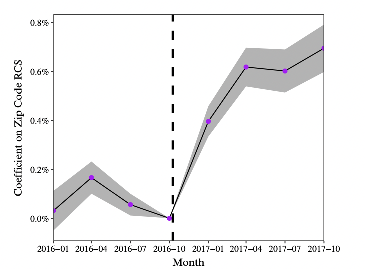
\includegraphics[width=\textwidth]{./figures/parker}}
    \begin{flushleft}
      {\footnotesize Note: Reproduced from \cite{meeuwis2018belief}, this figure reports regression coefficients of equity share on zip-code-level campaign contribution share to Republican candidates over an interval spanning the election.}
    \end{flushleft}
  \end{figure}
\end{verbatimwrite}%%%Slides
%%%Slides
  \begin{figure}[!ht] \centering  % [h!]
    \caption{ ~Portfolio responses to 2016 U.S. election}
    \label{fig:parker}
    \centerline{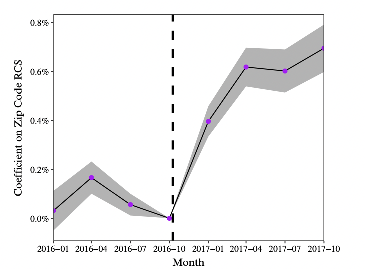
\includegraphics[width=\textwidth]{./figures/parker}}
    \begin{flushleft}
      {\footnotesize Note: reproduced from \cite{meeuwis2018belief}, this figure reports the baseline regression coefficients of equity share on zip-code level  campaign contribution share to Republican candidate for the three quarters prior to the election and the four quarters following the election, relative to allocations just before the election.}
    \end{flushleft}
  \end{figure}
%%%Slides

% Some remaining assumptions that could justify an `identical expectations' equilibrium would be (1) there is a single, unambiguous truth about the state of the world; (2) all agents who make an observation about the world would perceive the same truth; (3) all agents truthfully communicate all their observations to all their links instantaneously; (4) everyone agrees about the correct model of how the world works.'

% These assumptions effectively resurrect the identical expectations equilibrium in a framework where social communications exist, but achieve instantaneous and complete homogeneity in beliefs.  We can think of all of the epidemiological/network models discussed below as deviations, in one respect or another, from this perfect-trust instantaneous-transmission perfect-agreement framework.


\section{What insights can the epidemiological framework
  offer?}\label{what-insights-can-the-epidemiological-framework-offer}

\subsection{What Is an Epidemiological Framework?}
\label{subsec:epi_framework}

We will say that ideas, beliefs, `narratives,' or other mental states that affect behavior (henceforth, `expectations') result from an ``epidemiological'' process whenever they are modeled as resulting from some social interaction.

\ifthenelse{\boolean{inBook}}{T}{This is a slightly narrower scope than encompassed in textbook definitions of epidemiology, which include diseases that develop without any identifiable external influence.  The  epidemiological models we are interested in are those for ``transmissible'' diseases.

  But t}ransmission need not be person-to-person; it can reflect exposure to a ``common source.''  (Cosmic radiation to which everyone is exposed can cause diseases like cancer).  % People living in caves would be less susceptible; those on mountaintops, more.
In the context of beliefs, a natural interpretation of such a ``common source'' is news media (a point to which we return below).

\begin{comment}
  Having clarified this boundary, epidemiological models that are relevant for us vary in a few fundamental ways:
  \begin{quote}\normalfont
    \begin{enumerate}
    \item the states that agents could possibly experience
    \item the process by which an agent's state can change via social communication
    \item the channels of social communication
    \item heterogeneity or evolution over time that affects any of these
    \end{enumerate}
  \end{quote}
\end{comment}
In the simplest epidemiological model, a continuous population is partitioned among infected people {\Infected} and those who are susceptible {\Susceptible} but not yet infected, and the infectiousness of the `common source' is time-independent at probability $p$.  For a population at discrete date zero with a susceptible population of size 1, the dynamics of such a common-source SI model are given by Table~\ref{table:SIDyn}, with the obvious implication that as $n$ approaches infinity the entire population eventually becomes infected.

\begin{verbatimwrite}{./Tables/SIDynCS}
  \begin{table}[ht]
    \centering
    \caption{ ~Common Source \Susceptible\Infected~Model}\label{table:SIDyn} \medskip
    \begin{tabular}{ccc}
      \hline
      Date $t$ & Susceptible$_t$ & Infected$_t$ \\
      \hline
      0 & $1$  &  $0$ \\
      \hline
      1 & $(1-p)\phantom{^2}$ & $1-(1-p)\phantom{^2}$ \\
      \hline
      2 & $(1-p)^{2}$ & $1-(1-p)^{2}$ \\
      \hline
      $\vdots$ & $\vdots$ & $\vdots$ \\
      \hline
      $n$ & $(1-p)^{n}$ & $1-(1-p)^{n}$ \\
      \hline
    \end{tabular}
  \end{table}
\end{verbatimwrite}
  \begin{table}[ht]
    \centering
    \caption{ ~Common Source \Susceptible\Infected~Model}\label{table:SIDyn} \medskip
    \begin{tabular}{ccc}
      \hline
      Date $t$ & Susceptible$_t$ & Infected$_t$ \\
      \hline
      0 & $1$  &  $0$ \\
      \hline
      1 & $(1-p)\phantom{^2}$ & $1-(1-p)\phantom{^2}$ \\
      \hline
      2 & $(1-p)^{2}$ & $1-(1-p)^{2}$ \\
      \hline
      $\vdots$ & $\vdots$ & $\vdots$ \\
      \hline
      $n$ & $(1-p)^{n}$ & $1-(1-p)^{n}$ \\
      \hline
    \end{tabular}
  \end{table}

This framework can be extended in many directions.  The usual next step is for the disease to be transmitted as a result of `random mixing' where each susceptible person who encounters an infected person becomes infected with a fixed probability. Given a non-zero initial infected fraction $I_0$, the fraction  infected and susceptible evolve per Table \ref{table:SIDynTrans}.
\begin{verbatimwrite}{./Tables/SIDynTrans}
  \begin{table}[ht]
    \caption{ ~Transmissible SI Model}\label{table:SIDynTrans}
    \centering\medskip
    \begin{tabular}{ccc}
      \hline
      Date $t$ & Susceptible$_{t}$ & Infected$_{t}$ \\
      \hline
      0 & $S_0$  &  $I_0$ \\
      \hline
      1 & $S_0 - \beta S_0I_0$ & $I_0+\beta S_0I_0$ \\
      \hline
      2 & $S_1-\beta S_1I_1$ & $I_1+\beta S_1I_1$ \\
      \hline
      $\vdots$ & $\vdots$ & $\vdots$ \\
      \hline
      $n$ & $S_{n-1}-\beta S_{n-1}I_{n-1}$ & $I_{n-1}+\beta S_{n-1}I_{n-1}$ \\
      \hline
    \end{tabular}
  \end{table}
\end{verbatimwrite}
  \begin{table}[ht]
    \medskip
    \caption{ ~Transmissible SI Model}\label{table:SIDynTrans}
    \centering\medskip
    \begin{tabular}{ccc}
      \hline
      Date $t$ & Susceptible$_{t}$ & Infected$_{t}$ \\
      \hline
      0 & $S_0$  &  $I_0$ \\
      \hline
      1 & $S_0 - \beta S_0I_0$ & $I_0+\beta S_0I_0$ \\
      \hline
      2 & $S_1-\beta S_1I_1$ & $I_1+\beta S_1I_1$ \\
      \hline
      $\vdots$ & $\vdots$ & $\vdots$ \\
      \hline
      $n$ & $S_{n-1}-\beta S_{n-1}I_{n-1}$ & $I_{n-1}+\beta S_{n-1}I_{n-1}$ \\
      \hline
    \end{tabular}
  \end{table}


The best-known epidemiological framework adds an `\Recovered' state that can designate either recovery or `removal' (via, say, death), yielding the `classical' SIR models.\ifthenelse{\boolean{inBook}}{}{\footnote{Unfortunately, the model's equations do not have finite closed-form analytical solutions; \cite{miller2012note} and \cite{harko2014exact} produce alternative formulations of what they call analytical solutions -- see   \href{https://en.wikipedia.org/wiki/Compartmental_models_in_epidemiology\#Transition_rates}{this Wikipedia page} -- but both involve an integral that can only be calculated numerically.}}
The SIR framework has rich and interesting implications, such as the potential for `herd immunity' which comes about when a high enough proportion of the population has either Recovered or otherwise been Removed (say, by vaccination) from the Susceptible compartment.

% so implications must be obtained numerically.  %using numerical computational procedures -- though with current computational technologies such computations for the original \cite{kermack_contribution_1927} model have negligible cost.

Options proliferate from there.\footnote{For a general introduction to these model basics, we refer the reader to \href{https://en.wikipedia.org/wiki/Compartmental_models_in_epidemiology\#Transition_rates}{this Wikipedia page}.  Prominent examples include	 \href{https://www.ncbi.nlm.nih.gov/pmc/articles/PMC3710332/}{\cite{bailey1975mathematical}}, \href{https://www.amazon.com/Infectious-Diseases-Humans-Dynamics-Control/dp/019854040X}{\cite{anderson_infectious_1992}}, \href{https://epubs.siam.org/doi/abs/10.1137/S0036144500371907}{\cite{hethcote_mathematics_2000}}, \href{https://www.ncbi.nlm.nih.gov/pmc/articles/PMC6001967/}{\cite{brauer2017mathematical}}.}  A framework in which there are two possible outcomes of the infection, recovery or death, receives the acronym SIRD.  If the disease is one in which it is necessary to track the proportion who have been Exposed but are not yet (and may never become) infected, the result is an SEIR model -- and so on.

% Some variants do not have additional states but allow additional transitions among the states already treated (presumably, except for state `D'). For instance, the SIS model allows the infected (I) to transit back to susceptible (S) if immunity to the disease declines after some time.

\ifthenelse{\boolean{inBook}}{}{
  One standard assumption for all of these models is that agents are \textit{ex-ante} homogeneous, but the classical framework can be extended to permit various kinds of heterogeneity -- at the considerable cost of adding whole new systems of nonlinear differential equations.  An advantage of the network approach is that since it is solved by simulation, modifications of the model are much easier to make because they do not add new systems of simultaneous differential equations to be solved.
}

% Another extension of these models incorporates the possibility that some agents may take protective actions to change the transition probabilities, instead of taking them all as exogenous.

% We will stop our description of the  epidemiological literature here because our purpose was more to introduce the kinds of modeling assumptions that are often considered there.

% Some of the disease states above have a natural interpretation in a model of expectations: A person who has adopted an idea from someone else can be said to have been `infected' by that idea.  Some are less natural; e.g., there is usually not an obvious analog in expectations models of the `recovered' state. % (though our survey below will describe some examples).

% The art of building a good model boils down to the choices articulated above: states, transitions, and the nature of heterogeneity.

% In some dimensions, close analogies can be drawn between the two applications.  Like an infected disease, an idea/opinion/certain view of the economy can spread via interpersonal contacts from those who have held it already, i.e. the infected (I) to those who are exposed to it (E) or who are potentially receptive to them (S), and it may also be forgotten, i.e. recovery (R).  Furthermore, the agents could be either ex-ante homogeneous or heterogeneous and the transmission of the expectations could be specific to agent types and their locations in the network.

\subsubsection{Adapting the Disease Metaphor to Expectations}\label{subsubsec:AdaptingTheModel}
\hypertarget{AdaptingTheModel}{}

Basic epidemiological models usually study the dynamics of a single disease in a population, with a natural terminal stage like recovery or death.  Economists will often be interested in keeping track of how expectations change about an aggregate variable like stock prices, which does not have a terminal point and in which many competing opinions may infect different people at the same time.

An advantage of network-theory tools is that they can easily accommodate ways in which an economic application may call for such modifications.  It is trivial  to represent as many competing `diseases' (e.g., theories of stock prices) as desired, and there is no need to specify a `recovery' state.

To take a more complex example, in classical epidemiological models it would be painful to capture dynamics of a disease in which people become  `more infected' after repeated contact with other infected people.  But in a network model, it is easy to capture the proposition that a person may need to be exposed to an idea more than a certain number of times, or from more than a given number of sources, before they will adopt it -- as proposed in \cite{granovetter1978threshold}, and as implemented in \cite{jackson2007diffusion}.\footnote{See the interesting discussion of such `threshold models' in \cite{glasserman2016contagion}.}

% Another direction that epidemiological expectations models constructed by economists might take is to consider the implications of purposive behavior that might enhance (or impede) the flow of information.  For example, the widely used Michigan Survey of Consumers asks respondents their views on long term interest rates. If the respondent is one who recently bought a house, they may have deliberately `infected' themselves by doing some research on mortgage interest rates; in that case they might resemble a fully informed  agent.  But after the homebuyer has obtained a mortgage, there may be little  reason  for them to pay attention to long run interest rates.  It is not implausible that their views on rates will be shaped passively by random encounters with news sources or friends -- encounters that are better understood with an epidemiological framework than in a model in which the consumer is either perpetually fully informed or, for that matter, perpetually calculating the exact degree to which it would be optimal for them to choose to be fully informed.

% But there should be limits.  For EE as a framework to be sufficiently well-defined to be useful as an alternative to RE or other general-purpose expectational frameworks, it seems likely that it will be necessary to rule out the complexities that can arise in game theoretic uses of network theory.    The natural way to do that is to assume that consumers believe themselves to be infinitesimal:  They believe that they do not, personally, have the ability to affect equilibrium outcomes that matter to them.

% Using the foregoing introduction as a high-level map and definition of terms, our next section explores in some detail the varieties of ``epidemiological'' modeling strategies that have been used (or could be used) for economic modeling.

\begin{comment}% Not sure what good this "plausible applications" section does here -- maybe move to conclusion?
  \subsection{Plausible Applications of Existing  Tools to Economics}

  We begin by sketching, among the many directions the epidemiological literatures have already explored, the ones likely to be most useful to economists.

  \begin{itemize}
  \item  How geography structures the connections between people
  \item The structures of social networks as measured by social media connections
  \item  Consequences of heterogeneity in, say, likelihood of infection given exposure
  \item  Characteristics of models in which people's views do not converge but instead may result in groups of like-minded people \citep{meeuwis2018belief}.
  \end{itemize}

  The explicit end goal of much recent work has been to construct models that can match some of the newly available forms of data that we can increasingly map in high fidelity.

  % Math
  % While the original model of \cite{kermack_contribution_1927} and its immediate descendants were represented by simple differential equations that could be analyzed by hand, today's epidemiological models have become so complex that they cannot be studied effectively with pen and paper.  Instead, the details of the framework are constructed, then a population of simulated agents is created who abide by those rules of the game, and the population is simulated computationally in order to determine the model's implications.  (Reference the notebook again).  A paper is viewed as a finished contribution if it matches some of the patterns in a dataset.

  A highly cited example \cite{bauckhage2011insights} which uses a variety of epidemiological models in an attempt to explain the dynamics of
  popular internet ``memes.'' The attempt meets with some success in the sense that the author finds some examples in which one of the many
  variants of the SIR, SIER, and epidemiological frameworks seem to (ex post) be able to match the spread of, say, a photograph of a laughing baby, or the ``montauk monster.''  Much of the analysis has been somewhat solipsistic, in the sense that there is often not any attempt to measure (much less to model) knock-on consequences for variables other than the information itself.

  A more recent literature has examined the differential rates at which different kinds of ``news'' spreads, reaching an interesting conclusion that ``misinformation'' seems to spread more readily than true stories\citep{vosoughi_spread_2018}. And there is a rapidly growing literature on potential implications of the spread of ideas for political outcomes like election victories \citep{allcott2017social, grinberg2019fake} -- though even papers in that literature often do not present an integrated analysis of the structural mechanisms of the epidemiological process with the empirical consequences at the ballot box.

  And we are not aware of any papers in this vast literature in which there is a mapping from the structure of a model to an economic outcome that is a consequence of that structure, much less of a fully rounded model that explores the ramifications of that economic outcome on future dynamics of ideas.

  The best way to view all of this is probably as an arbitrage opportunity: Economists can take models of belief dynamics created in this literature and plug them into an economic model to determine their consequences (if any) for an economic phenomenon of interest, with standard economic modeling supplying the elements of the criteria above (like feedback between the spread of ideas and the economic outcomes) that are missing from the existing literature.
\end{comment}


\subsection{One Example}\label{subsec:SIRModel}
\label{subsec:shillerpound}
Here, we provide a specific example of an economic question formulated in a thoroughgoing epidemiological way.  Our present purpose is not to extract economic insights -- we do that in section~{\ref{subsec:assetprice}} below -- but simply to illustrate how the epidemiological toolkit works.

\IfPrivate{\href{https://github.com/iworld1991/EpiExp/blob/master/Literature/shiller1989survey.pdf}{\cite{shiller1989survey}}}{\cite{shiller1989survey}} use an SIR model to capture how interest in particular stocks spreads;\ifInBook{\footnote{This paper builds on the earlier work comparing the efficient market hypothesis of stock prices and an alternative model incorporating social dynamics \IfPrivate{\href{https://github.com/iworld1991/EpiExp/blob/master/Literature/shiller1984stock.pdf}{\cite{shiller1984stock}}}{\cite{shiller1984stock}}. }}
{\footnote{Our treatment makes two inconsequential modifications.  First, in order to be able to instantiate the model using the \href{https://ndlib.readthedocs.io/en/latest/}{\texttt{NDLib}} computational toolkit described below, we rewrite the originally continuous-time model in a discrete-time form. Second, the original paper described an additional stochastic shock to the change in $I_t$ meant to capture a potential ``change in the `source' of the infection or the nature of the contagion.''  Because that shock was not actually used for any results in the paper, we neglect it in our exposition.}}% CDC to TW: Make sure this is explained in the notebook. % We have had them in the notebook now.
 we examine a model almost identical to theirs.
At date  $t$, a large population of investors measured by the real number $N$ is divided into three ``compartments.''  (See Figure \ref{fig:sir_diagram}).  $I_t$ investors are currently ``infected'' with interest in a certain stock;  $S_t$ investors are not infected but are ``susceptible'' to becoming interested; and $R_t$ measures investors who have been ``infected'' but have ``recovered'' from the infection.\footnote{For our purposes here, we do not need to define the exact consequences of `recovery.'  See below (or see the original paper) for further discussion.}


\begin{verbatimwrite}{./Slides/FigureSIRFlowDiagram}%%%Slides
	\begin{figure}[!ht] \centering  % [h!]
		\caption{ ~A SIR model of stock investors}
		\label{fig:sir_diagram}
		\centerline{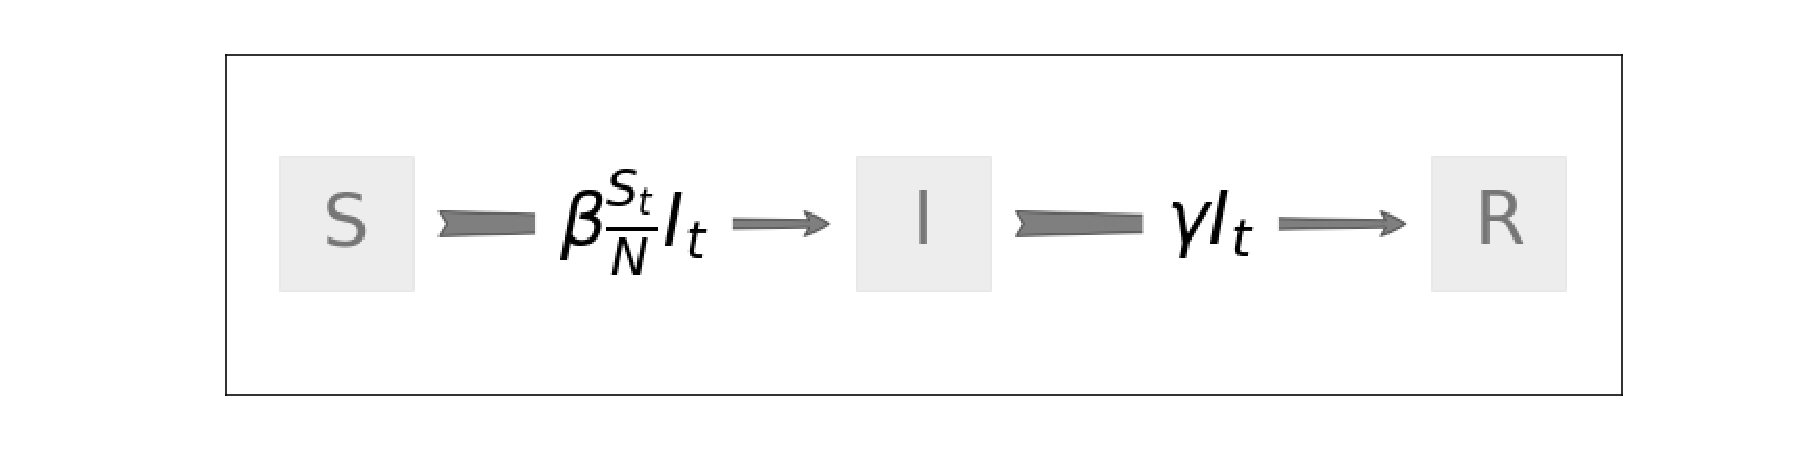
\includegraphics[width=\textwidth]{./figures/flow_diagram}}
		\begin{flushleft}
			{\footnotesize Note: This graph plots the transitions between different compartments in the SIR model of stock investors described in \cite{shiller1989survey}. }
		\end{flushleft}
	\end{figure}
\end{verbatimwrite}%%%Slides
%%%Slides
	\begin{figure}[!ht] \centering  % [h!]
		\caption{ ~A SIR model of stock investors}
		\label{fig:sir_diagram}
		\centerline{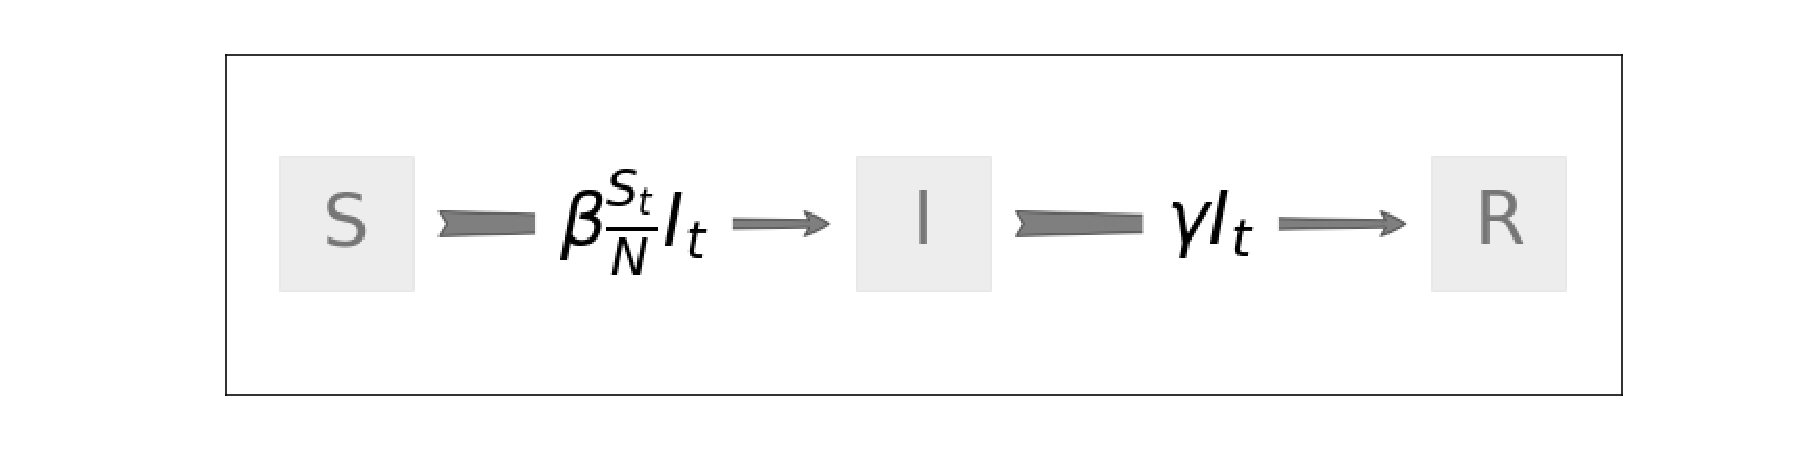
\includegraphics[width=1.5\textwidth]{./figures/flow_diagram}}
		\begin{flushleft}
			{\footnotesize Note: This graph plots the transitions between different compartments in the SIR model of stock investors described in \cite{shiller1989survey}. }
		\end{flushleft}
	\end{figure}


Under `random mixing,' each person is expected to have contact with $\contactNum$ others, randomly selected from the entire population.  The only kind of contact with any consequence is between an infected and a susceptible person: Such an encounter has a probability $\tranProb$ of causing the susceptible person to become infected.

Epidemiological models typically define a parameter $\beta$ that combines consequences of the rate of social contact $\contactNum$ and the rate of transmission upon  contact, $\tranProb$:\ifInBook{}{\footnote{In any SIR model embedding an explicitly defined connection network by which the ``disease'' spreads, $\beta$ is the product of the average number of connected nodes (``degree''), and the infection probability conditional on contact. For instance, in a random graph (\cite{erdos1960evolution})  with connection probability $p$ and the size of network N, the average contacts every agent has is $(N-1)p$. }}
\begin{verbatimwrite}{./Equations/beta}
\begin{equation}
	\label{eq:beta}
    \beta  = \tranProb \contactNum.
\end{equation}
\end{verbatimwrite}
\begin{equation}
	\label{eq:beta}
    \beta  = \tranProb \contactNum.
\end{equation}


The expected number of new infections generated in period $t$ (corresponding to the decline in the number of susceptible persons) can now be calculated: Fraction $S_{t}/N$ of an infected person's contacts will be susceptible, so the number of newly generated infections per infected person will be $\tranProb \times \contactNum \times (S_{t}/N).$ The `infected' population also changes because every infected person recovers with a probability of $\gamma$ per period.

Putting these elements together, the  changes in the population in different compartments are given by
\begin{equation}
	\label{eq:sirdyn}
	\begin{split}
	&	\Delta S_{t+1} = -\beta I_{t}(S_{t}/N) \\
	&	\Delta I_{t+1} = \beta \frac{S_{t}}{N}I_{t} - \gamma I_t \\
&		\Delta \Recovered_{t+1} = \gamma I_t.
	\end{split}
\end{equation}

%The term $\beta \frac{S_{t}}{N}I_{t}$ captures the number of people who ``flow'' from ``compartment $S$'' to ``compartment $I$'', which is proportional to the infection rate $\beta$, the fraction of people who are susceptible $\frac{S_t}{N}$, and the number of the infected $I_t$. The  term $\gamma I_t$ captures the number of people who ``flow'' from $I$ to $\Recovered$


\begin{verbatimwrite}{./Slides/FigureSIRSimulation}%%%Slides
    \begin{figure} \centering  % [h!]  [!ht]
        \caption{ ~Simulated dynamics from a SIR model of stock investors}
        \label{fig:sir_simulate}
        \centerline{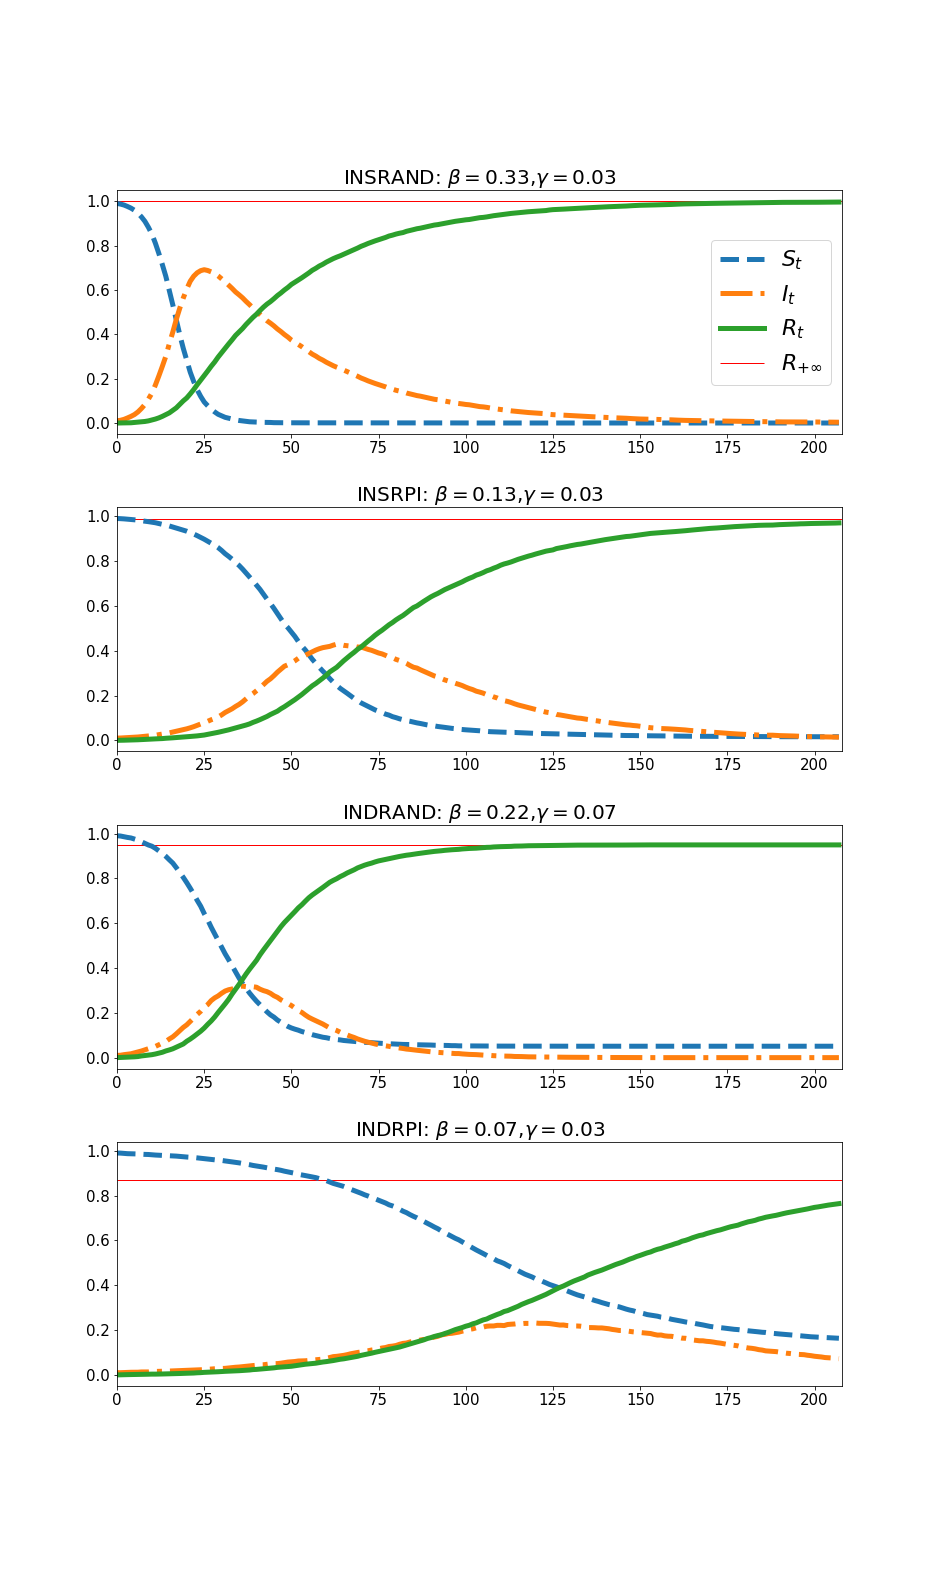
\includegraphics[width=0.85\textwidth,height=0.85\textheight]{./figures/sir_simulate}}
        \begin{flushleft}
            {\footnotesize The four figures respectively simulate an SIR model under calibrations corresponding to \cite{shiller1989survey}'s parameter estimates for (1) institutional investors for a randomly selected stock (INSRAND); (2) institutional investors for a rapidly rising stock (INSRPI); (3) individual investors for a random stock (INDRAND); and (4) individual investors for a rapidly rising stock (INDRPI). The susceptible population {\Susceptible} is dashed; dash-dot shows the size of the {\Infected} compartment, and the recovered population {\Recovered} is solid.  The horizontal thin solid line corresponds to the limiting size of compartment of $R$ in the long run.  To reproduce these figures, see the companion \href{https://github.com/llorracc/EpiExp/blob/master/SIR_Ndlib.ipynb}{Jupyter Notebook}. }
        \end{flushleft}
    \end{figure}
\end{verbatimwrite}%%%Slides
%%%Slides
  \begin{figure} \centering  % [h!]  [!ht]
    \caption{ ~Simulated dynamics from an SIR model of stock investors}
    \label{fig:sir_simulate}
    \centerline{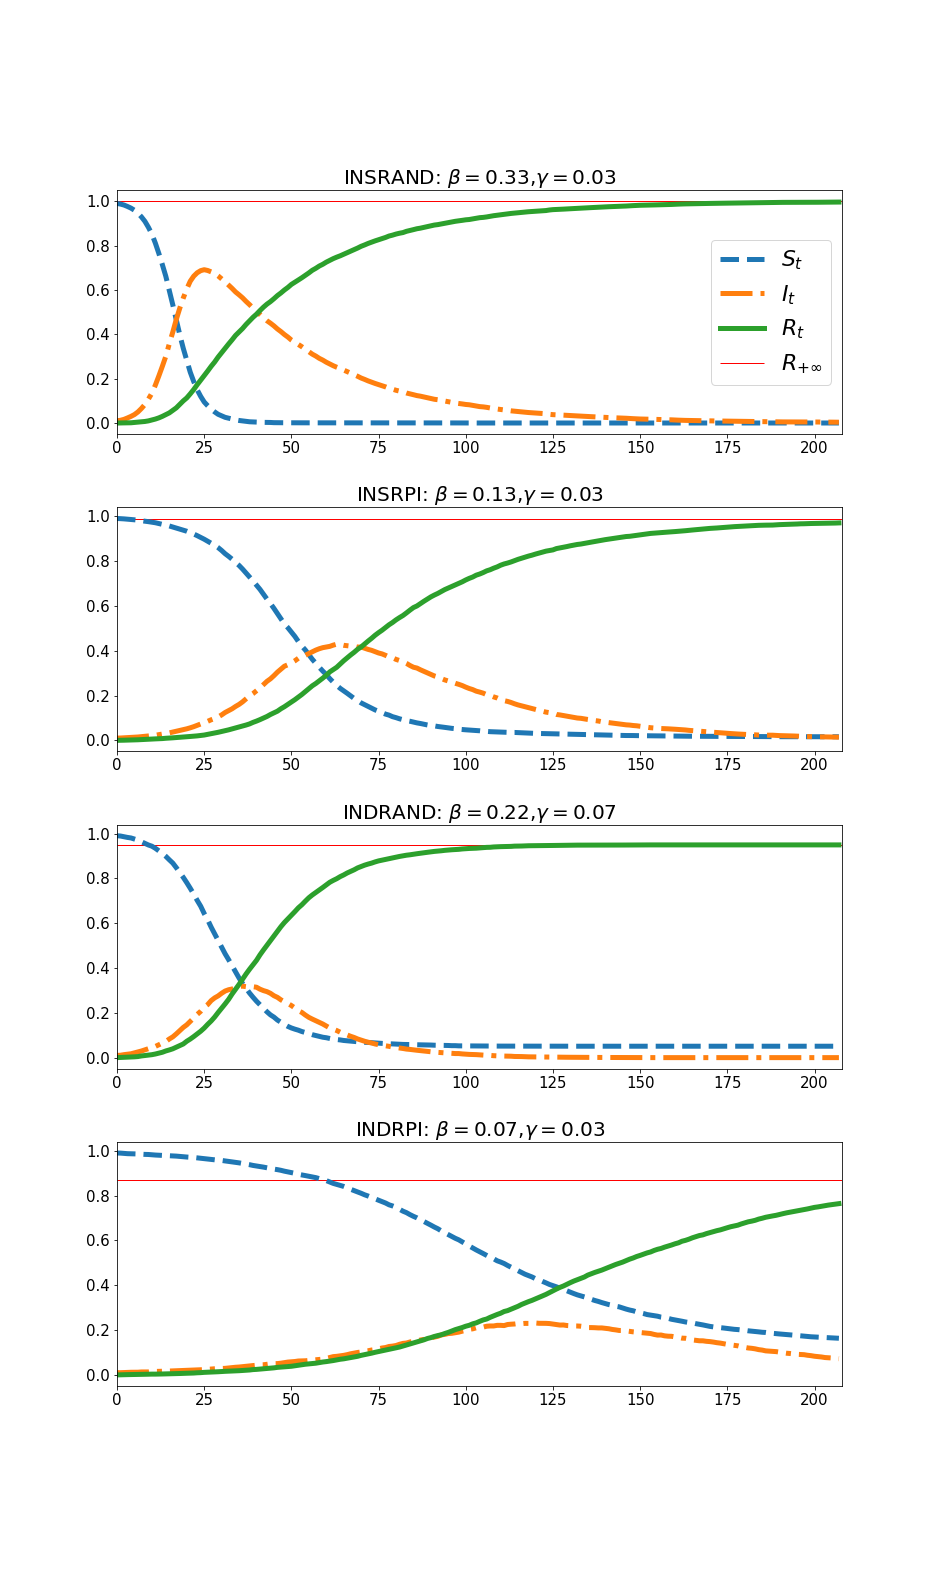
\includegraphics[width=0.85\textwidth,height=0.85\textheight]{./figures/sir_simulate}}
    \begin{flushleft}
      {\footnotesize Note: This graph plots the simulated paths of populations in different compartments in a SIR model of stock investors, as described in \cite{shiller1989survey}. We use the median estimates of the infection rate $\beta$ and recovery rate $\gamma$ for four samples: institutional investors for a randomly selected stock (INSRAND), institutional investors for a rapidly rising stock (INSRPI), individual investors for a random stock (INDRAND), and individual investors for a rapidly rising stock (INDRPI). The horizontal thin solid line corresponds to the limiting size of compartment of $R$ in the long run. The simulation is done with the Python library \href{https://ndlib.readthedocs.io/en/latest/}{``NDlib''}, for details, see the companion \href{https://github.com/llorracc/EpiExp/blob/master/SIR_Ndlib.ipynb}{Jupyter Notebook}. }
    \end{flushleft}
  \end{figure}
%%%Slides

The simplest special case of the SIR model is one with a recovery rate of $\gamma=0$, in which case the model reduces to the transmissible SI model discussed in Section \ref{subsec:epi_framework}.  Another straightforward case is $\beta < \gamma$, in which from any starting point the population of infected persons $I$ gradually dies down to zero.

\newcommand{\Rzero}{\mathcal{R}(0)}
The interesting cases emerge when the `basic reproduction ratio' $\Rzero = (\beta/\gamma)$ exceeds one (this $\Rzero$ is unrelated to the $\Recovered$ used elsewhere to measure the recovered population), because $\Rzero > 1$ guarantees that an initial arbitrarily small infection will grow, at least for a while (assuming that at the beginning everyone is susceptible, $S_{0}/N = 1$).

To illustrate the model's implications, we configure it with four combinations of parameter values taken from \cite{shiller1989survey}, characterizing two different kinds of investors and two categories of stocks.  %(Section~\ref{subsec:assetprice} describes the investors and stock categories, and interprets the economics; here we confine our observations to the epidemiology.)


We calculate the quantitative implications using one of the best of the many computational toolkits for analyzing such models that have proliferated in recent years:  %\footnote{For the simulation of the SIR model we use the Python library \href{https://ndlib.readthedocs.io/en/latest/}{NDlib} (\cite{rossetti2018ndlib}), which builds upon another Python library called NetworkX (\cite{hagberg2008exploring}).}
\href{https://ndlib.readthedocs.io/en/latest/}{NDlib} lets users specify an arbitrary network structure on which a disease might spread. We exploit the above-mentioned fact that a random-mixing SIR model can be approximated with an \textit{ex-ante} generated random graph when the transmission probability $\tau$ and the average number of connections $\chi$ in the graph are configured such that their product is equal to the calibrated infection rate $\beta$ (see Equation \ref{eq:beta}).\footnote{See the companion \href{https://github.com/llorracc/EpiExp/blob/master/SIR_Ndlib.ipynb}{Jupyter Notebook} of this paper for our  implementation.}

In Figure \ref{fig:sir_simulate} the vertical axis measures the populations of {\Susceptible}, {\Infected}, and {\Recovered} investors; time since the initial date of infection is on the horizontal axis.  Also plotted is the limiting size of the recovered compartment\ifInBook{.}{, for which an analytical solution exists.\footnote{Given a constant basic reproduction ratio $\beta/\gamma$ that is strictly greater than $1$, and an initial fraction $S_{0}/N$ close to 1, the limiting fraction of $\Recovered$, denoted as $\recovered_{+\infty} = \Recovered_{+\infty}/N$, is the solution to the implicit equation: $e^{-\frac{\beta}{\gamma} r_{+\infty}} = 1-r_{+\infty}$.  See  \href{https://en.wikipedia.org/wiki/Compartmental_models_in_epidemiology\#Transition_rates}{this Wikipedia page}, \cite{harko2014exact}, \href{{https://iopscience.iop.org/article/10.1088/1751-8121/abc65d}}{\cite{kroger2020analytical}}, and \cite{okabe2021microscopic} for details of the results.}} % CDC to TW: Move the contents of this footnote to the Jupyter notebook (adding the papers to the nocite list)

Two common patterns emerge.  First, since in all four cases the basic reproduction ratio $\Rzero$ is greater than 1, in all four cases there is an outbreak. The size of the infected population first expands to its maximum value and then gradually levels off to zero, exhibiting a hump-shaped ``viral curve'' characteristic of SIR models.  Second, in all scenarios, the system ultimately converges to a steady-state where most people have cycled through infection and recovery. Even in the case with the smallest reproduction ratio, the proportion who cycle through the process of Infection and Recovery is almost 85 percent, implying a high degree of infectiousness. Under other configurations, the limiting size of the infected-then-recovered `compartment' $R$ is close to 100 percent.

The main difference in the parameterizations is the speed with which these eventualities play themselves out, which varies considerably.  (For a discussion of the model's economic (as distinct from epidemiological) content see Section~\ref{subsec:assetprice}).

%Even using the results of their own surveys explicitly designed for the purpose, \cite{shiller1989survey} needed to exercise considerable ingenuity to produce the calibrations we have used above.

%We highlight~\cite{shiller1989survey} here because it presents an early but rich example that satisfies all our criteria for an epidemiological model of economic expectations. First, it articulates and a explicit structural mathematical mechanism by which an idea (in this case, interest in a stock) spreads in the population as a result of social communication. Second, the model has clear assumptions and predictions for both the micro and macro dynamics of expectations, which can be tested (or calibrated) with measurable survey data (indeed, they were calibrated with data that~\cite{shiller1989survey} collected themselves because existing sources had not asked the right questions).  Third (as we explain in section~{\ref{subsec:assetprice}}), dynamics of separately measurable economic phenomena (stock prices) are hypothesized to be a consequence of the dynamics of those expectations.  % Not many papers satisfy all these criteria.



\hypertarget{literature}{}
\section{Literature}\label{sec:literature}

% \subsection{Three Fields With Full-Fledged EE Models}

% \centerline{ [Insert Figure \ref{fig:graph_mixer} here]}


\begin{figure}[!ht] \centering  % [h!]
  \caption{ ~Literature map of cited papers}
  \label{fig:graph_mixer}
  \centerline{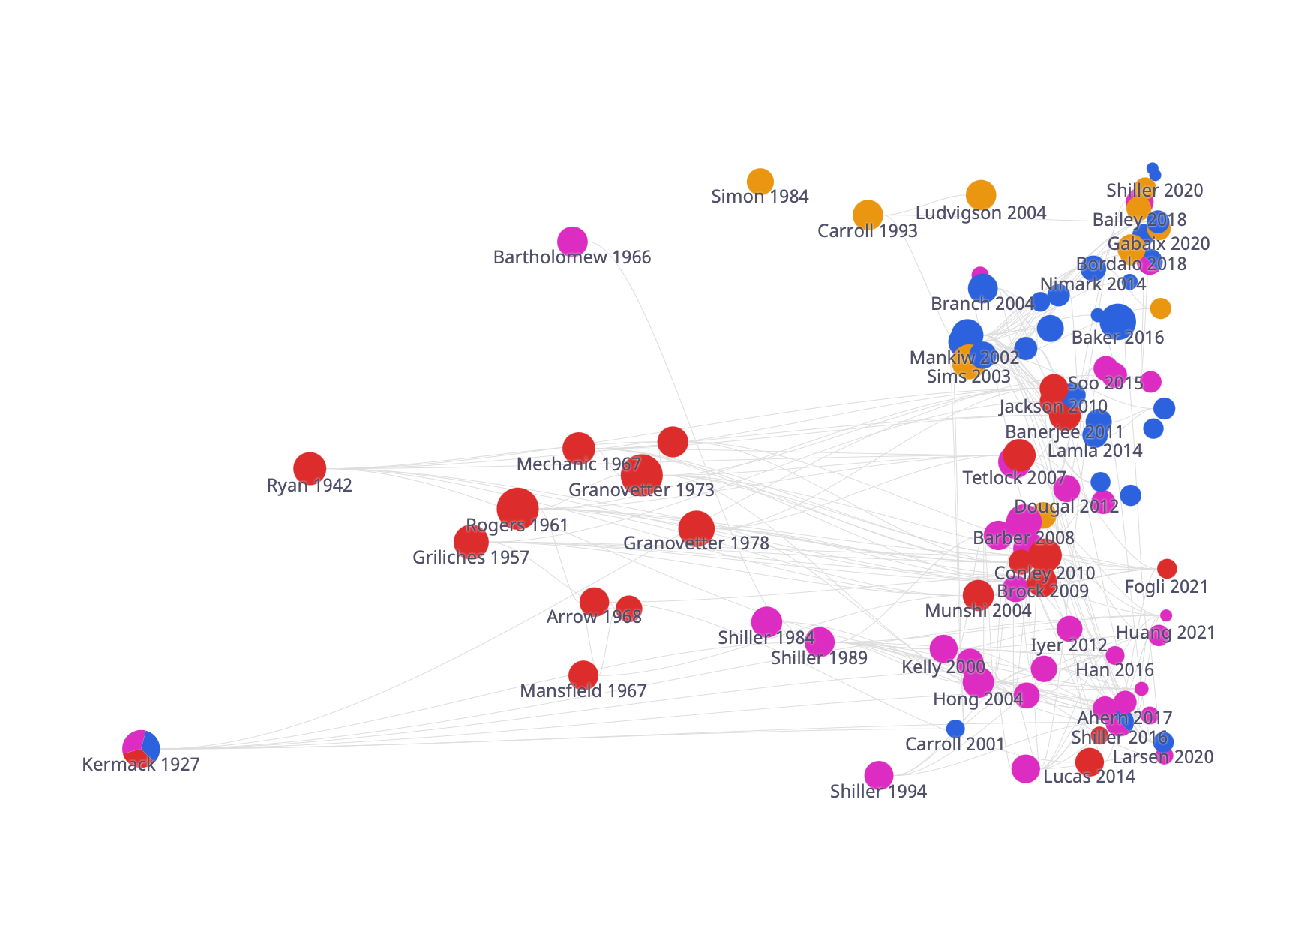
\includegraphics[width=\textwidth]{./figures/graph_mixer}}
  \begin{flushleft}
    {\footnotesize Note: Papers we have identified as having a strong epidemiological flavor in three literatures in economics: technological diffusion (red), asset markets (purple), and macroeconomic expectations (blue).  Papers in yellow have no epidemiological content but are cited in the text as having content that may be interesting to EE modelers. See \href{https://app.litmaps.co/shared/89EF6E28-98E7-4406-AA0F-BE8045A0571C}{here} for an interactive version.}  % CDC to TW: It would be nice if when someone clicks the link they got to see all the submaps as well as the joint one.  Also, the version I get when I click the link does not have the different literatures in different colors ...  TW:   there is no way to have those colors. Colors are only avaiable for a particular workspace with exactly the four submaps together and they will be colored according to those submaps. But a generally shared one does not know which paper is from which.  Also, since only map can be shared, not workspace, so it is hard to have all maps in one link.
  \end{flushleft}
\end{figure}

Figure~\ref{fig:graph_mixer} provides a citation map of papers in the literatures we discuss here; the thin lines represent a citation from the later paper to the linked earlier one.


\subsection{Diffusion of Technology}\label{subsec:techDiffusion}

%\begin{center}	[Insert Figure \ref{fig:graph_diffusion}  here]\end{center}

\begin{figure}[!ht] \centering  % [h!]
	\caption{ ~Literature map of EE models of technological diffusion}
	\label{fig:graph_diffusion}
	\centerline{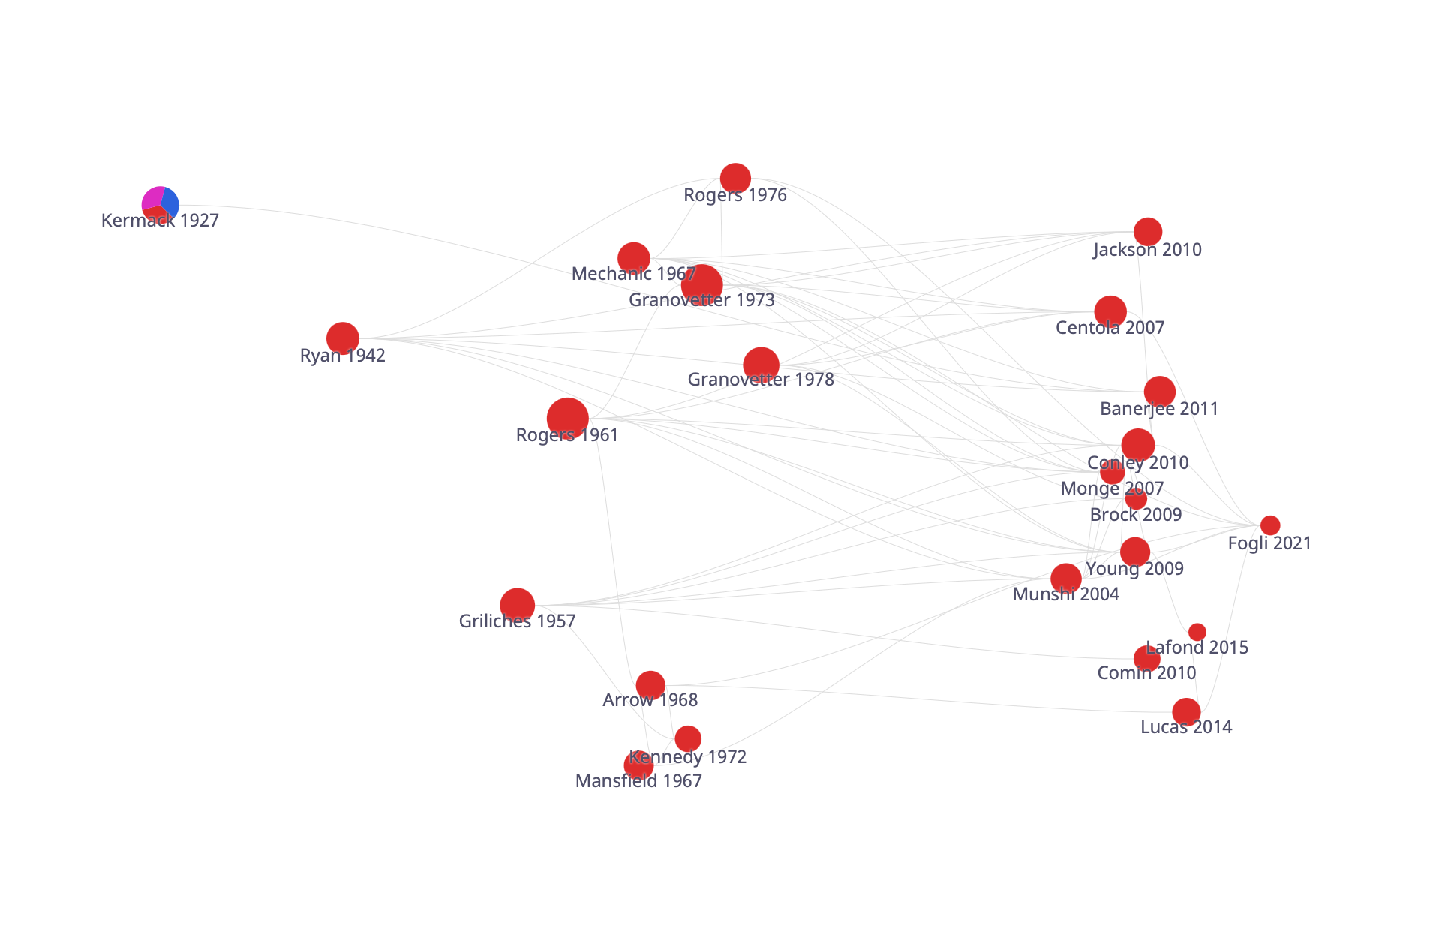
\includegraphics[width=1.5\textwidth]{./figures/graph_diffusion}}
	\begin{flushleft}
		{\footnotesize Note: This graph includes selected papers under the topic of epidemiological modeling of technological/innovation diffusion in economics and closely related literature from other fields. See \href{https://app.litmaps.co/shared/1D9003CB-75FE-4633-B60A-79B70E03B691}{here} for an interactive version.}
	\end{flushleft}
\end{figure}

%Economists have understood since \cite{solow1956contribution} that technological progress is the wellspring of economic growth.  Although in studies of the process by which fundamentally new technical knowledge is generated, we are not aware work that could be classified as epidemiological, the vast bulk of technological progress for most of the individual agents who are progressing does not reflect their independent invention of ideas novel to humanity -- it reflects their adoption of knowledge invented by others.  In recognition of this fact, an extensive literature has studied a topic usually identified as `the diffusion of technology.'  Traditionally, this line of work has been seen as separate from the domain of economic expectations.  But the reason for adopting a new technology is surely that there is an expected gain from doing so, a point that is explicitly made at various places in the more theoretically-minded branches of the literature.

\href{https://github.com/iworld1991/EpiExp/blob/master/Literature/arrow_classificatory_1969.pdf}{\cite{arrow_classificatory_1969}} draws an explicit analogy between the diffusion of ideas and the spread of disease.  (His paper is one of the earlier contributions from the economics literature captured in Figure~\ref{fig:graph_diffusion}; see Section~\ref{subsec:nonecon} for work outside of economics on the diffusion of scientific knowledge.)

Arrow puts interpersonal communication at the center of knowledge diffusion and the consequent economic growth, and argues that the speed of knowledge diffusion may account for international differences in both levels and dynamics of income per capita. He conjectures that the speed of knowledge diffusion is influenced by factors that he explicitly compares to  those that influence the spread of disease including (1) the perceived reliability of the sender (which affects infectiousness); (2) socioeconomic traits (which affect exposure and susceptibility); (3) the understandability of information by the receiver (degree of immunity); and so on.

Arrow's interpretation is the step that puts technological diffusion squarely in the realm of EE modeling, under the mild further assumption articulated above: That what spreads is the `expectation' that adoption of the technology will yield higher productivity (expectations were not explicitly modeled because Arrow's seminal research predated the era when expectations were solicited on surveys; but expectational questions of exactly this kind have been asked in more recent work on diffusion, see~\cite{banerjee2013diffusion}, and unsurprisingly confirm that people adopt a technology when they expect it to be beneficial).

Closely related to Arrow's work on technological progress is work by \href{https://en.wikipedia.org/wiki/Diffusion_of_innovations}{\cite{rogers1962diffusion}}, who popularized a theory of the ``diffusion of innovations'' based on a meta-analysis of early studies of the spread of ideas within many academic disciplines.\footnote{Though Rogers was a sociologist, we include his work in the discussion here because it has had such a strong impact on the subsequent economics literature.}  The factors that this literature identifies as determinants of the dynamics of diffusion are directly interpretable as corresponding to the ``infectiousness'' of the idea, the degree to which populations are ``exposed'' to the idea, and many of the other elements of the epidemiological frameworks sketched below.

\href{https://github.com/iworld1991/EpiExp/blob/master/Literature/young2009innovation.pdf}{\cite{young2009innovation}} is a broader survey of how alternative epidemiological models of technological diffusion generate different shapes of  ``adoption curves'' with consequent effects on the path of economic growth. He shows that how the shape of diffusion curves differs in models of `inertia' (a SI common-source model), `social influence' (a threshold model), `contagion' (a standard transmissible SI model), and `social learning,' where learning is based on observed actions of others.\footnote{We do not survey a large parallel literature on technology/innovation diffusion in economics that features the role of social learning, as this work is not explicitly built upon epidemiological frameworks. Examples  include  \href{https://www.researchgate.net/publication/222676428_Social_Learning_in_a_Heterogeneous_Population_Technology_Diffusion_in_the_Indian_Green_Revolution}{\cite{munshi2004social}},   \href{https://www.jstor.org/stable/41038754}{\cite{comin2010exploration}} and so on.}  % the first one is field evidence on tech diffusion in Indian showing that information flow is weaker when  underlying hterogeneity is higher.  The scond  builds the process of tech diffusion  into a neocalssical growth model.


\href{https://pubmed.ncbi.nlm.nih.gov/23888042/}{\cite{banerjee2013diffusion}} estimates an epidemiological model based on the real-world network and pattern of the diffusion of microfinance in a number of Indian villages. The paper provides direct evidence for word-of-mouth diffusion of beliefs through a social network. The model differentiates between agents who simply adopt the technology because they have heard about it from others (an `information passing mechanism') and those who have adopted due to others' participation (an `endorsement mechanism'). This is an example of how standard epidemiological models can be extended to incorporate alternative infection rules to accommodate more sophisticated applications.

\cite{lucas2014knowledge} construct a model economy containing agents with a distribution of levels of productivity, and consider the dynamics of aggregate productivity under several alternative assumptions about the ways in which agents with lower productivity can `learn' from agents with higher productivity.  (`Learning' in their model just means that, in an encounter between two agents, the agent with lower productivity adopts the other agent's technology).  %Encounters between agents are of the standard epidemiological `random mixing' kind.
% The baseline version of the model is one in which every agent is eligible to adopt any technology they encounter, which corresponds roughly to an epidemiological assumption that the `disease' is equally transmissible to all agents.  They also consider an alternative in which it is easier to move to a technology that is `near' your own than to leap across a large technological gap.  This latter assumption can perhaps be thought of as being similar to the `threshold' mechanisms discussed above, in which an idea is more likely to be transmitted if an agent is exposed to it many times -- assuming that agents are more likely to encounter other agents whose productivity levels are similar to their own.

A particularly interesting feature of this model is that the agents solve an optimization problem to determine the intensity of their search effort, which affects the likelihood of encountering ``better technology.''  %; this framework is constructed so that the agents have enough knowledge of the productivity distribution (and the efficacy of search) to make such choices rationally.
This is likely to be a common direction in which economists may take epidemiological models: Incorporation of purposive behaviors by agents. While some work in epidemiology also allows agents to take actions to reduce the probability of infection, models in that literature have rarely been formulated with an eye to creating a structure where an explicit analytical optimization problem can be stated and solved.

% CDC: this is where Lucas and Moll's paper should be surveyed.
% Abstract:  We analyze a model economy with many agents, each with a differ- ent productivity level. Agents divide their time between two activi- ties: producing goods with the production-related knowledge they already have and interacting with others in search of new, productivity- increasing ideas. These choices jointly determine the economy’s cur- rent production level and its rate of learning and real growth. We construct the balanced growth path for this economy. We also study the allocation chosen by an idealized planner who takes into account and internalizes the external benefits of search. Finally, we provide three examples of alternative learning technologies and show that the prop- erties of equilibrium allocations are quite sensitive to two of these var- iations.

% Conclusion We have proposed and studied a new model of economic growth in which individuals differ only in their current productivity, and the state of the economy is fully described by the probability distribution of pro- ductivities. The necessary conditions for equilibrium in the model take the form of a Bellman equation describing individual decisions on the way to allocate time between producing and searching for new ideas and a law of motion for the economywide productivity distribution. With the right kind of initial conditions, these forces can interact to generate sustained growth. We show that among these possibilities is a balanced growth path, characterized by a constant growth rate and a stable Lorenz curve describing relative incomes. We provide an algorithm for calcu- lating solutions along this path. This solution is the outcome of a decentralized system in which each agent acts in his own interest. But the new knowledge obtained by any one agent benefits others by enriching their intellectual environment and raising the return to their own search activities. We then formulate the problem of a hypothetical planner who can allocate people’s time so as to internalize this external effect. We show how the decentralized algorithm can be adapted to compute the planning solution as well and compare it to the decentralized solution. We then consider tax struc- tures that implement an optimal solution. Finally, we provide three ex- amples of alternative learning technologies and show that the properties of equilibrium allocations are quite sensitive to these variations. All of this is carried out in a starkly simple context in order to reveal the economic forces involved and the nature of their interactions and to build up our experience with a novel and potentially useful mathemat- ical structure. But we also believe that the external effects we study here are centrally important to the understanding of economic growth and would like to view our analysis as a step toward a realistically quantitative picture of the dynamics of production and distribution.17

% Other quotes: The learning technology involves random meetings: Each person meets others at a rate that depends on the fraction of time he spends in search. For us, a meeting means simply an observation of someone else’s productivity. If that productivity is higher than his own, he adopts it in place of the productivity he came in with. Everyone’s productivity level is simply the maximum of the productivities of all the people he has ever met. To ensure that the growth generated by this process can be sustained, we add an assumption to the effect that the stock of good ideas waiting to be discovered is inexhaustible.

%  In Section VI, we make use of this fact and explore three alternative learning technologies. The first variation we consider is one in which agents learn from an outside idea source as well as from others in the economy. One might describe this as a combination of “innovation” and “imitation,” but we will show that the asymptotic behavior of the productivity distribution in the modified model is observationally equivalent to that in our simpler, benchmark model. Next we consider a substantively more interesting model in which there are limits to learning in the sense that recipients of ideas can learn from donors only if their knowledge levels are not too differ- ent. Finally, we explore an alternative assumption regarding the symme-try of meetings, that is, who can learn what from whom depending on who initiated a meeting. It turns out that the properties of equilibrium allocations are quite sensitive to these last two variations, which is to say that different assumptions on technology diffusion that cannot be tested by direct observation may have very different implications for the behavior of observables.1 For example, with limits to learning, un- productive individuals no longer exert more search effort than produc- tive ones, and search effort is now a nonmonotonic function of pro- ductivity.

Not only are mechanisms of the spread of technology and disease comparable, they may interact.  \href{https://github.com/iworld1991/EpiExp/blob/master/Literature/fogli2012germs.pdf}{\cite{fogli2021germs}} develop a model in which the structure of the networks connecting people (`nodes') allows the authors to explore the roles of the three dimensions that have emerged in as central to the network theory literature that has developed since \cite{erdos1960evolution}: `degree,' `clustering,' and `sprinkling' (see the discussion in section~\ref{subsec:epiNet}).  Both productivity and disease spread through these connections, and as a result the dynamics of productivity and disease are connected.  The model highlights a central trade-off between the speed of technological diffusion and disease spreading, both of which affect economic growth outcomes (but in opposite directions).

%For example, although the authors do not put it in quite this way, one implication of the model is that a bright side of the spread of disease is that the deceased are replaced by higher-productivity nodes.%  (The authors perhaps do not intend for the reader to take all the paper's policy implications at face value.)

% CDC: I felt we did not emphsize the central message of the paper: the trade-off between high degree of diffusion of the technology and disease.
  % by Tao
\subsection{Financial Markets}\label{subsec:assetprice}

% CDC: We can cite \cite{kuchler2021social} "social finance" survey and \cite{hirshleifer2020presidential} here.

% Quotes from \cite{kuchler2021social}:  Researchers have long understood that social interactions shape many aspects of economic activity. Yet, in most models of economics and finance, agents make financial decisions in a social vacuum in which prices are the only mechanism through which the actions of other agents affects beliefs and behaviors. This is likely to change substantially over the coming years. Indeed, the availability of new data has facilitated a recent surge of empirical research documenting large effects of so- cial interactions and processes on the economic and financial decisions of households and firms. Many of the documented effects are too large for theory to ignore, and early progress has been made in incorporating social interactions into equilibrium models of economic decision-making.

% Quotes from \cite{kuchler2021social}: First, social networks can serve as a source of actual or perceived information, and people might thus be influenced by their peers through a social learning channel, which can include the spread of both actual information as well as sentiments and beliefs (e.g., Bikhchandani, Hirshleifer & Welch 1992; Jackson 2010; Bailey et al. 2018a). The importance of social interactions in transmitting in- formation and beliefs in the household finance space is hardly surprising. Indeed, most people do not have much experience making important financial decisions such as buying a home, taking out a mortgage, or purchasing stocks. In addition, many possible sources of information, such as mortgage brokers and investment advisers, often have real or perceived conflicts of interest. As a result, it seems natural that individuals would turn to friends, colleagues, and family members— especially those with experiences relevant to the decision at hand—as trusted sources of advice.

% Quotes from \cite{hirshleifer2020presidential}: Social economics and finance recognizes that people observe each other and talk to each other, where talking includes written text and social media. A key but underexploited intellectual building block of social economics and finance is social transmission bias, the systematic directional modification of ideas or signals as they pass from person to person.

% Quotes frm \cite{hirshleifer2020presidential} Several authors propose that compartmental models from epidemiology can capture the spread of folk models and financial behavior. In such models, an infection with a financial belief, such as enthusiasm for a technical strategy or for Bitcoin, spreads through a population over time via random contacts. Some versions of compartmental models, such as the SIR Model, have an epidemic rise-and-fall time path. So the SIR Model has been applied to help explain trading and price bubbles.

% \begin{center}[Insert Figure \ref{fig:graph_investment}  here]\end{center}


\begin{figure}[!ht] \centering  % [h!]
  \caption{ ~Literature map of EE models of stock/housing market investment}
  \label{fig:graph_investment}
  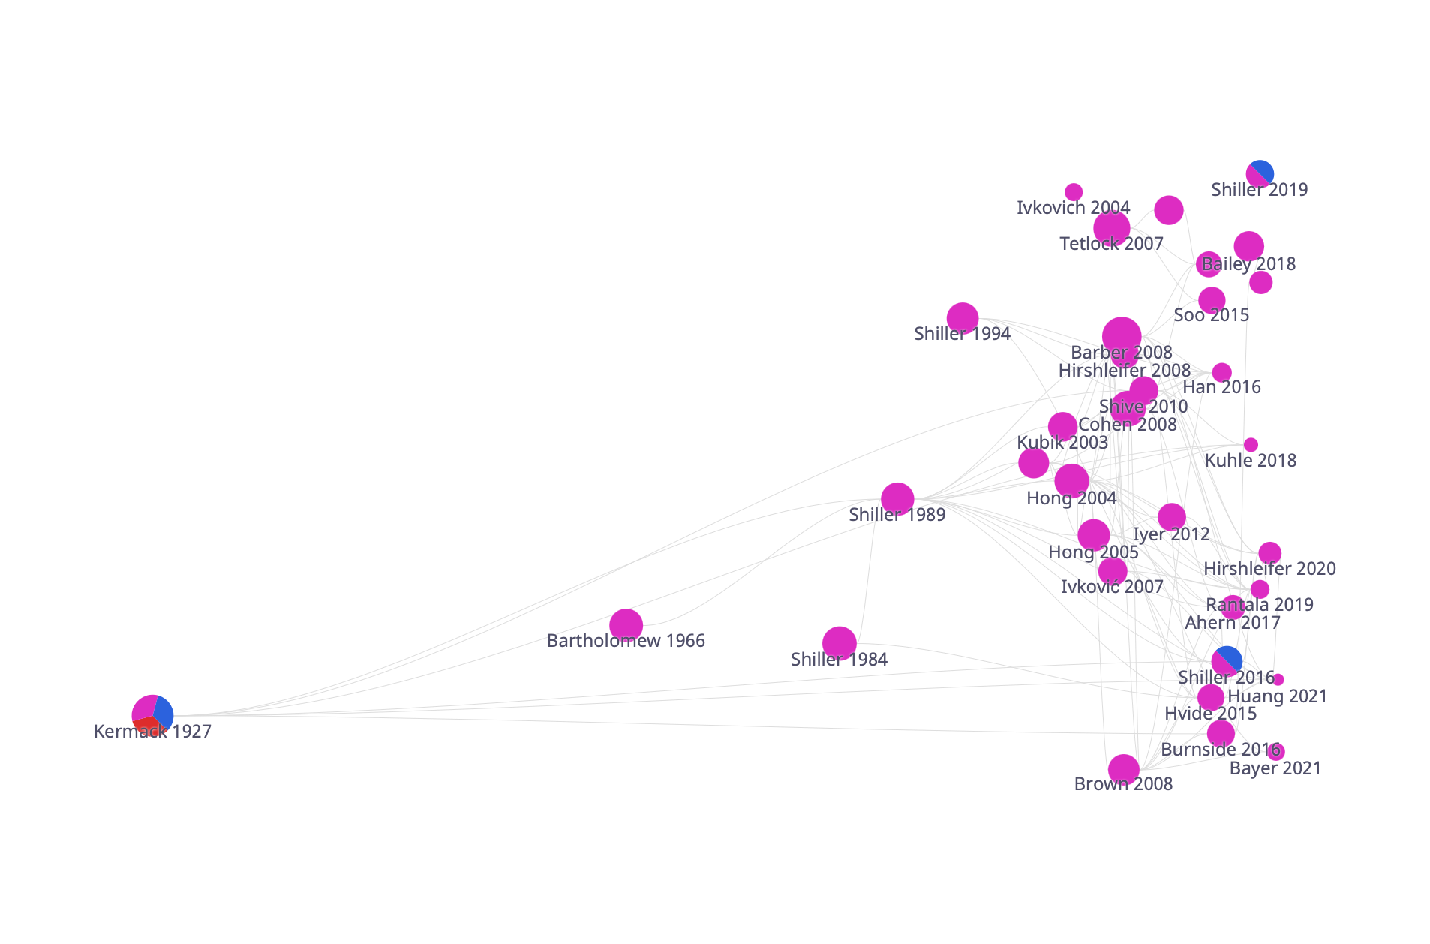
\includegraphics[width=1.5\textwidth]{./figures/graph_investment}
  \begin{flushleft}
    {\footnotesize Note: This graph includes selected papers related to epidemiological models of expectations in asset markets, and studies of the role of news media in financial markets. See \href{https://app.litmaps.co/shared/E25276CA-8725-437B-8241-11961EFB3FB4}{here} for an interactive version.}
  \end{flushleft}
\end{figure}

Academic models of financial markets have traditionally assumed that investors choose stocks based on well-informed rational beliefs about future returns.  But popular treatments have emphasized social communication, and ideas with a distinctly epidemiological flavor, since the first published description of  the first publicly traded securities (\cite{vegaConfusion}'s discussion of the trading of shares of the East India company on the Amsterdam stock exchange).  \cite{mackay1850memoirs}'s vivid prose has made his (thoroughly epidemiological) descriptions of the Dutch Tulip mania and other financial episodes of ``The Madness of Crowds'' a classic of English literature.  This theme has continued to the present: Michael \cite{lewis2011big}'s bestselling book about the Great Financial Crisis goes so far as to suggest that one of the reasons a particular analyst was able to perceive the housing bubble early was his psychological indifference to other people's opinions.

The academic tide seems now to be turning toward an acknowledgment that there is some truth in the popular view. \cite{hirshleifer2020presidential}'s Presidential Address to the American Finance Association urged the profession take up the study of the social transmission of ideas as ``[a] key but underexploited intellectual building block of social economics and finance.''   Hirshleifer specifically points out the potential for epidemiological models to make sense of patterns that have been difficult to understand with traditional models.  \cite{kuchler2021social} propose `social finance' as the name for a field that would study such social interactions, and make a powerful case that new sources of data and new modeling techniques offer great promise.

These are by no means the first academic authors to propose a role for social transmission of financial ideas.  But, as we explained above, the proportion of efforts that could be described as constituting a full-fledged EE analysis, as opposed to piecemeal evidence or provocative theoretical exercises, is small. % (See Figure \ref{fig:graph_investment})

An early example of such a comprehensive approach is the paper by \cite{shiller1989survey} used above to delineate the elements of a standard epidemiological model.  \cite{shiller1989survey} constructed survey questions designed to understand the sources of information that motivated investors' initial interest in the stock that they had most recently purchased (which they designate as `randomly selected' -- \texttt{RAND}).  About a third indicated that their interest in that stock originated with ``a person who is not an investment professional.''  The authors identify another category of stocks owned by their survey respondents as ``rapidly rising'' and for those they find that roughly half of the initial interest in the stock originated with nonprofessionals.  Using a different methodology to designate `rapidly rising' -- `\texttt{RPI}' -- stocks for institutional investors, they find that 10 percent and 30 percent of their initial interest originated from `nonprofessionals.'

The survey-based estimates of their epidemiological model for both individual (`\texttt{IND}') and institutional (`\texttt{INS}') investors reveal considerable heterogeneity in infection rates both within and between the two groups. They also suggest that the infectiousness differs between a randomly selected stock \texttt{RAND} and a rapidly rising stock \texttt{RPI}. Interestingly, they find that the \texttt{RAND} category is more (interpersonally) ``infectious'' than the rapidly rising stock; they propose, plausibly, that public news sources will already have widely covered the rapidly rising stocks, so that interpersonal communications are unnecessary to bring attention to them.

Our Figure \ref{fig:sir_simulate} shows the compositional changes of investors under the paper's median estimates (of infection and removal rates) for individual and for institutional investors, and for randomly selected versus for rising stocks, respectively.\footnote{We convert all the continuous-time rates into discrete-time and from annual to weekly frequency. For instance, the recovery rate estimated from the decaying pattern of the time spent on studying a given stock for INSRPI is $g=1.39$ (a half-life of $ln(2)/g=0.50$ years). In discrete-time and at weekly frequency, this is equivalent to a probability of recovery $\gamma = 1-\exp^{-g/52} =0.02$. For the removal rate, under the assumption made by the paper that the fraction of susceptible is close to $1$ despite being time-varying, the estimated median removal rate of INSRPI is $b = 2.02$. It is converted to a weekly probability of $\beta = 1-\exp^{-b/52}=0.038$.}$^{,}$\footnote{We set the initial fraction of the infected to be $1$ percent.}

% \centerline{[Insert Figure \ref{fig:sir_simulate} here]}

\begin{verbatimwrite}{./Slides/FigureSIRSimulation}%%%Slides
  \begin{figure} \centering  % [h!]  [!ht]
    \caption{ ~Simulated dynamics from a SIR model of stock investors}
    \label{fig:sir_simulate}
    \centerline{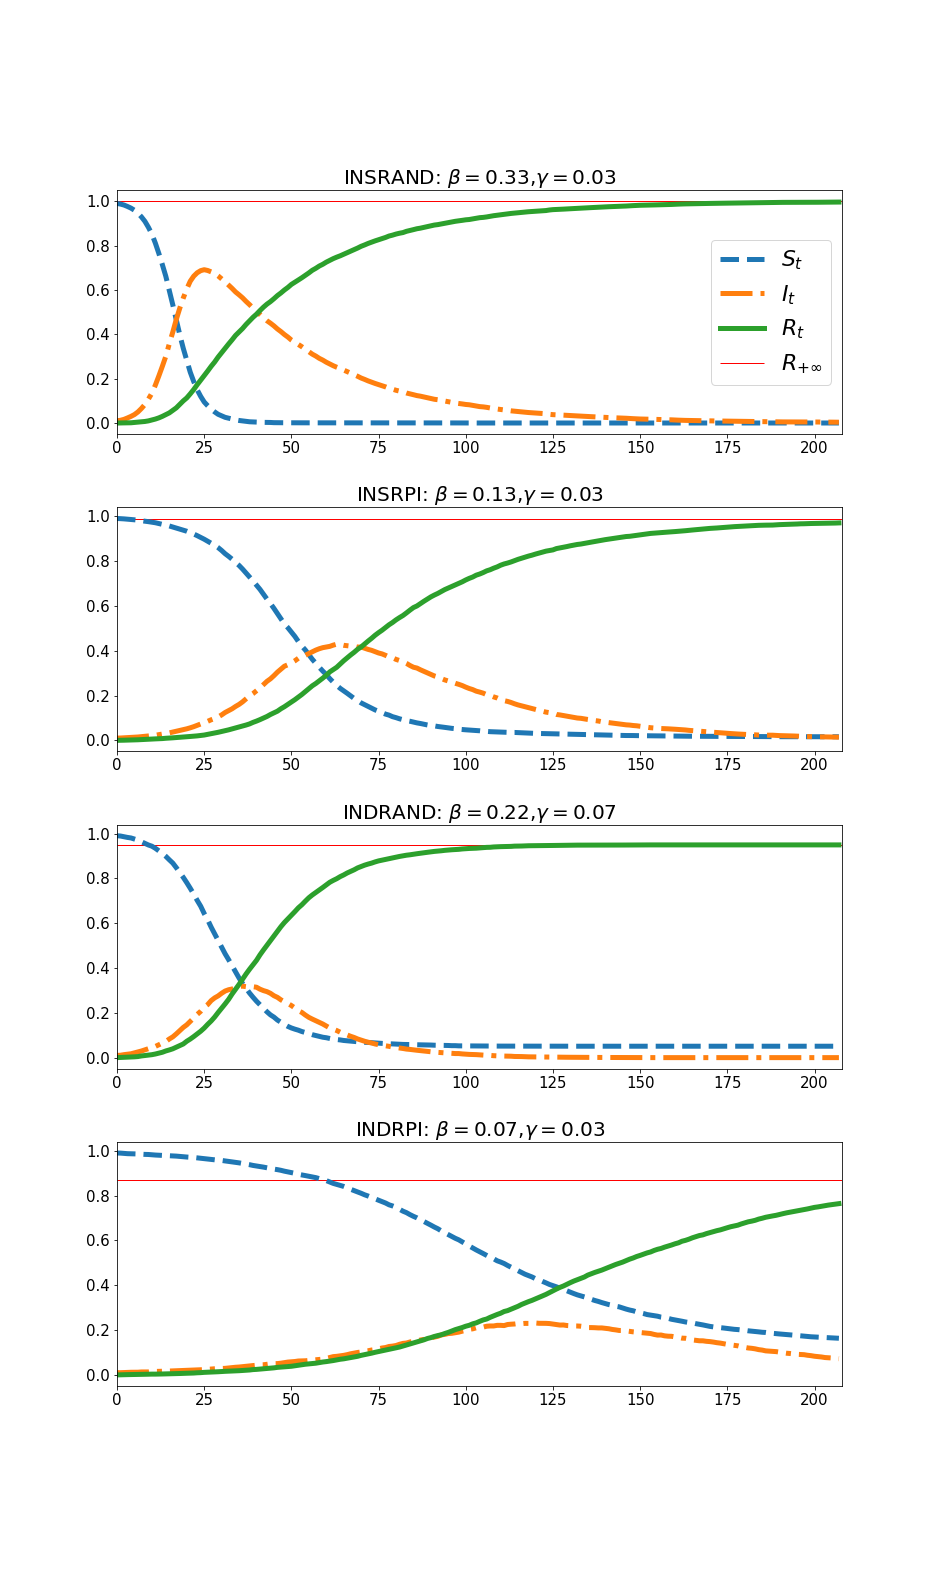
\includegraphics[width=1.2\textwidth,height=1.2\textheight]{./figures/sir_simulate}}
    \begin{flushleft}
      {\footnotesize Note: This graph plots the simulated paths of populations in different compartments in a SIR model of stock investors, as described in \cite{shiller1989survey}. We use the median estimates of the infection rate $\beta$ and recovery rate $\gamma$ for four samples: institutional investors for a randomly selected stock (INSRAND), institutional investors for a rapidly rising stock (INSRPI), individual investors for a random stock (INDRAND), and individual investors for a rapidly rising stock (INDRPI). The horizontal thin solid line corresponds to the limiting size of compartment of $R$ in the long run. The simulation is done with the Python library \href{https://ndlib.readthedocs.io/en/latest/}{``NDlib''}, for details, see the companion \href{https://github.com/llorracc/EpiExp/blob/master/SIR_Ndlib.ipynb}{Jupyter Notebook}. }
    \end{flushleft}
  \end{figure}
\end{verbatimwrite}%%%Slides
%%%Slides
  \begin{figure} \centering  % [h!]  [!ht]
    \caption{ ~Simulated dynamics from an SIR model of stock investors}
    \label{fig:sir_simulate}
    \centerline{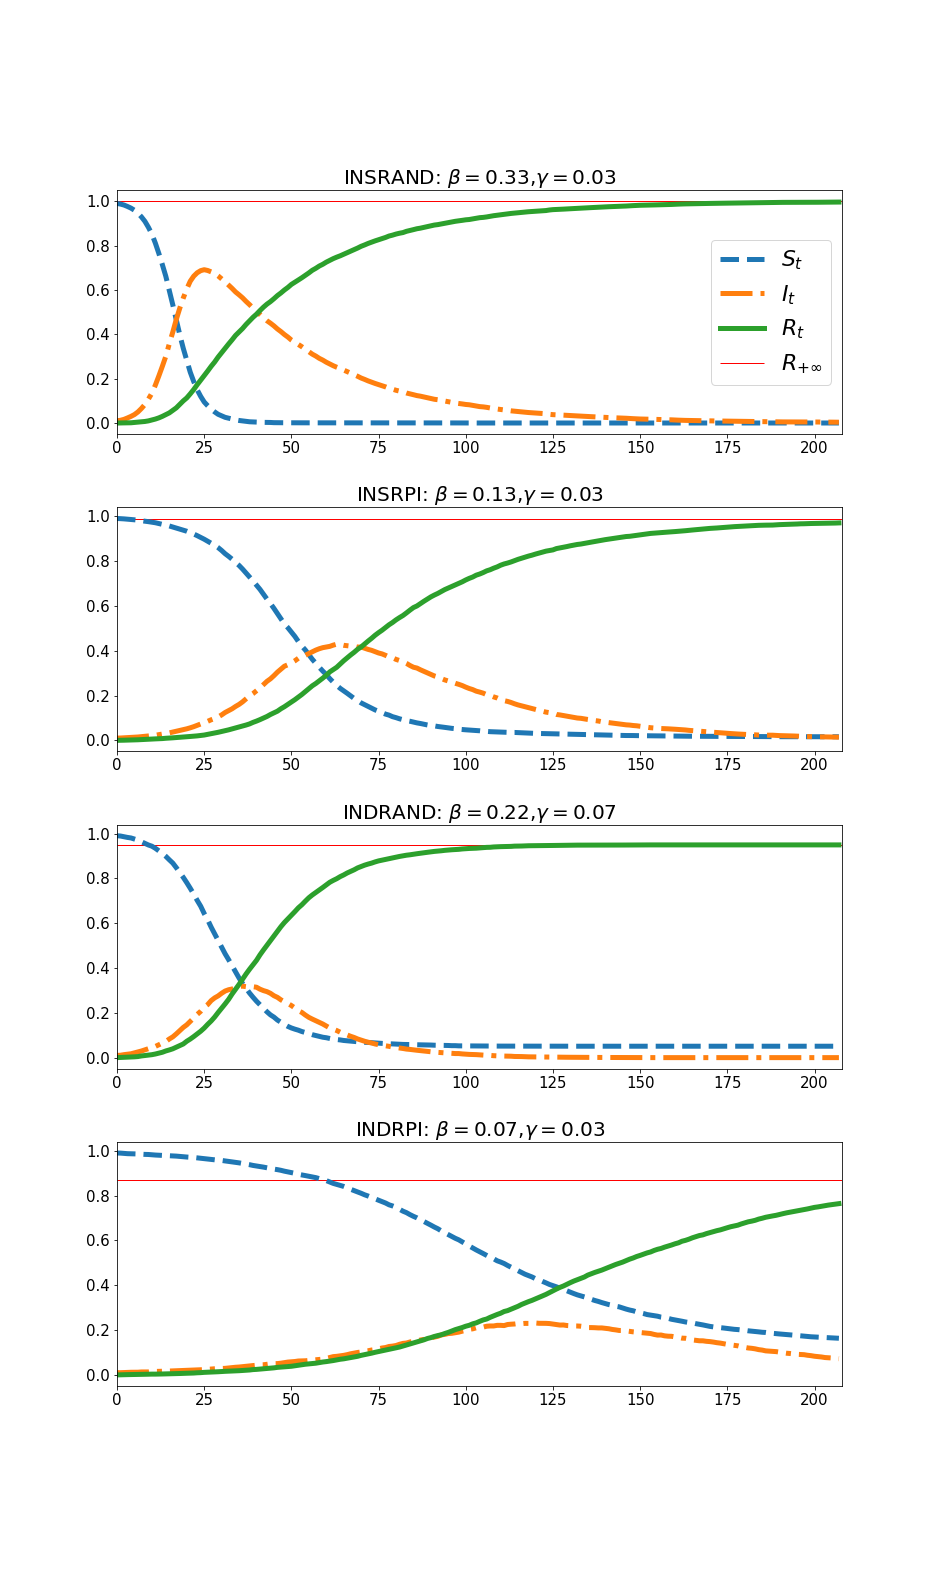
\includegraphics[width=0.85\textwidth,height=0.85\textheight]{./figures/sir_simulate}}
    \begin{flushleft}
      {\footnotesize Note: This graph plots the simulated paths of populations in different compartments in a SIR model of stock investors, as described in \cite{shiller1989survey}. We use the median estimates of the infection rate $\beta$ and recovery rate $\gamma$ for four samples: institutional investors for a randomly selected stock (INSRAND), institutional investors for a rapidly rising stock (INSRPI), individual investors for a random stock (INDRAND), and individual investors for a rapidly rising stock (INDRPI). The horizontal thin solid line corresponds to the limiting size of compartment of $R$ in the long run. The simulation is done with the Python library \href{https://ndlib.readthedocs.io/en/latest/}{``NDlib''}, for details, see the companion \href{https://github.com/llorracc/EpiExp/blob/master/SIR_Ndlib.ipynb}{Jupyter Notebook}. }
    \end{flushleft}
  \end{figure}
%%%Slides

The epidemiological analysis above is for parameters that characterize a sample of highly interested and motivated investors.  There is no sense in which these parameters can be thought of as characterizing the whole population -- which is why it is not as surprising or implausible as it might seem that all the parameterizations of the models were ones in which $\Recovered$ (the proportion of investors who would eventually become interested in a stock) was high.

The economic analysis can now also be interpreted in temporal terms.  The authors point out that a fully rational model with no private information would imply that trading volume should be heavily concentrated around identifiable dates of news events, but the epidemiological model is consistent with long and variable lags.  It takes around half a year for the interest of institutional investors in the randomly selected stocks to reach its peak and a little more than a year for a rapidly rising stock. As for individual investors, the population interested in \texttt{RAND} reaches its peak after 40 weeks, while interest in \texttt{RPI} takes 2.5 years to peak.


% sAlthough such paths correspond to a particular set of configurations, they presumably shed light on the general evolution patterns of stock investors' interests.  For instance, so long as the infection rate is higher than the removal rate, the fraction of infected investors will follow a hump shape  -- because the number of susceptible persons is declining.

The paper also argues that in a special case where the infection rate is close to the removal rate, and the size of the pool of interested investors is driven by serially uncorrelated shocks, stock prices could follow a random walk, because under those assumptions the change in the level of `interest' is nearly unforecastable.\footnote{\cite{shiller1984stock} presents an  elaboration on this logic by allowing the presence of both rational investors (``smart money'') and social-dynamics driven investors. The presence of unforecastable social dynamics weakens the statistical power of the random-walk test of rationality of stock market.} This is another example of an economic consequence flowing from the pattern of spread of an infection.  Furthermore, the pool of investors is potentially measurable, so it is an implication that can be tested.

Remarkably little of the extensive literature citing \cite{shiller1989survey} has involved meaningful epidemiological modeling; almost all of it has either been empirical, or has used a modeling framework that cannot be characterized as `epidemiological' as we are interpreting the term. %in Section \ref{subsec:epi_framework}.

A potential reason for this lack of followup is the nonexistence, until quite recently, of much direct data on either of the two key components of the model: beliefs (about, say, stock prices), or social connections -- and no data at all about the \textit{changes} of beliefs as a function of the structure of a measured social network.  \cite{shiller1989survey} had to make heroic assumptions in order to quantify their model.  Few subsequent scholars seem to have been willing to go so far in employing what might today be termed an `indirect inference' approach: ``Assuming the epidemiological model is right, let's calibrate it using its downstream implications for things we can observe.''

However, we have found two good exceptions, both of which estimate parameters of structural epidemiological model of stock investors using microdata.

The first is  \href{https://github.com/iworld1991/EpiExp/blob/master/Literature/shive2010epidemic.pdf}{\cite{shive2010epidemic}}, which uses an SI (`susceptible-infected') model to inform the structure of a reduced-form regressor that aims to capture social influences among investors.  Using nearly the universe of ownership data for Finnish stocks between 1994 and 2004, the author assumes that the key social infection channels are at the municipal level, and estimates the time-series dynamics of ownership within municipalities.

Specifically, controlling for all of the variables (demographic variables, news sources, price dynamics, and others) that standard models might suggest could affect ownership patterns, the author estimates an equation that can be interpreted as measuring the $\beta$ coefficient in Equation~\eqref{eq:sirdyn}.  The estimated $\beta$ coefficient is highly statistically significant, indicating at a minimum that there is some local dynamic pattern to stock purchases not captured by the usual finance and economic models, but which is captured by `proportion locally infected last period' (corresponding to $S_t/N$ in Equation~\eqref{eq:sirdyn}).  % An epidemiological interpretation of this fact seems quite natural.

The second example is \href{https://github.com/iworld1991/EpiExp/blob/master/Literature/huang2021rate.pdf}{ \cite{huang2021rate}}, which estimates an epidemiological model of diffusion of financial news among geographical neighbors. The paper reports a time-average estimate of the reproduction ratio $\mathcal{R}$ between $0.3$ to $0.4$ (equivalent to $\frac{\beta S_t/N}{\gamma}$ in an SIR model); that is, each stock trade that the authors identify as exogenous (see the paper for the mechanism) resulted in a total of $0.3{\sim}0.4$ trades among that person's neighbors, aggregated over all neighbors and all time.

The authors also find stronger transmission between investors of the same characteristics (age, income category, and gender), confirming the usual presumption of homophily (people tend to trust others with similar backgrounds). The paper found stronger transmission between senders and receivers with high past performance, suggesting that conversations between neighbors were more likely when past performance has been high.  The natural interpretation -- consistent with common findings in behavioral finance -- is that you are more likely to boast about your investment in a winner than admit to having invested in a loser.

Their estimate that $\mathcal{R}$ is positive and highly statistically significant is consistent with the presence of neighborly social influence, and they work hard to rule out plausible alternatives. But since the estimated reproduction ratio is below  1, their results imply that news of this kind does not lead to an epidemic of stock trading.  This is in contrast with \cite{shiller1989survey}, whose corresponding reproduction ratios far exceeded one.  This difference highlights the extent to which epidemiological models must be interpreted with care; even if similar phenomena (stock trading) are being studied, and even if there is evidence of social communication, the estimated nature and size of the epidemiological consequences can vary greatly depending on the exact experiment.

A final, and very impressive, contribution that satisfies all our criteria is a model of housing market fluctuations by \href{https://www.journals.uchicago.edu/doi/abs/10.1086/686732}{\cite{burnside_understanding_2016}}, which shows how incorporating social interactions can generate booms and busts. In the model, agents differ in their beliefs (optimistic or skeptical) about the fundamental value of housing.  Although it is a random-mixing model, paper has a mechanism similar in its implications to the simplest epidemiological model of `super-spreaders' which occurs when some agents have many more social connections than others:  The agents in this model differ in the degree of confidence they have in their opinions (whether optimistic or pessimistic) and those with greater confidence are more likely to convert those who have less confidence.  Defining a `boom' as a period in which house prices rise rapidly as the result of a spread in optimism, and a `bust' as a rapid decline in prices caused by rising proportion of skepticism, their most interesting result is that whether a boom is followed by a bust can depend on whose opinion (optimists or skeptics) turns out to be closer to the true fundamental value.  Specifically, busts happen when the skeptics turn out to be right about the fundamentals, while booms caused by optimists who happen to be right are not followed by busts.

One further literature that deserves a brief mention is the work on ``Agent Based Computational Finance'' (see the survey of that title by~\cite{lebaronAgentCompFinance}).  It would be straightforward to reinterpret much of the work in that literature as exploring epidemiological models of expectations of asset prices and financial market outcomes, and epidemiological terminology is sometimes explicitly invoked in the literature.  Economists interested in constructing formal EE models would do well to delve into that literature for ideas that could be reinterpreted (or relabeled) to purpose.  We have chosen not to survey that literature here partly because there are a number of excellent surveys already available, and in part because that literature has not mainly interpreted itself as modeling the dynamics of expectations.    % by Tao
\subsection{Macroeconomic Expectations}\label{subsec:macroExp}

We have identified only a few papers in macroeconomics (excluding finance; see above) that either constitute full-fledged EE modeling exercises or are closely related to such models.\footnote{See \dmwinflationexpectationFull, and \bvbayesianlearningFull, for non-social models of macroeconomic expectations formation.} \ifInBook{}{Figure~\ref{fig:graph_macro} depicts the network of citation connections between those papers.}

\ifInBook{}{ % don't show these maps for book chapter
\begin{figure}[!ht] \centering  % [h!]
	%\hypertarget{graphmacro}{}
	\caption{ ~Literature map of EE models of macroeconomic expectations}
	\label{fig:graph_macro}
	\centerline{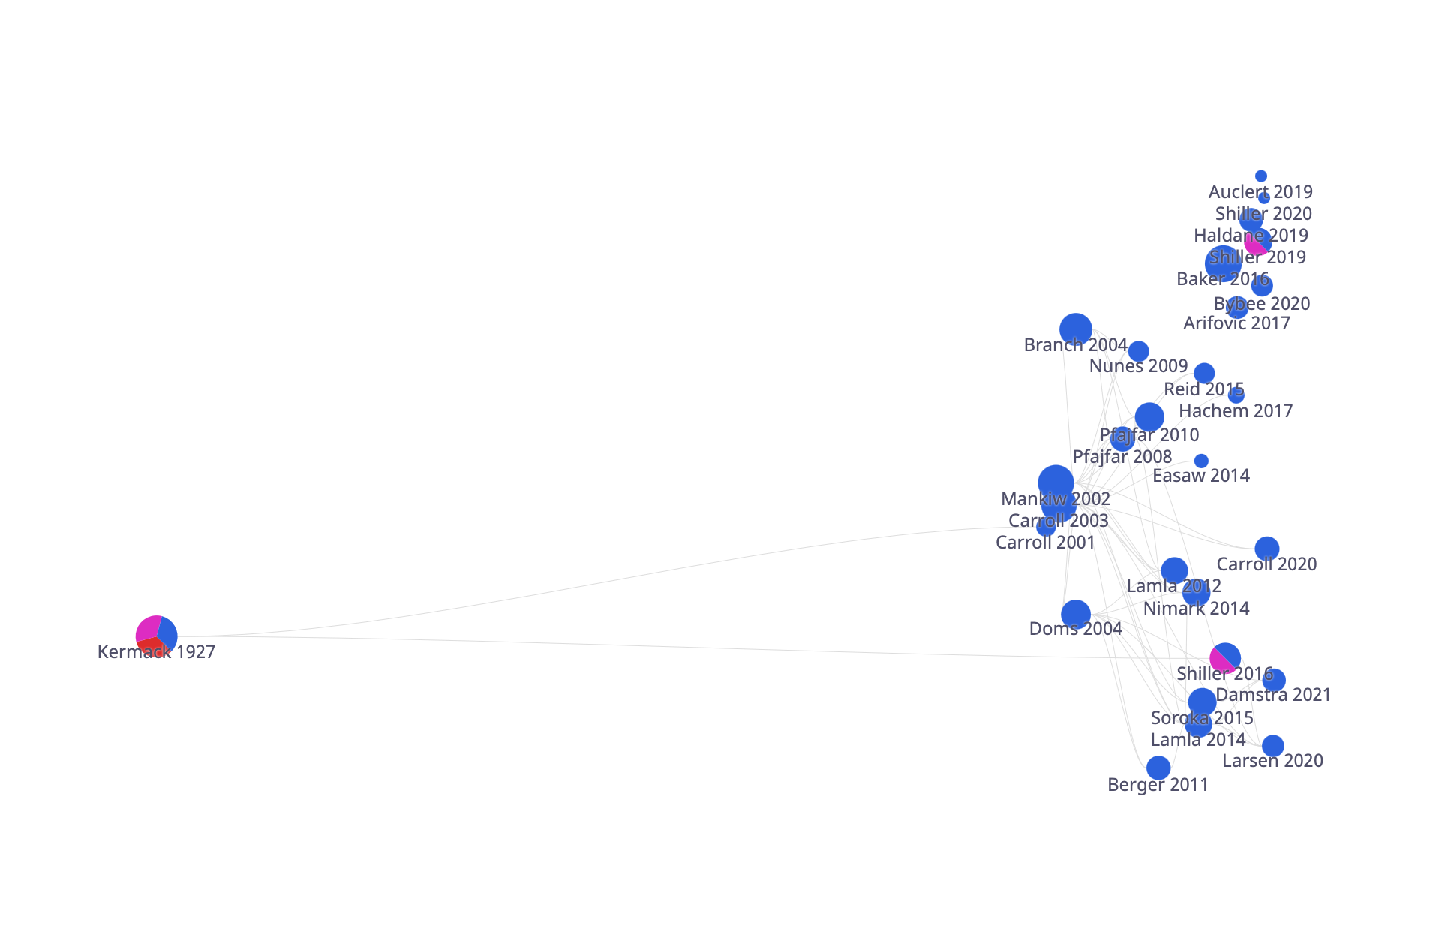
\includegraphics[width=\textwidth]{./figures/graph_macro}}
	\begin{flushleft}
		{\footnotesize Note: This graph includes selected papers related to epidemiological models of macroeconomic expectations, and research on the interaction between news media and macroeconomic expectations. See \href{https://app.litmaps.co/shared/289F57F4-FDE5-4F94-B1A9-2BA7419DB719}{here} for its interactive version.}
	\end{flushleft}
\end{figure}
}

\subsubsection{Sticky Expectations}
%\noindent\textit{\textbf{Sticky Expectations of Inflation}}

%\noindent\cite{mr2002Sticky}-\cite{carroll2003macroeconomic}: Taken in combination, these two papers comprise a framework that satisfies our criteria of a full-fledged EE macroeconomic model -- though neither paper alone would qualify.

%\textit{Sticky Expectations.}

\cite{carroll2003macroeconomic} presents an epidemiological model in which the dynamics of aggregate consumer inflation expectations follow a `sticky expectations' equation:
    \begin{align}
        M_{t}[\pi_{t+1}] & = (1-\lambda)M_{t-1}[\pi_{t}]+\lambda \mathbb{E}_{t}[\pi_{t+1}] \label{eq:StickyExp}
    \end{align}
where $M_{t}[\pi_{t+1}]$ reflects mean consumer expectations at date $t$ for inflation at date $t+1$, and $\mathbb{E}_{t}[\pi_{t+1}]$ is a `rational' expectation with which an individual consumer might be infected.

%\cite{carroll2003macroeconomic} fails the last of our criteria above for a full-bore EE macroeconomic model because he does not work out the consequences of the epidemiological model for macroeconomic dynamics, and \cite{mr2002Sticky} do not present an epidemiological model at all.  But \cite{carroll2003macroeconomic} is effectively an epidemiological microfoundation for \cite{mr2002Sticky}'s key expectational equation, which causes all the deviations of their results from a standard NK model.

%It may be useful here to sketch the key ingredients of the framework, to provide another fleshed-out example of how a simple epidemiological model can be constructed.

This analytical solution for aggregate dynamics of expectations is possible because the paper employs the simplest tool in the epidemiological toolkit: the common-source susceptible-infected (SI) model whose dynamics we presented in table~\ref{table:SIDyn}.\footnote{See~\cite{easaw2015households} for a version that adds social learning between households.}  The idea is that consumers' expectations of inflation stem from exposure to (common) news media sources.  \ifInBook{}{The elements of the framework are:
\begin{quote}
    \normalfont
\begin{enumerate}
    \item All news outlets report professional forecasters' consensus views\footnote{\cite{carroll2003macroeconomic} quotes news stories quoting professionals, and subsequent research by~\cite{lamla2014role} has confirmed the point.}
%    \item Consumers and forecasters believe the same `true' inflation stochastic process
%    \begin{itemize}
%        \item It has purely transitory and purely permanent components
%        \item Shocks to those components are unpredictable
%    \end{itemize}
    \item All consumers are susceptible to infection with probability $\lambda$
    \item Infection means that the consumer adopts the view in the media
    \item The consumer retains that view until next infected
\end{enumerate}
\end{quote}
}
The consequence is a population distribution of beliefs in which a proportion of the population $(1-\lambda)^{n}$ holds the belief previously held by professional forecasters $n$ periods in the past.   \ifInBook{The model }{
The model was also constructed in the manner suggested in~Section~\ref{motivation-and-context}: It} collapses to the rational expectations model as the parameter $\lambda$ approaches 1, making it easy to examine the consequences of the epidemiological deviation from RE.  \ifInBook{}{The model can also be interpreted as nesting the `Rational Inattention' framework, to the extent that one further assumption seems plausible:  Beliefs about inflation derive from exposure to news coverage because the `reading the newspaper' method of becoming informed is almost infinitely easier than solving (yourself) the full-fledged Rational Inattention macroeconomic model.\footnote{It is perhaps plausible to model the professional forecasters themselves as having the skills and time and motivation to solve the full Rational Inattention model - or, alternatively, an EE model.}}

Another implication -- inflation expectations are a result of the degree of exposure to news stories -- leads to a straightforward prediction:  The speed at which inflation expectations move toward professionals' expectations will depend on the intensity of news coverage of inflation.  \cite{carroll2003macroeconomic} found some support for this; \cite{lamla2014role} and \cite{larsen2021news} find further evidence that a greater intensity of news coverage of inflation leads to more accurate expectations in the population.  % CDC: we should cite this:  More recently,  identified topics discussed in the news media related to inflation using machine learning algorithms and found they are good predictions of inflation expectations. The intensity of inflation-related topics in the news media accounts for the time-varying rigidity in information, as predicted in the model.


% For slides: These results may be of some interest at the present moment when news coverage about inflation is intense.  But another result from the paper is also interesting: An explicit horserace was done between a version of the model in which consumers' views adjusted toward the most recently reported actual inflation statistic, versus adjusting toward professional forecasters predictions of future inflation.

%\noindent\textit{Sticky Information.}

The SI model provides a plausible (and testable) microfoundataion for the work of \cite{mr2002Sticky}, who simply assume that the dynamics of inflation expectations are given by a process like \eqref{eq:StickyExp}; they call this a `sticky information' assumption,\footnote{See \bvbayesianlearningFull  for an alternative potential microfoundation.} and argue that the macroeconomic implications of a New Keynesian model in which expectations work this way match a variety of facts (most notably, the sluggishness of inflation dynamics) that standard NK models cannot capture.  \cite{mankiw2007sticky} extend the analysis of their earlier paper to a general equilibrium context with goods, labor, and financial markets, and point out explicitly that the stickiness that drives the core results in their new model can be motivated by an epidemiological model.

%\ifInBook{}{The combination of their paper with that of~\cite{carroll2003macroeconomic} is closer to constituting a full-fledged EE approach to macroeconomic modeling than either paper is alone: Carroll's paper did not examine the consequences of his model of inflation expectations for anything else, while \cite{mr2002Sticky} did not provide a microfoundation for their `sticky information' equation.  (Conveniently, however, their baseline calibration of the model was $\lambda=0.25$, while Carroll's empirical estimate of the parameter was $0.27$.)\footnote{A number of subsequent papers have estimated similar equations in a variety of countries, generally finding roughly similar results.}}

An example closely related to the overtly epidemiological work on inflation expectations is \cite{branchHeteroExp}, who considers a model in which agents who have different inflation forecasting rules meet each other and the rules that work better are adopted.

\begin{comment}
\subsubsection{Effectiveness of Monetary Policy}

Heterogeneous expectations have important implications for the effectiveness of central bank communication.   To capture this point, \cite{hachem_inflation_2017} construct a model in which monopolistically competitive firms hold heterogeneous inflation expectations due to different forecasting rules. One group of firms simply expect inflation to remain stable (``Random Walkers''), and the other group makes forecasts based on central bank announcements (``Fed Watchers''). The fraction of Fed Watchers summarizes the credibility of the central bank.  The model's epidemiological content comes from the transmission of beliefs about which strategies to pursue:  firms meet each other and potentially switch forecasting rules based on relative performance. The paper shows that for the central bank, a period of gradual announcements helps build credibility and achieves target inflation, while an abrupt change in the target leads to undershooting.
\end{comment}

%\subsubsection{Sticky Consumption}

A number of recent papers including \cite{shibata2019current}, \cite{carroll2020sticky}, and \cite{auclert2020micro} have applied the same SI epidemiological model used in \cite{carroll2003macroeconomic} to model the behavior of consumers whose attention to macroeconomic news may be spotty even if they are very well informed about their own idiosyncratic circumstances.  The consequence is that aggregate consumption exhibits `excess smoothness' in a way that matches macro data well, while at the same time predictions about microeconomic behavior are consistent with the micro facts that have been used to discipline the new generation of HA-Macro models.

%One advantage of the consumption context over that of inflation is that consumers have a utility function that can be used to calculate the cost of deviations from instantaneous and perfect updating.  When the `news infectiousness' parameter is calibrated so that the model's consumption dynamics match aggregate consumption dynamics, the cost to consumers of failing to read every news story (alternatively, of the `infectiousness' of news being less than 100 percent) is negligible.  This is because the vast majority of the uncertainty consumers face stems from idiosyncratic, not aggregate, risks, so being a little bit out of date with respect to the latest aggregate developments has only a very small cost.

\subsubsection{Sentiment and the Business Cycle}

Section \ref{subsec:microEvidence} summarizes evidence of macroeconomic effects of consumer sentiment or ``animal spirits.''  Most of the theoretical work in this area\footnote{For example, \cite{angeletos2010noisy}, \cite{benhabib2015sentiments}, \cite{angeletos2018quantifying}.}  resembles the theoretical work in on financial contagion:  It examines questions like existence of an equilibrium (or multiple equilibria), but does not focus on understanding social interaction mechanisms by which the equilibrium could come about, and does not use expectations data to test the model.

\cite{angeletos2013sentiments} is an exception.  It rationalizes sentiment-driven business cycle fluctuations with a theoretical model with an explicit epidemiological mechanism. The paper defines the ``sentiment shocks'' as extrinsic belief shocks that neither affect fundamentals (such as technology and preferences) nor the beliefs about these fundamentals and shows that these shocks still drive equilibrium outcomes under the critical assumption that imperfect communication prevents agents from achieving common knowledge.  The paper explores aggregate belief and output dynamics after an exogenous sentiment shock hits a fraction of agents and gradually spreads via random mixing.  The paper computes  population flows between what an epidemiologist would describe as three `compartments' (uninformed, informed, and fully informed about productivity). Such dynamics induce ``fad-like'' or boom-bust dynamics of both aggregate beliefs and realized outputs.


\subsubsection{Learning of Macroeconomic Equilibria}

% TW to CDC: \cite{han2019visibility} can be cited here.

\ifInBook{}{The presence of social influences on agents' expectations also has an aggregate saving/consumption impact.  For instance, without complete information about the state of the economy or future income prospects, agents in the economy may form expectations via observing the consumption of others. In such a context, \cite{han2019visibility} utilizes a sensible daily observation that usually the consumption of others tends to be more salient than their savings (what the author called ``visibility bias'') to explain the well-known macroeconomic phenomenon of under-saving by households. When the agents fail to take into account the asymmetry between signals from consumption and non-signals from saving of others in the learning process, they hence form upward biased income expectation on average, which leads to over-consumption in the equilibrium. It is worth noting that such a mechanism works particularly through the expectation of agents instead of via preference-dependence, a la the ``catching up with the Joneses'' effect. The authors also argue that the secular penetration of communication technology might have been a contributing force to the decline of the saving rate of the United States since the 1980s, as it intensified the visibility bias of consumption.}

\cite{brock1997rational} model the dynamics of beliefs using a model in which there is a population of forecasting rules that agents can adopt, and in which the agents periodically construct a predictor by choosing combinatoins of forecasting rules whose performance has been better.  The dynamics in the model are described as reflecting the `survival of the fittest.' \cite{arifovic2018learning} also examine an economy with agents who have different macroeconomic forecasting rules.  Aggregate dynamics evolve as agents discard their own rules when they encounter other agents whose rules have proven more effective.  Another way of describing this would be to say that more effective rules are more infectious.   \ifInBook{}{Indeed, the parallel to the biological process is deeper: As diseases can do, the rules can mutate into more (or less) effective forms.}  The paper also discusses the potential role of professional forecasters and the extent to which their views can spread to the population at large -- in our terminology, because their views are more `viral.'

These papers are examples of an `agent-based modeling' approach, which \cite{tesfatsion2006agent} has argued has application to many subfields of economics.  \cite{haldane_drawing_2019} make a strong case for a broad reinterpretation of these kinds of models as epidemiological, particularly in the macroeconomic context.  Though most such models do not use expectations data to test their implications (an exception is the work of~\cite{hommes2006heterogeneous}; see also \cite{branchHeteroExp}), it is a short leap from the assumption that successful decision rules spread to an interpretation that what spreads is a set of expectations that would induce the decision rule that is spreading.

As with the work on agent based modeling in finance, we chose not to attempt a summary of this literature because excellent comprehensive surveys already exist (see, e.g., \cite{ddAgentBasedMacro}).  But readers interested in these subjects would do well to absorb this literature (and especially the work of Hommes).

\begin{comment}
\subsubsection{Other Work}

Among our criteria for narrowing the scope of what constitutes a `full-fledged' EE modeling approach, the most effective was our requirement that the expectation dynamic have a clear connection to some separately measurable economic outcome.

Because expectations of inflation (or of other variables) are so widely believed (by economists, at least) to be a driver of actual inflation outcomes, we have permitted ourselves to include models that measure themselves by their success in explaining the movements in surveyed expectations.

But that leap does require belief in a connection between measured beliefs and actual choices

One question that might arise is whether news coverage is a plausible driver of actual consumer behavior.  Several papers have found evidence that news coverage does have substantial impact on households' beliefs about economic matters.  A clever paper by \cite{doms2004consumer} shows that consumer sentiment is driven by news coverage even during periods in which coverage is inconsistent with economic conditions.  (They cite an extensive prior literature that has found evidence that consumer sentiment itself is correlated with economic choices in ways not captured by other observable macroeconomic variables).\footnote{For further evidence that news coverage is a key source of people's views, see \cite{lamla2012role}, though see~\cite{pfajfar2013news} for a skeptical view.  }


\begin{itemize}
	\item \cite{carroll2003macroeconomic}, \href{http://www.econ2.jhu.edu/people/ccarroll/epidemiologySFI.pdf}{\cite{carroll2005epidemiology}}: ``rational'' forecasts by professionals spread to average households as in a common source epi model
	\begin{itemize}
		\item insights:  arguably simplest model that could be interpreted as ``epidemiological''
		\item mechanism:
		\begin{itemize}
			\item
			ordinary people: exposed, at constant rate, to news media which reports what ``experts'' say
			\item
			fraction of people who absorb those views depends on ``infectiousness'' of experts' views
			\item $\Rightarrow$ population beliefs are geometric lag of experts' beliefs
			\item
			embeds RE model as the limit corresponding to ``infinitely instantly
			perfectly infectious'' beliefs
		\end{itemize}
		\item implications:
		\begin{itemize}
			\item
			stickiness of aggregate expectations: most recent economic news \href{http://www.econ2.jhu.edu/people/ccarroll/epidemiologySFI.pdf}{\cite{carroll2005epidemiology}}, \href{http://www.econ2.jhu.edu/people/ccarroll/epidemiologyQJE.pdf}{\cite{carroll2003macroeconomic}} and policy annoucements  \href{https://www.tcd.ie/Economics/staff/waltis/EC2010/ec2010_ps5ans.pdf}{\cite{berger2011monetary}} do not reach to all private agents instantaneously
			\item aggregated sluggishness in adjustment in shock responses, i.e. consumption \href{https://www.ecb.europa.eu/pub/pdf/scpwps/ecb.wp2152.en.pdf}{\cite{carroll2020sticky}},  \href{https://www.nber.org/papers/w26647}{\cite{auclert2020micro}};
			\item
			which affects what Fed governors and treasury secretaries do, e.g. central bank communication
		\end{itemize}
	\end{itemize}

	\item \cite{doms2004consumer}:  consumer sentiment driven by news coverage even during periods in which news coverage is inconsistent with economic conditions.
	\item \href{https://github.com/iworld1991/EpiExp/blob/master/Literature/lamla2012role.pdf}{\cite{lamla2012role}}: disagreement of households depends on the heterogeneity of story contentand on the reporting intensity, especially of news on rising inflation. Disagreement of professional forecasters does not depend on media coverage. % MICHAEL J. LAMLA THOMAS MAAG The Role of Media for Inflation Forecast Disagreement of Households and Professional Forecasters This paper investigates the effects of media coverage about consumer price inflation on inflation forecast disagreement of German households and pro-fessional forecasters. We adopt a Bayesian learning model in which mediacoverage of inflation affects forecast disagreement by influencing infor-mation sets as well as predictor choice. Our empirical results show that disagreement of households depends on the heterogeneity of story contentand on the reporting intensity, especially of news on rising inflation. Dis-agreement of professional forecasters does not depend on media coverage.With respect to the influence of macroeconomic variables, we provide ev-idence that disagreement of professional forecasters primarily depends onthe inflation rate and on inflation volatility. The response of households toinflation is much less pronounced.
	\item \href{https://github.com/iworld1991/EpiExp/blob/master/Literature/pfajfar_news_2013.pdf}{\cite{pfajfar_news_2013}}: tests the epidemiological model using directly reported news exposure in the Michigan Survey(``news heard about aggregate price changes''(available since 1961)) and finds that recent news exposure does not lead to more accurate forecasts. Most of the households seem to not adjust beliefs toward recent professional forecasts. The authors attribute this to distorted information reported in the news in the first place.    %Specifically, the following question is addressed to each household "During the last few months, have you heard of any favorable or unfain business conditions?"12 In case of an affirmative response, a second question is asked: "What did you hear?" To address this query, the respondent is presented with a number of options regarding the type of business conditions she might have heard about, such as government, unemployment, prices, consumer demand, stock market, credit, and trade deficit. She is allowed to name at most two of these options. Should prices be one of the selected options, she can reply either (i) "Favorable News: Lower Prices" or (ii) "Unfavorable News: Higher Prices.

	%"Moreover, it appears that households do not make the best use of the information they perceive, as they persistently deviate from professional forecasters' mean expectation, displaying no tendency to adjust their forecasts appropriat. One possible interpretation is that news transmitted by the media distorts consumers' expectations, as it may contain judgmental assess ments of professional forecasters' views. As a consequence, media reports could be biased and the epidemiological mechanism results as a channel that transmits dis torted expectations. This factor could also explain why the degree of perception of unfavorable news on prices is significantly higher than that of favorable news, and why the accuracy of consumers' expectations decreases in the volume of negative news being perceiv"
	% A link to michigan survey on news heard about prices https://data.sca.isr.umich.edu/get-chart.php?y=2021&m=1&n=23h&d=ylch&f=pdf&k=ce35d9fed5ce19c35c089331bd03e10e68f96c690f6bac22c6a77be0beda6204

	\item \href{http://www.sarah-lein.ch/pdfs/inflationexpectations.pdf}{\cite{lamla2014role}}:  the intensity of media reporting of inflation leads to forecast accuracy while the content may bias the inflation expectations.  It augments \cite{carroll2003macroeconomic} with Bayesian learning at individual level admitting bias from the media. %This paper analyzes the impact of the media on consumers’ inflation expectations. We distinguish between two channels through which the media can influence expectations. First, the intensity of the coverage of inflation reports plays a role (volume channel). Second, the content of media reports have an effect (tone channel). Employing a detailed data set capturing media reports on inflation in Germany during the period comprising 01/1998-09/2007, we are able to discriminate between these two effects. We find that the volume effect improves the accuracy of consumers’ forecasts, whereas the tone channel may bias inflation expectations
	\item \href{https://github.com/iworld1991/EpiExp/blob/master/Literature/hachem_inflation_2017.pdf}{\cite{hachem_inflation_2017}}:  the effectiveness of central bank announcements when firms have heterogeneous inflation expectations a la \cite{carroll2003macroeconomic}.
	\item These work suggest that the canonical common-source epidemiological model can be enriched to be reflect the differences in the sources of the infection(news media, professional forecasts, or statistical agencies, etc) and the belief updating rule by households(Bayesian signal extraction or naive updating, etc) can be useful to match macroeconomic expectation dynamics.
\end{itemize}

\end{comment}
  % by Chris
% \subsection{Related Work}
\subsection{Nonstructural Empirical Evidence}\label{subsec:microEvidence}


% \subsubsection{Background}

Above we cite efforts to construct and calibrate structural models of epidemiological models.  %But our definition of an epidemiological process as one in which social interactions affect people's beliefs and consequent economic behaviors means .
Here, we touch upon literatures that collect evidence in ways not targeted to constructing structural models, but that may nevertheless be useful in guiding the construction of structural EE models.

\begin{verbatimwrite}{./Slides/MicroEvidence}
  \begin{enumerate}
  \item When do socially transmitted beliefs influence important economic decisions?
  \item What are characteristics of sources and recipients of expectational infection?
  \item Through which channels are expectations mostly transmitted?
  \item What kinds of information/expectations are more infectious?
  \item How can \cite{manski1993identification}'s reflection problem be addressed?
  \end{enumerate}
\end{verbatimwrite}

\ifthenelse{\boolean{inBook}}{}{Such work could help answer questions like
  \begin{quote}
    \normalfont
      \begin{enumerate}
  \item When do socially transmitted beliefs influence important economic decisions?
  \item What are characteristics of sources and recipients of expectational infection?
  \item Through which channels are expectations mostly transmitted?
  \item What kinds of information/expectations are more infectious?
  \item How can \cite{manski1993identification}'s reflection problem be addressed?
  \end{enumerate}

  \end{quote}

  Among the reasons epidemiological modeling has been slow to spread,  surely one is that all of these questions is difficult to answer using traditional data sources.  But new data, particularly the social network data, offer rich opportunities for improving our ability to answer such questions.
}

\subsubsection{Directly Measured Social Networks}\label{subsubsec:socialnetworks}

Direct data on social interactions have only very recently become available to researchers.  One of the first papers to use such data is \cite{allen2018social}, who use data from peer-to-peer (P2P) FinTech platforms to examine effects of social connections on consumer and small business loans.  They find that P2P loan demand in a given locale increases faster it has previously been growing in its socially connected locales, even when they are geographically distant.  \cite{cookson_why_2020} use data from a social media investing platform to examine sources of disagreement across investors who are in direct communication with each other.

Several papers have used data from Facebook.  \href{https://www.journals.uchicago.edu/doi/abs/10.1086/700073}{\cite{bailey2018economic,bailey2019house}}, using data on individual users' social networks, show that people who happen randomly to have social-network friends in distant cities where home prices have increased are more optimistic about their local housing market, and more likely to buy, than people whose remote friends happen to live in places where house prices declined.\footnote{See \kpshousingexpectationFull, for a discussion of various drivers of housing price expectations.}

\cite{bailey_social_2018} constructed an aggregated social-connectedness-index (SCI)  using the universe of Facebook users, which calculates the Facebook connections between any two zip codes in the U.S., as well as the connections of each zip with foreign countries.  There is already a burgeoning literature using these data (much of it outside of economics).  Among selected early results in economics, \cite{makridis2019effect} shows that a rise in a locality's sentiment caused by events in socially connected areas has a substantial effect on nondurables spending.  \cite{makridis2020learning} find that during the COVID-19 crisis, the severity of the decline in consumption in a county was partly explained by the severity of the epidemic in the places to which that county had especially dense social ties -- even when those places were geographically distant.
\cite{ratnadiwakara2021flooded} shows that individuals who are socially connected to someone affected by Hurricane Harvey are more likely to purchase flood insurance policies after the event. %This effect is stronger in areas at higher risk of flooding. Being socially connected to someone affected by Hurricane Harvey also influences individuals' perceptions of global warming.

% Word-of-mouth communications might be even particularly important in spreading the information in fraudulent contagion and speculative investment activities. For instance, \href{https://github.com/iworld1991/EpiExp/blob/master/Literature/rantala2019investment.pdf}{\cite{rantala2019investment}} provides direct evidence on diffusion of investment ideas among a large Ponzi scheme. \href{https://files.fisher.osu.edu/department-finance/public/information_networks_evidence_from_illegal_insider_trading_tips.pdf}{\cite{ahern2017information}}shed light on the information flow of illegal insider trading among strong social ties.

\subsubsection{Papers Using Proxies for Social Connections}

In the absence (until very recently) of direct evidence about the nature and frequency of social contacts between people, economists have naturally used proxies.    \href{http://www.columbia.edu/~hh2679/ThyNeighborJF.pdf}{\cite{hong2005thy}} found that fund managers tend to buy similar stocks to other fund managers in the same city. \href{https://github.com/iworld1991/EpiExp/blob/master/Literature/hvide2015social.pdf}{\cite{hvide2015social}} found that a person's stock market investment decisions are positively correlated with those of coworkers.  \href{https://www.jstor.org/stable/10.1086/592415}{\cite{cohen2008small}} show that fund managers place larger bets (that perform better) on firms to whose employees they are socially connected.  Social interaction also affects stock market participation and stock choices (\href{https://github.com/iworld1991/EpiExp/blob/master/Literature/hong2004social.pdf}{\cite{hong2004social}}; \href{https://onlinelibrary.wiley.com/doi/abs/10.1111/j.1540-6261.2008.01364.x}{\cite{brown2008neighbors}};  \href{https://github.com/iworld1991/EpiExp/blob/master/Literature/ivkovic2007information.pdf}{\cite{ivkovic2007information}}). % hong2004social:  more social households more likely to invest in the stock market using data from HRS;  brown2008neighbors:  one more likely owns stocks in higher ownership communities, instrumenting the community ownership by nonnative residents' ownership.
In the context of housing market investment, one paper that explicitly emphasizes the transmission of information or beliefs by social contacts, and specifically suggests epidemiological mechanisms as a way to model the channels of transmission, is
\href{https://www.aeaweb.org/articles?id=10.1257/aer.20171611&from=f}{\cite{bayer2021speculative}}, which shows that novice investors were more likely to enter the market (in speculative ways) after seeing that their immediate neighbors had invested.


% A small literature provides direct evidence for social dynamics during bank run episodes, as we described in section~\ref{subsec:Contagion}.  \href{https://www.aeaweb.org/articles?id=10.1257/aer.102.4.1414}{\cite{iyer2012understanding}} study the dynamics of an actual bank run using high-frequency data on deposit withdrawals among persons connected in a social network.   \href{https://www.aeaweb.org/articles?id=10.1257/aer.90.5.1110}{\cite{kelly2000market}} showed that depositors who learned bad news about a bank from acquaintances were the first to close their accounts.

Finally, there is a large literature finding `peer effects' on people's financial choices; a natural interpretation is that in many cases such effects likely reflect epidemiological transmission of beliefs.  But much of this literature has been content to document the existence of such correlations while remaining mute on the mechanism.  (See \cite{kuchler2021social} for a comprehensive survey).


% frm \cite{galesic2018asking}:  Abstract: Abstract Election outcomes can be difficult to predict. A recent example is the 2016 US presidential election, in which Hillary Clinton lost five states that had been predicted to go for her, and with them the White House. Most election polls ask people about their own voting intentions: whether they will vote and, if so, for which candidate. We show that, compared with own-intention questions, social-circle questions that ask participants about the voting intentions of their social contacts improved predictions of voting in the 2016 US and 2017 French presidential elections. Responses to social-circle questions predicted election outcomes on national, state and individual levels, helped to explain last-minute changes in people’s voting intentions and provided information about the dynamics of echo chambers among supporters of different candidates.

\subsubsection{Public Media}

News media are not the only `broadcast' (one-to-many) way in which ideas are transmitted.  We use the term `Public Media' to encompass all such sources (e.g., websites;  podcasts;  books; ...) whose natural interpretation is as a `common source' of infection.

\textbf{\textit{Finance.}}  Rather than attempting to summarize the diffuse literature on the relationship between public media and financial markets, we refer the reader to ``The Role of Media in Finance'' by~\cite{TETLOCK2015701}.  Here we highlight just a few contributions that are particularly noteworthy for our purposes. %\href{http://faculty.haas.berkeley.edu/odean/papers\%20current\%20versions/allthatglitters_rfs_2008.pdf}{\cite{tetlock_giving_2007}} attempted to systematically conduct `sentiment analysis' of news coverage and shows that what he characterizes as `non-fundamental' sentiment from financial news drives trading volumes of the relevant stocks.

\href{https://www.researchgate.net/publication/227465410_Journalists_and_the_Stock_Market}{\cite{dougal2012journalists}} attempt to measure the impact of the opinions of individual \textit{Wall Street Journal} columnists on market outcomes; this is a particularly clear example of a result with a straightforward interpretation using a `common source' epidemiological model. % \href{https://www.public.asu.edu/~dsosyura/ResearchPapers/Rumor\%20Has\%20It\%20--\%20Sensationalism\%20in\%20Financial\%20Media.pdf}{\cite{ahern2015rumor}} found that younger and more inexperienced journalists tended to write more sensational and ambiguous news reports about corporate mergers, so that the youth and inexperience of the journalist had predictive power for the market impact of merger stories. %\href{http://faculty.haas.berkeley.edu/odean/papers\%20current\%20versions/allthatglitters_rfs_2008.pdf}{\cite{barber_all_2008}} found that individual investors are more likely to buy stocks that are ``in the news'' or that have had extreme recent one-day returns.
\href{https://www.stern.nyu.edu/sites/default/files/assets/documents/con_040497.pdf}{\cite{soo_quantifying_2015}} used news sources to construct an index of ``animal spirits'' in the housing market and argued that this index had predictive power for housing prices.  \cite{choi2022popular} proposes that systematic deviations of household financial choices from the normative advice offered by optimizing models may reflect decisionmakers' infection with ideas common in personal finance books.% (He surveys 50 such books and finds a host of systematic deviations of their advice from the recommendations made by standard rational optimizing models.)

\textbf{\textit{Macroeconomics}}. A substantial literature (mostly outside of economics, cf.~\cite{soroka2015s}; ~\cite{damstra2021economy}) characterizes the nature of news coverage of macroeconomic developments (see  \cite{bybee2020structure} for recent work by economists), but the slow-moving nature of macroeconomic outcomes makes it difficult to distinctly identify consequences of the nature of the coverage from the consequences of the economic events themselves.  \cite{nimark2014man} is nevertheless able to show that particularly surprising events seem to have identifiable macroeconomic consequences out of proportion to what might be judged to be their appropriate impact.\footnote{See also \cite{chahrour2021sectoral} provide evidence that coverage about newsworthy events that affect particular sectors but are unrepresentative of broader developments can affect broader hiring decisions.}

An indirect approach is to attempt to measure the effect of news coverage on consumer sentiment, and then to rely upon a separate literature that has found that consumer sentiment has predictive power for economic outcomes (\cite{ludvigson2004consumer}, \cite{cfwSentiment}).  One example is a clever paper by \cite{doms2004consumer} who show that consumer sentiment is driven by news coverage by finding episodes where other news events have crowded out economic news.\footnote{For further evidence that news coverage is a key source of people's views, see \cite{lamla2012role}, though see~\cite{pfajfar2013news} for a skeptical view.}


% TW to CDC: \cite{angeletos2013sentiments} could be cited here? it is realted to sentiment. But the paper is theoretical not just about news.

\ifthenelse{\boolean{inBook}}{}{
  New ways of pursuing these kinds of ideas may be feasible using data like Google Trends search queries, which~\cite{choi2012predicting} have shown can predict sentiment data well and can serve as a real-time measure of the degree of internet users' interest in economic topics.}

Perhaps the most notable recent work relating media to macroeconomics has been that of \cite{baker2016measuring}, who use news sources to construct an index of ``economic policy uncertainty'' and find that it has predictive power for macroeconomic outcomes beyond what can be extracted from the usual indicators.  \ifthenelse{\boolean{inBook}}{T}{The extent to which an epidemiological mechanism is necessary to make sense of this finding is unclear; the authors' interpretation seems to be mainly that they are measuring a fundamental fact about the world (the policymaking process inherently and unavoidably generates uncertainty).

  But t}he uncertainty the authors measure might be affected by the structure of interactions in the media ecosystem; the extensive literature on ``fake news'' (see~\cite{allcott2017social} discussed elsewhere) and the incentives faced by suppliers of commentary would surely admit the possibility that uncertainty might be introduced or amplified by epidemiological mechanisms \ifthenelse{\boolean{inBook}}{.}{, in which case analysis of those mechanisms might yield some insight into whether changes in the epidemiological landscape (say, the rise of Fox News) have consequences for economic outcomes by changing the degree or dynamics of economic policy uncertainty.}  One way to test for the epidemiological alternative might be consider alternative scenarios for the policies that might be manifested as competing `narratives' about how policymakers will behave; the uncertainty would then be about which narrative would turn out to be correct.

That leads us to our next topic.

% :  housing media sentiment has significant predictive power for future house prices.

\subsubsection{Epidemiology and `Narrative Economics'}\label{narrativeApproach}

Robert Shiller has repeatedly speculated that the driving force in aggregate fluctuations, both for asset markets and for macroeconomies, is the varying prevalence of alternative `narratives' that people believe capture the key `story' of how the economy is working (his earliest statement of this view seems to be \href{https://www.jstor.org/stable/2117915}{\cite{shiller1995conversation}}).

After presenting a popular case for the idea in~\cite{akerlof2010animal}, he has recently returned to the theme; our opening quote from him makes it clear that he thinks narratives spread by ``going viral.''  See Shiller [\citeyear{shiller2017narrative,shiller_narrative_2019}] for extended treatments.

There are formidable obstacles to turning Shiller's plausible idea into a quantitative modeling tool.  One is the difficulty of identifying the alternative narratives competing at any time, and reliably measuring their prevalence.
\href{https://github.com/iworld1991/EpiExp/blob/master/Literature/shiller2020popular.pdf}{\cite{shiller2020popular}} made an initial effort at this.  By combing historical news archives and internet search records, he identified six economic narratives that have circulated since 2009, which he labeled as ``Great Depression,'' ``secular stagnation,'' ``sustainability,'' ``housing bubble,'' ``strong economy,'' and ``save more.''  (See also  \cite{ash2021text} and the references therein.)

\cite{larsen2019business} take up the challenge of quantifying media narratives, deriving virality indexes, and conducting Granger causality tests to determine the extent to which viral narratives can predict or explain economic outcomes\ifthenelse{\boolean{inBook}}{.}{, in the U.S., Japan, and Europe.}  The authors find episodes in which their methodology identifies `narratives' that have `gone viral.'  %This is early work, but the authors identify apparent connections between the intensity and valence of discussion of some topics and subsequent economic outcomes.

% More to the definitional point, the process of identifying narratives does not in itself constitute the construction of an epidemiological model.  The narrative is more like the virus itself; a ``full-fledged'' model of epidemiological narrative economics would need to incorporate specifics of transmission channels -- as in the earlier work by \cite{shiller1989survey}.

% \subsubsection{Takeaways}
% The work we have just summarized has some common implications for epidemiological modeling despite the (usual) absence of explicit epidemiological interpretations.  First, ideas differ in their infectiousness depending on many factors including their source and their context.  This suggests that modelers will need to find ways to systematically characterize how such features endogenously affect transmission dynamics.  Second, the structure of social networks -- who you interact with, how frequently, with what intensity -- can affect the process of transmission and potentially the equilibrium outcome.  If Democrats and Republicans do not assort randomly with each other in their social connections or do not accord equal weight to opinions of persons of the opposite party, it is not hard to see how persistent belief differences arise between the two groups, as shown in our Figure~\ref{fig:parker} above showing divergent portfolio choices after the 2016 election.


\subsubsection{Animal `Culture'}

A large literature~(\cite{whiten2021burgeoning}), with roots going back to Aristotle (\cite{laland2009animal}) and Darwin (\cite{heyes1996social}), documents many examples of the social transmission of ideas in animal populations.  Recent work in cognitive science~(\cite{kendal2018social}) argues that biological mechanisms of ``social learning'' are common across species and between humans and animals.  Results from this literature could therefore be useful because animal populations are easier to experiment on; so, for example, uncovering the role of potential neurological mechanisms of transmission (e.g., ``mirror neurons'') may be more feasible in animals than in humans (\cite{carcea2019biological}).  Results have the potential to discipline economists' choices of plausible mechanisms of social transmission of ideas among humans.
 % by Tao

\subsection{Contagion}\label{subsec:Contagion}

In the epidemiology literature and in ordinary usage the word ``contagion'' means essentially `epidemic of a transmissible disease.'  Large literatures in economics and finance describe themselves as investigating economic or financial `contagion.'  But for reasons we articulate here, most of this work is quite different from what we define as an EE modeling approach.

%\subsubsection{Multiple Equilibrium}\label{subsubsec:multipleEqulibrium}

\href{https://www.jstor.org/stable/1837095}{\cite{diamond_bank_1983}}'s canonical model of `bank runs' has two RE (self-fulfilling) equilibria.  In one, all depositors attempt to withdraw their savings from the bank, causing it to fail; in the other nobody wants to withdraw their savings and the bank remains sound.  But the paper's model fails our first criterion for an EE model: There is no dynamic process by which ideas `spread' so it has no testable implications for measured expectational dynamics at either the micro or the macro level.  Most of the theoretical work about `contagion' is of this kind -- that is, about multiple equilibria without any testable description of transmission or dynamics (much less measurement) of expectations.

Nothing intrinsic to the questions this literature addresses prohibits construction of genuinely epidemiological models -- indeed, work by \cite{iyer2012understanding} makes an excellent start by collecting data on detailed dynamics of bank withdrawals among members of a social network during a bank run episode.  The authors write:
``we want to understand ... contagion in bank runs. In order to model this, we draw on a long, time honored literature on contagion of infectious diseases in the epidemiology literature.''   (Note the explicit invocation the epidemiology literature, presumably to head off possible confusion with whatever might be meant by `financial contagion.')

They proceed to note that ``the parallel [to infection] in bank runs is the probability of running as a result of contact with a person who has already run.''  The paper reports an estimated transmission probability (corresponding to  $\tranProb$ in Equation~\ref{eq:beta}) of 3.6 percent via social network connections and of 6 percent through neighborhood connections. Despite the straightforward structural implications of these estimates, the authors stop without using them to parameterize and simulate an SI model of the bank run they study. (These would be interesting steps to take for someone interested in advancing the EE agenda.)


%Defining exactly what \textit{is} meant by financial contagion has been a challenge for this literature (\cite{pericoli2003primer}),  but none of the usual definitions correspond at all closely to the epidemiological perspective that the way to model a contagion is to understand the channels by which an idea is transmitted from actor to actor and to use those mechanisms to analyze the circumstances under which it will spread.  Instead, financial contagion was given an influential early definition as ``the spread of market disturbances — mostly on the downside — from one country to the other,'' by~\cite{Dornbusch00contagionHow} after the Asian Financial Crisis of 1997; this definition prompted a great many studies examining questions like the time series correlations of asset price movements in the affected countries.
%\begin{comment}
%http://www1.fee.uva.nl/fm/papers/Claessens/Contagion_WBRO.pdf
%\end{comment}.

Another branch of the `financial contagion' literature that has aimed to understand the panic occasioned by the 2008 collapse of Lehmann Brothers explores the idea that markets can be vulnerable to the failure of entities that are `too interconnected to fail.' This literature has examined datasets on the interconnections between financial institutions, using many of the same tools (network theory, random graphs, etc) described above.  But what has been modeled as being transmitted along the network connections is usually financial flows (rather than ideas or expectations), because financial flows are what the datasets measure.  The models therefore involve assumed mechanical consequences of disruptions to such flows.  Despite the overarching ``contagion'' metaphor, the low-level elements of the transmission process generally do not mainly aim to model the transmission of expectations at either the micro or the aggregated level.  (See~\cite{glasserman2016contagion} for a summary of this literature and~\cite{cabrales2015financial} for a deep dive).

\ifthenelse{\boolean{inBook}}{}{
Some (most?) of this work could be reinterpreted to fit into our definition of EE modeling, in the same way that the work on technology diffusion clearly fits our definitions and has a straightforward epidemiological interpretation (articulated by~\cite{arrow_classificatory_1969}).  But the literature is so vast and complex, and the reinterpretation would have to be so thorough, that this is a task we hope will be undertaken by others who want to bring the insights from that literature to a new audience.}

\begin{comment}
\begin{itemize}

	\item
	bank runs/spread of panic and fear

	\begin{itemize}
		\item
		canonical models are basically timeless: run happens instantly
		\href{https://www.jstor.org/stable/1837095}{\cite{diamond_bank_1983}}
		\item also,  the run arises as one of the multi-equilibra
		\item
		in reality, both the process and the outcome are likely driven by how information/fear spreads across the social network
		\begin{itemize}
			\item  the unfolding of a bank run using high-frequency data on deposits withdrawing and social network: \href{https://www.aeaweb.org/articles?id=10.1257/aer.102.4.1414}{\cite{iyer2012understanding}}
			\item runs are more likely to diffuse with similar bank/community characteristics,(suggesting infection rate is not constant in epi models);  \href{https://journals.sagepub.com/doi/abs/10.1177/0003122416629611}{\cite{greve2016ripples}};
			\item  depositors who learned from acquaintances about the bad news regarding banks first closed bank accounts; \href{https://www.aeaweb.org/articles?id=10.1257/aer.90.5.1110}{\cite{kelly2000market}}
			%\item other experimental evidences:\href{https://www.sciencedirect.com/science/article/pii/S0167268114000341}{\cite{kiss2014social}}, \href{https://ideas.repec.org/a/eee/beexfi/v20y2018icp115-130.html}{\cite{shakina2018coordination}}, \href{https://fr.wikipedia.org/wiki/Panique_bancaire}{\cite{dijk2017bank}}
		\end{itemize}
		\item
		financial crisis in the Great Recession has been described as
		``giant extended bank run on financial sector''
	\end{itemize}


\end{itemize}
\end{comment} % by Chris
\subsection{Non-economic Applications}\label{subsec:nonecon}\hypertarget{nonecon}{}

This section highlights elements of epidemiological modeling in other fields that might be of most value to economists.   \ifInBook{}{(See the literature map in Figure \ref{fig:graph_other}).}  We focus on three areas:
\begin{verbatimwrite}{./Slides/NonEcon}
  \begin{enumerate}
  \item the spread of news, fake news, and rumors
  \item the diffusion of scientific ideas
  \item the dissemination pattern of internet content such as memes
  \end{enumerate}
\end{verbatimwrite}
  \begin{enumerate}
  \item the spread of news, fake news, and rumors
  \item the diffusion of scientific ideas
  \item the dissemination pattern of internet content such as memes
  \end{enumerate}


\ifInBook{}{
  \begin{figure}[!ht]
    \centering  % [h!]
    \caption{ ~Other fields related to epidemiological models}
    \label{fig:graph_other}
    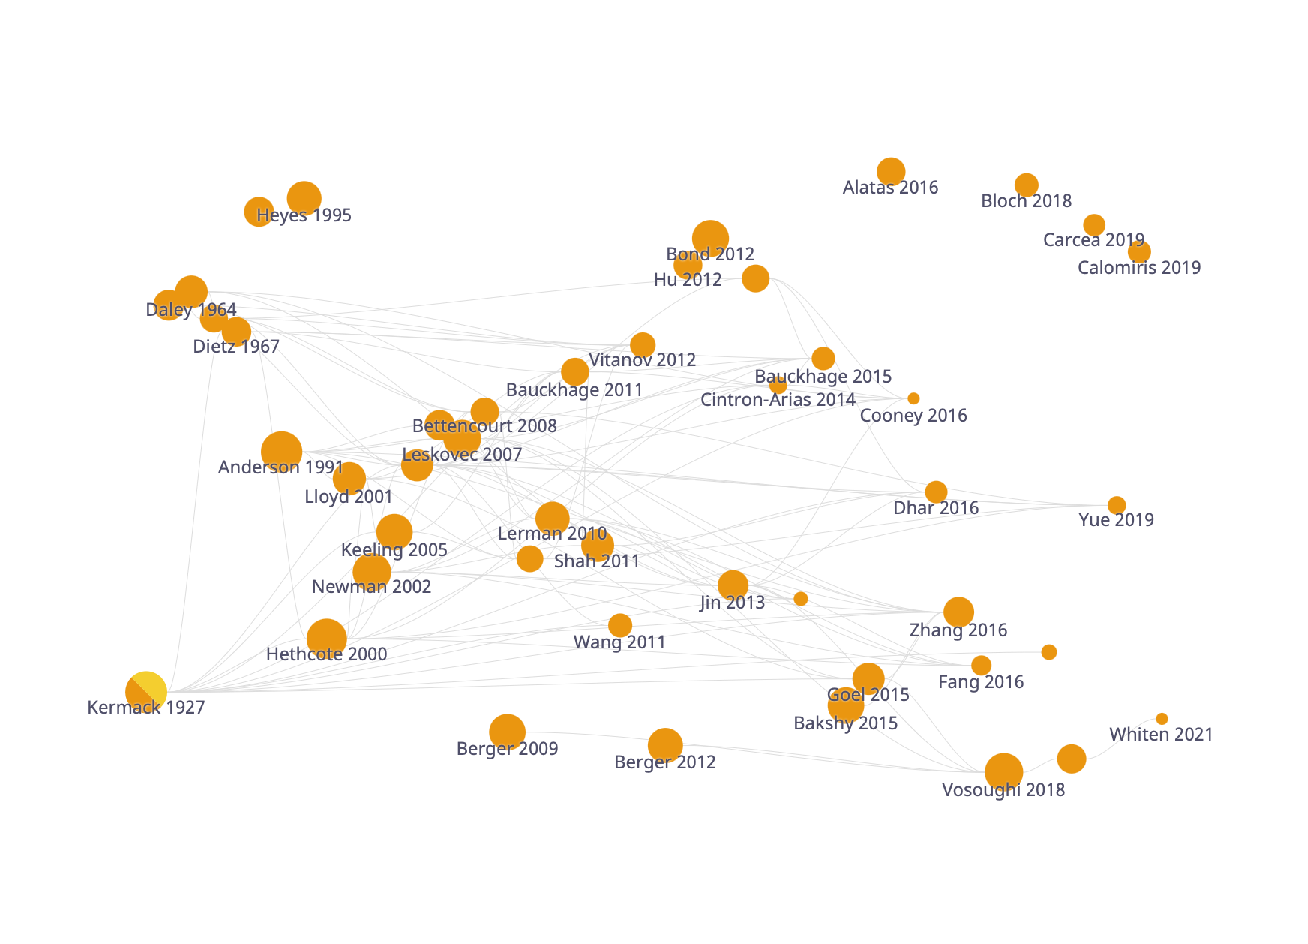
\includegraphics[width=\textwidth]{./figures/graph_other}
    \begin{flushleft}{\footnotesize Note: This graph includes selective non-economic research surveyed in this chapter, including epidemiological models of rumor/news/online content/scientific ideas. See \href{https://app.litmaps.co/shared/07C0B3F0-B4A9-4627-923C-857F1ABFD2D3}{here} for its interactive version.}
    \end{flushleft}
  \end{figure}
}

\cite{daley1964epidemics}'s proposal that rumors spread like diseases spurred a literature exploring variants of the classical epidemiological model.  A highly cited example (\cite{jin2013epidemiological}) \ifInBook{}{augments the usual three compartments of Susceptible, Infected, and Exposed with another compartment of skeptics, and}
estimates a model using the diffusion patterns of news about eight real events among Twitter users, including the Boston marathon bombings  and the resignation of Pope Benedict, and rumors such as the Mayan doomsday.  In each case, the model matches the dynamics reasonably well. \ifInBook{}{(See Figure \ref{fig:news_curve}).}

% \begin{center}[Insert Figure \ref{fig
% \begin{center}[Insert Figure \ref{fig:news_curve}  here]\end{center}
\begin{verbatimwrite}{./Slides/FigureNewsCurve}
  \begin{figure}[!ht] \centering  % [h!]
    \caption{ ~Spreading of news and rumors: Jin et al (2013)}\nocite{jin2013epidemiological}
    \label{fig:news_curve}
    \centerline{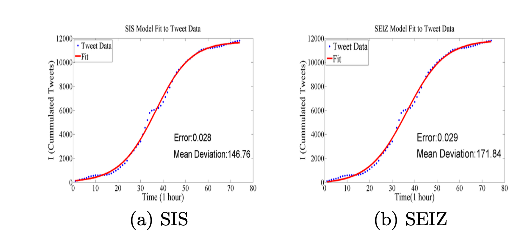
\includegraphics[width=\textwidth]{./figures/Doomsday}}
    \begin{flushleft}{\footnotesize Note: This graph is reproduced from \cite{jin2013epidemiological}, showing their fitted SIS and SEIZ model of the counts of Twitter posts related to the ``Mayan Doomsday'' rumor, which was widely circulated before December 21, 2012.}
    \end{flushleft}
  \end{figure}
\end{verbatimwrite}%%%Slides

\ifInBook{}{
  \begin{figure}[!ht] \centering  % [h!]
    \caption{ ~Spreading of news and rumors: Jin et al (2013)}\nocite{jin2013epidemiological}
    \label{fig:news_curve}
    \centerline{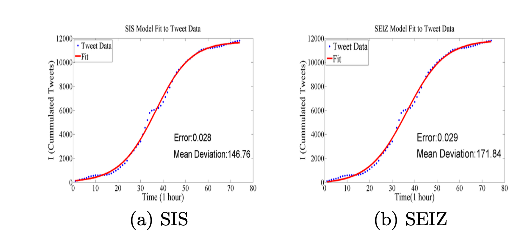
\includegraphics[width=\textwidth]{./figures/Doomsday}}
    \begin{flushleft}{\footnotesize Note: This graph is reproduced from \cite{jin2013epidemiological}, showing their fitted SIS and SEIZ model of the counts of Twitter posts related to the ``Mayan Doomsday'' rumor, which was widely circulated before December 21, 2012.}
    \end{flushleft}
  \end{figure}

}
\IfPrivate{\href{https://www.science.org/doi/10.1126/science.aap9559}{\cite{vosoughi_spread_2018}}}{\cite{vosoughi2018spread}} found that falsehood spreads on the internet faster than the truth, possibly because the interesting falsehoods have a greater capacity to produce emotional arousal.  Similarly, \IfPrivate{\href{https://journals.sagepub.com/doi/10.1509/jmr.10.0353}{\cite{berger2012makes}}}{\cite{berger2012makes}} claim that ``content that evokes high-arousal positive (awe) or negative (anger or anxiety) emotions is more viral. Content that evokes low-arousal, or deactivating, emotions (e.g., sadness) is less viral.'' \IfPrivate{\href{https://arxiv.org/abs/1805.12512}{\cite{zannettou2018origins}}}{\cite{zannettou2018origins}} found that the content of a meme affects its virality: racist and political memes are particularly viral.

\cite{kohlhasasymmetric} attempt to explain evidence that people seem to underreact to events that are not very surprising, but overreact to surprising events.  The authors attempt to model this using a combination of ideas from Sims's rational inattention framework and the Bordalo-Shleifer diagnostic expectations model, but to the extent that surprising events elicit emotional arousal, this paper may also be connected to the noneconomic literature.  %Whether or not this speculative link is correct, a broader point is that a unifying way to talk about these ideas is to characterize them all as being about ways of quantifying the degree of ``infectiousness'' of various kinds of content.

% About 126,000 rumors were spread by ∼3 million people. False news reached more people than the truth; the top 1% of false news cascades diffused to between 1000 and 100,000 people, whereas the truth rarely diffused to more than 1000 people. ...We found that false news was more novel than true news, which suggests that people were more likely to share novel information. Whereas false stories inspired fear, disgust, and surprise in replies, true stories inspired anticipation, sadness, joy, and trust. Contrary to conventional wisdom, robots accelerated the spread of true and false news at the same rate, implying that false news spreads more than the truth because humans, not robots, are more likely to spread it.

\IfPrivate{\href{https://github.com/iworld1991/EpiExp/blob/master/Literature/allcott2017social.pdf}{\cite{allcott2017social}}}{\cite{allcott2017social}} used a post-2016-election U.S.\ survey to analyze the importance of social media for fake news consumption, exposure to fake news, and partisan composition.  The paper models profit-maximizing firms who supply fake news in order to appeal to consumers subject to confirmation bias. This seems a natural extension of standard epidemiological models to incorporate the production side of the content -- ``infectiousness'' of certain ideas in subpopulations is an incentive for the production of content that will become ``viral'' because of a high reproductive number in the targeted subpopulation.

Another potential determinant of the degree to which ideas spread is explored in \IfPrivate{\href{https://www.kdd.org/exploration_files/8._CR.10.Misinformation_in_social_media_-_Final.pdf}{\cite{acemoglu2010spread}}}{\cite{acemoglu2010spread}}, who show show that the presence of ``forceful'' agents (who are immune to others' opinions) may lead to the persistence of misinformation. The key insight is that heterogeneity in infectiousness can reflect characteristics of the sender (`forcefulness') as well as the receiver.

Epidemiological models have also been effectively used to study the spread of scientific ideas.    For example,  \IfPrivate{\href{https://github.com/iworld1991/EpiExp/blob/master/Literature/bettencourt2006power.pdf}{\cite{bettencourt2006power}}}{\cite{bettencourt2006power}} find that epidemiological models perform well in explaining the the spread of Feynman diagrams through theoretical physics communities\ifInBook{.}{.}% (see Figure \ref{fig:science_ideas_curve})
 \ifInBook{}{That paper uses an SEIR model where E represents the exposed state, and a SEIZ model where Z represents skeptics (mutually exclusive with being infected) who held competing ideas. Introducing skeptics generates an additional steady state of the model where competing ideas coexist. This differs from two-compartment and three-compartment models, in which typically the system converges to a single state.}

\begin{verbatimwrite}{./Slides/FigureScienceIdeasCurve}
  \begin{figure}[!ht] \centering
    \caption{ ~Diffusion of scientific ideas: \href{http://web.mit.edu/dikaiser/www/BAKC.PhysA.pdf}{Bettencourt et al (2006)}}\nocite{bettencourt2006power}
    \label{fig:science_ideas_curve}
    \centerline{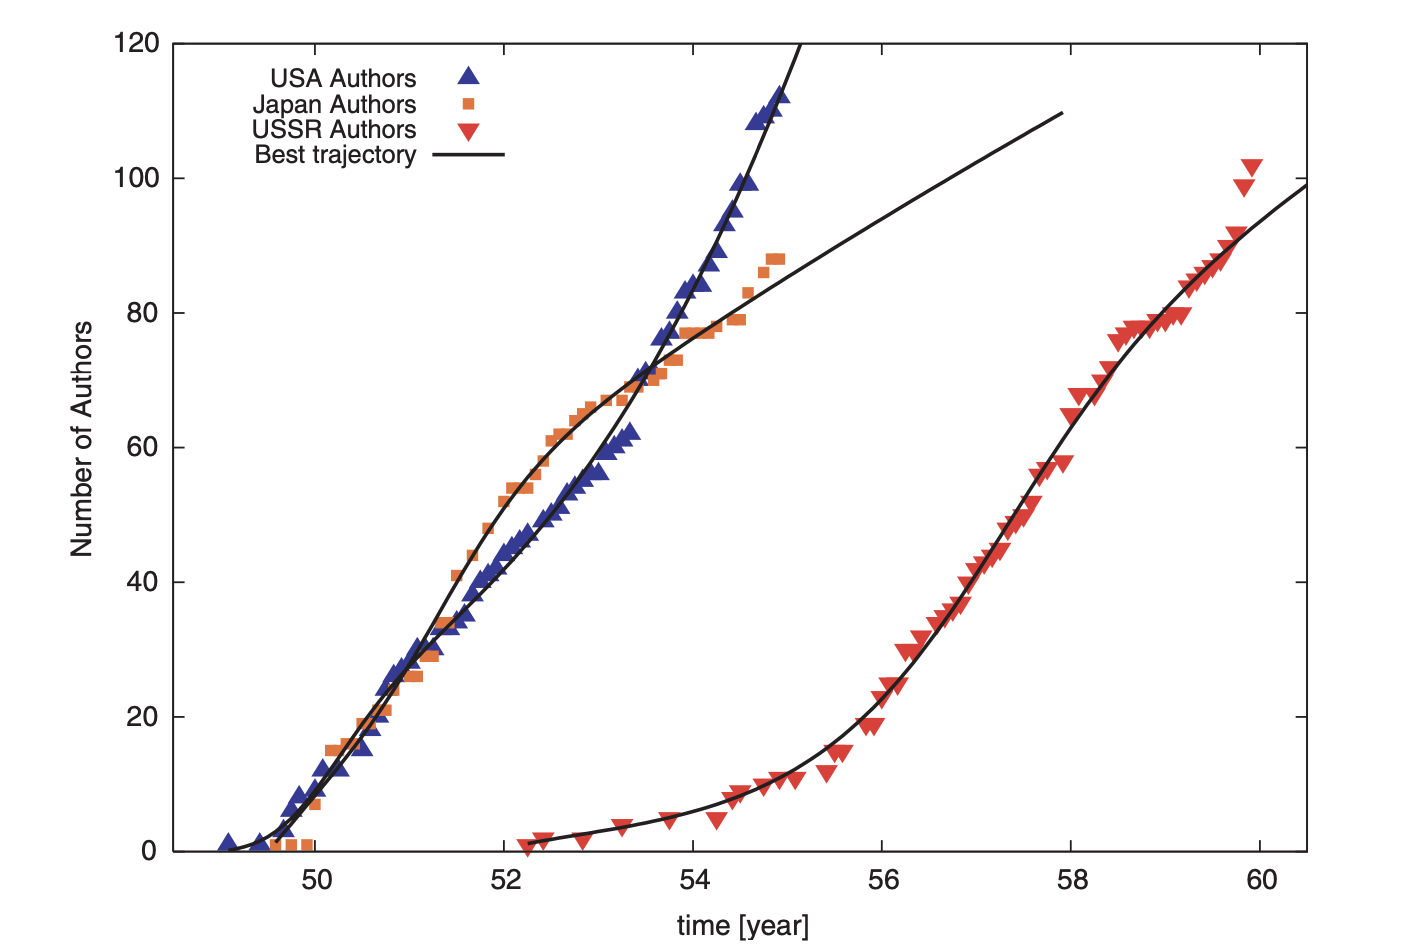
\includegraphics[width=\textwidth]{./figures/Feynman}}
    \begin{flushleft}{\footnotesize Note: \cite{bettencourt2006power}, showing their fitted SEIZ model to the diffusion dynamics of Feynman diagrams in theoretical physics communities}
    \end{flushleft}
  \end{figure}
\end{verbatimwrite}
\ifInBook{}{
}

Internet memes are a favorite topic of non-economist modelers. \IfPrivate{\href{https://github.com/iworld1991/EpiExp/blob/master/Literature/bauckhage2011insights.pdf}{\cite{bauckhage2011insights}}}{\cite{bauckhage2011insights}} shows that epidemiological models do a good job capturing the growth and decay of some famous memes.\ifInBook{}{}% (See Figure \ref{fig:memes_curve}.)}
\cite{wang2011epidemiological} finds that a modified SIR model allowing for the reinfection of the ``recovered'' fits  the propagation dynamics of various viral memes well.   A large literature has followed their work. %\href{https://github.com/iworld1991/EpiExp/blob/master/Literature/kucharski2016modelling.pdf}{\cite{kucharski2016modelling}} fits an epidemiological model to outbreaks of notable internet contagions such as the ``ice bucket challenge'' and ``no-makeup selfies.''% suggesting an initial reproduction ratio in the range of 1.9 to 2.5.

%	\href{http://cs.stanford.edu/~ashton/pubs/twiral.pdf}{\cite{goel2016structural}} explores the structural factors (independent from the intrinsic properties of the content, nature of contact process, etc.) that seem to determine whether a news story spreads more effectively from a ``broadcast'' (common-source) or from a `viral' (person-to-person) mechanism.


% Internet memes are increasingly used to sway and manipulate public opinion. This prompts the need to study their propagation, evolution, and influence across the Web. In this paper, we detect and measure the propagation of memes across multiple Web communities, using a processing pipeline based on perceptual hashing and clustering techniques, and a dataset of 160M images from 2.6B posts gathered from Twitter, Reddit, 4chan's Politically Incorrect board (/pol/), and Gab, over the course of 13 months. We group the images posted on fringe Web communities (/pol/, Gab, and The_Donald subreddit) into clusters, annotate them using meme metadata obtained from Know Your Meme, and also map images from mainstream communities (Twitter and Reddit) to the clusters. Our analysis provides an assessment of the popularity and diversity of memes in the context of each community, showing, e.g., that racist memes are extremely common in fringe Web communities. We also find a substantial number of politics-related memes on both mainstream and fringe Web communities, supporting media reports that memes might be used to enhance or harm politicians. Finally, we use Hawkes processes to model the interplay between Web communities and quantify their reciprocal influence, finding that /pol/ substantially influences the meme ecosystem with the number of memes it produces, while \td has a higher success rate in pushing them to other communities.

% There is a methodological insight for economists in these studies: To the extent that certain classes or configurations of epidemiological models are found consistently to characterize the spread of non-economic ideas (even non-textual content like videos and images), economists might be well advised to select the models that generically perform well across many kinds of content.


% \begin{center}[Insert Figure \ref{fig:memes_curve} here]\end{center}

\begin{verbatimwrite}{./Slides/FigureMemesCurve}
\begin{figure}[!ht]
  \caption{ ~Virality of internet memes: %\IfPrivate{\href{https://github.com/iworld1991/EpiExp/blob/master/Literature/bauckhage2011insights.pdf}{\cite{bauckhage2011insights}}}{\cite{bauckhage2011insights}}
  }
  \label{fig:memes_curve}
    \subfloat[``salad fingers'']{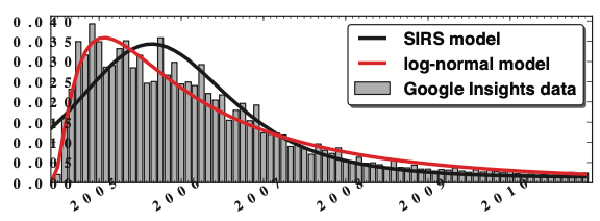
\includegraphics[width=\textwidth]{./figures/Memes1}}
    \newline
    \subfloat[``laughing baby'']{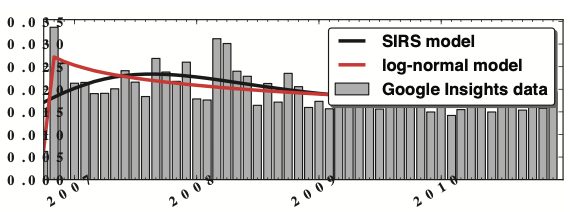
\includegraphics[width=\textwidth]{./figures/Memes2}}
    \newline
    \subfloat[``so much win'']{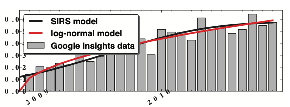
\includegraphics[width=\textwidth]{./figures/Memes3}}
    \begin{flushleft}{\footnotesize Note: This graph reproduces the SIRS model fit and log-normal fits to Google insights time series measuring the interest in six viral memes, as shown in  \cite{bauckhage2011insights}. }
    \end{flushleft}
\end{figure}

\end{verbatimwrite}
\ifInBook{}{
  {figure}[!ht] \centering \caption { ~Virality of internet memes: \href {https://github.com/iworld1991/EpiExp/blob/master/Literature/bauckhage2011insights.pdf}{\cite {bauckhage2011insights}}} \label {fig:memes_curve} \subfloat [``salad fingers'']{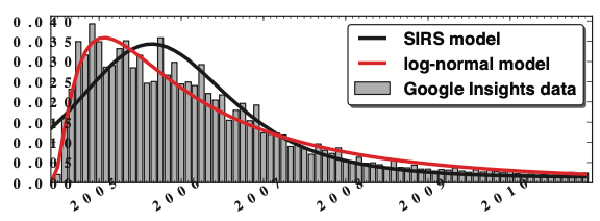
\includegraphics [width=\textwidth ]{./figures/Memes1}} \newline \subfloat [``laughing baby'']{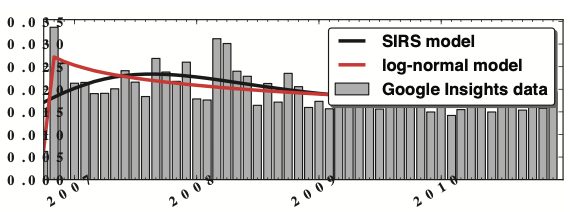
\includegraphics [width=\textwidth ]{./figures/Memes2}} \newline \subfloat [``so much win'']{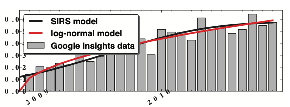
\includegraphics [width=\textwidth ]{./figures/Memes3}} \begin {flushleft}{\footnotesize Note: This graph reproduces the SIRS model fit and log-normal fits to Google insights time series measuring the interest in six viral memes, as shown in \cite {bauckhage2011insights}. } \end {flushleft} \end {figure} \end {verbatimwrite}{figure}[!ht] \centering \caption { ~Virality of internet memes: \href {https://github.com/iworld1991/EpiExp/blob/master/Literature/bauckhage2011insights.pdf}{\cite {bauckhage2011insights}}} \label {fig:memes_curve} \subfloat [``salad fingers'']{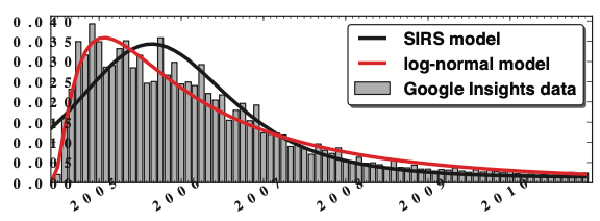
\includegraphics [width=\textwidth ]{./figures/Memes1}} \newline \subfloat [``laughing baby'']{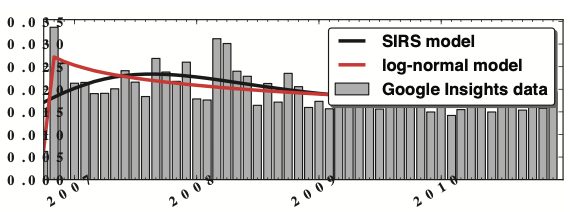
\includegraphics [width=\textwidth ]{./figures/Memes2}} \newline \subfloat [``so much win'']{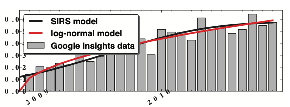
\includegraphics [width=\textwidth ]{./figures/Memes3}} \begin {flushleft}{\footnotesize Note: This graph reproduces the SIRS model fit and log-normal fits to Google insights time series measuring the interest in six viral memes, as shown in \cite {bauckhage2011insights}. } \end {flushleft} \end {figure} \end {verbatimwrite}\input {./Slides/FigureMemesCurve} 



 




  }
 % by Tao
\subsection{Future Directions}\label{subsec:future}\hypertarget{future}{}

Many suggestions for future work are contained in the foregoing.  Here, we mention a few further points that did not neatly fit above.

First, common tools from epidemiological practice could usefully be imported into expectational surveys -- particularly the deliberate efforts that epidemiologists make to determine the source of an infection (`contact tracing' being the most straightforward) -- usually by asking direct questions.  We would argue that, after a person's expectations have been elicited, at least a small amount of extra time should sometimes be allocated to asking ``why do you believe [x].''  The respondent may not be able to give an answer, but in many cases they might have a useful response: ``A friend told me'' or ``I read it in the newspaper'' or ``I did some research on the internet'' or ``I learned that from my parents when I was growing up.''\footnote{\cite{arrondel2020informative} provides an example of this approach. In a survey of French households, they not only elicited respondents' stock market expectations, but also the size and financial expertise of the social circles within which they discuss financial matters. The paper finds that social interactions affect stock market beliefs mostly through information channels, instead of social  preferences.} Any of these answers (or potentially others) might prove very helpful in narrowing the set of models that are plausible for explaining any particular set of beliefs.  Direct questions could also help distinguish between different kinds of information: A job seeker might learn from friends that job prospects have improved, which causes improved expectations. These same friends might also tell the job-seeker about a specific current vacancy.  If job seekers were directly asked separate questions about expectations and vacancy tips, it would be much easier to distinguish a mechanism in which optimistic job-seekers work harder to find jobs from a mechanism in which job vacancy tips are more frequent in periods when optimism is greater.

Above, we made mention of several kinds of evidence that information from some sources, or of some kinds, was more infectious.  The literature on homophily, for example, suggests that ideas spread more readily among persons who have more in common.  And even among social connections with otherwise-similar characteristics, some are likely to be more credible than others.  %({\it ceteris paribus}, stock advice from an investment banker cousin might be more likely to be trusted than from his identical twin who is a circus acrobat.)
Direct survey questions asking respondents which sources of information they find most persuasive, and why, might prove very helpful in thinking about the most appropriate structure for our models (and potentially even addressing problems like the Manski's reflection problem.)

Epidemiological ideas might also prove to be useful in understanding how to interpret results like those in \cite{galesic2018asking}, who find that election surveys that ask participants about the voting intentions of their social contacts proved more accurate in predicting voting outcomes than surveys asking people how they themselves would vote, and other results that suggest that it is easier to elicit prevalence of socially stigmatized behaviors or attitudes by asking respondents about prevalence among members of their social circles rather than asking the respondent about themselves.  (``Are you a racist'' does not elicit useful responses - and may even result in the termination of the survey; ``how many of your friends would you say might be racist'' seems to generate much more revealing responses; cf \cite{radas2021predicted}.)

\hypertarget{subsec:literature}{}

\subsection{Literature Summation}\label{subsec:literature}

\ifthenelse{\boolean{inBook}}{}{We have barely scratched the surface of the scholarly literature with interesting evidence about the ways in which social interactions shape population beliefs.  Even within economics, where the topic has received less attention than might be expected, there is so much material that we are confident that we have missed some content that should have been included, for which we hereby preemptively apologize to readers (and authors).}% and would encourage the authors of such work bring it to our attention.

Ideas that we would term `epidemiological' have emerged independently in scholarly fields who (ironically) seem largely unaware of each others' existence.  Different terminology and methodological tools have developed for ideas that are close cousins; this likely has hindered the ability of participants in distant fields to recognize deep commonalities in their work.

For example, the work on ``social learning'' in macroeconomics studies the propagation of competing forecasting rules via agent interactions in simulated populations.  If it were couched as being about the spread of beliefs in the efficacy of the rules, this work would have satisfied our criteria that it addressed a substantive economic question using a mechanism by which beliefs were transmitted by social interaction.  But authors in this literature often do not describe their models in explicitly epidemiological terms, nor do they typically propose testing their models by querying simulated agents about their expectations, and comparing simulated expectations data to actual expectations data.

Nor does this work take much notice of Shiller's longstanding view that economic dynamics reflect the competition of `narratives' that `go viral.'  ``Social learning'' models'  forecasting rules are arguably exactly how one might want to make a computational representation of what Shiller calls a narrative, and the economic dynamics that result from the increasing prevalence of the rules that succeed in `tournaments' are a good candidate for a computational representation of the consequences of what might be meant by the claim that `narratives' can `go viral.'

\ifthenelse{\boolean{inBook}}{}{
  Reciprocally, it does not seem that scholars interested in the ``narrative approach'' have embraced ``social learning in macroeconomics'' literature -- maybe because papers in that literature usually do not describe the decisions the agents make as being a consequence of the ``narratives'' they have adopted to understand the world.
}

One of our ambitions is for this survey to infect scholars with the idea that it is useful to describe their models in a common language drawn as much as possible from the familiar domains of epidemiological modeling and network theory:  Infectiousness, susceptibility, transmissibility, exposure, immunity, mixing, homophily, reproduction rates, degree distributions, clustering, and so on (in addition to whatever domain-specific terminology may be natural to their particular topic).

\section{Conclusion}

\label{conclusion}%\hyperref{conclusion}{}

Many of the obstacles, real and perceived, to the construction of what we call full-fledged Epidemiological Expectations models have lessened over the last two decades.

A large body of evidence now finds that opinions on economic questions are sharply heterogeneous, and that people's choices are related to their opinions.

Data from social networks now provide the possibility of directly observing the key mechanisms of the social transmission of ideas -- as  has already been done in a few cases of economic models (and many cases outside of economics).  Other work, based not on social network data but on measures like geographical proximity or shared workplaces or common places of origin, has found evidence of social transmission of ideas, while another strand of research has explored the ways in which news outlets can be modeled as a source of heterogeneity in beliefs if news stories have degrees of either exposure or infectiousness less than 100 percent.

The recent successes achieved by the HA-Macro literature from the incorporation of realistic heterogeneity in non-expectational variables seem likely to tempt scholars to see what more can be accomplished with structural models of expectational heterogeneity calibrated to match empirically measured expectations.  While there are other mechanisms for generating such heterogeneity, epidemiological modeling is a promising candidate.

An epidemiological expectations modeling approach is by no means applicable only to macroeconomic questions -- expectations are at the heart of all sorts of economic questions.  But available tools allow economists to expand their imagination far beyond the limited `classical' epidemiological models.  A particularly attractive direction that any literature written by economists is likely to take is to apply the discipline's sophisticated tools for analyzing purposive behavior, as is done for example in the paper by~\cite{lucas2014knowledge} whose agents optimally expose themselves to the possibility of infection with new ideas in the hopes of improving their productivity -- something scholars have done since time immemorial.

% (and outside it -- we have deliberately avoided dipping our toes into the vast literature on ``viral marketing'' -- for that see \cite{watts2007viral}).

\begin{comment}
\begin{itemize}
	\item Future directions of research
	\begin{itemize}
		\item Better measurements of market expectations/beliefs that could be fit into epi models.
		\begin{itemize}
			\item Explicitly eliciting people's source of information and reasons for held beliefs could shed light on the role of social connections on expectation formation.
		\end{itemize}
		\item Integrating observed social structure and interpersonal interactions with belief surveys to identify the epi models of expectations.
		\item Incorporating epi models of expectations into structural/general equilibrium models to examine if the belief dynamics has important implications for aggregate dynamics and outcomes
	\end{itemize}
\end{itemize}
\end{comment}




% \newpage
% \section*{Figures}


\begin{verbatimwrite}{./Slides/FigureParker}%%%Slides
\begin{figure}[!ht] \centering  % [h!]
	\caption{ ~Portfolio responses to 2016 U.S. election}
	\label{fig:parker}
	\centerline{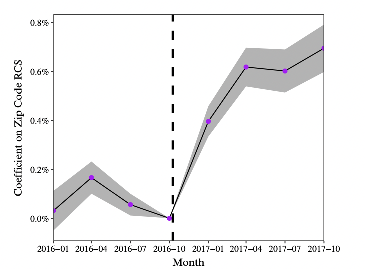
\includegraphics[width=\textwidth]{./figures/parker.png}}
	\begin{flushleft}
		{\footnotesize Note: reproduced from \cite{meeuwis2018belief}, this figure reports the baseline regression coefficients of equity share on zip-code level  campaign contribution share to Republican candidate for the three quarters prior to the election and the four quarters following the election, relative to allocations just before the election.}
	\end{flushleft}
\end{figure}
\end{verbatimwrite}%%%Slides
%%%Slides
  \begin{figure}[!ht] \centering  % [h!]
    \caption{ ~Portfolio responses to 2016 U.S. election}
    \label{fig:parker}
    \centerline{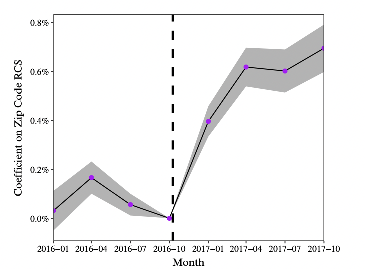
\includegraphics[width=\textwidth]{./figures/parker}}
    \begin{flushleft}
      {\footnotesize Note: reproduced from \cite{meeuwis2018belief}, this figure reports the baseline regression coefficients of equity share on zip-code level  campaign contribution share to Republican candidate for the three quarters prior to the election and the four quarters following the election, relative to allocations just before the election.}
    \end{flushleft}
  \end{figure}
%%%Slides



\begin{verbatimwrite}{./Slides/FigureSIRFlowDiagram}%%%Slides
\begin{figure}[!ht] \centering  % [h!]
	\caption{ ~A SIR model of stock investors}
		\label{fig:sir_diagram}
		\centerline{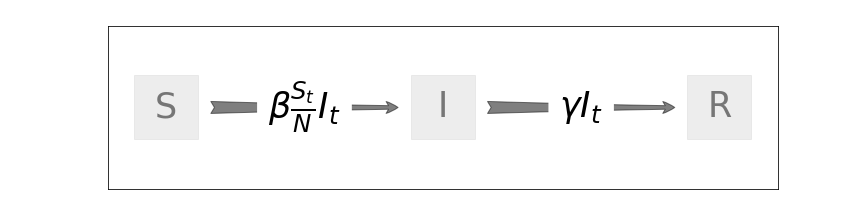
\includegraphics[width=\textwidth]{./figures/flow_diagram.png}}
		\begin{flushleft}
		{\footnotesize Note: This graph plots the transitions between different compartments in the SIR model of the stock investors as described in \cite{shiller1989survey}. }
			\end{flushleft}
	\end{figure}
\end{verbatimwrite}%%%Slides
%%%Slides
	\begin{figure}[!ht] \centering  % [h!]
		\caption{ ~A SIR model of stock investors}
		\label{fig:sir_diagram}
		\centerline{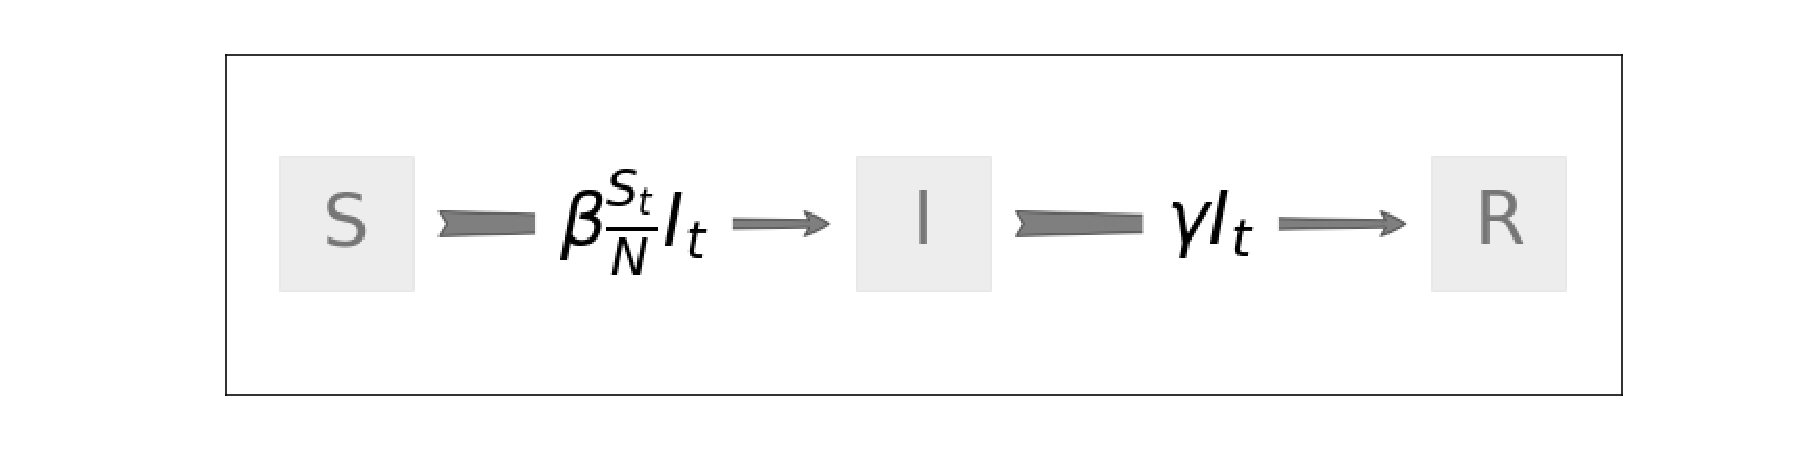
\includegraphics[width=1.5\textwidth]{./figures/flow_diagram}}
		\begin{flushleft}
			{\footnotesize Note: This graph plots the transitions between different compartments in the SIR model of stock investors described in \cite{shiller1989survey}. }
		\end{flushleft}
	\end{figure}


\newpage

\begin{verbatimwrite}{./Slides/FigureSIRSimulation}%%%Slides
\begin{figure}[!ht] \centering  % [h!]
	\caption{ ~Simulated dynamics from a SIR model of stock investors}
	\label{fig:sir_simulate}
	\centerline{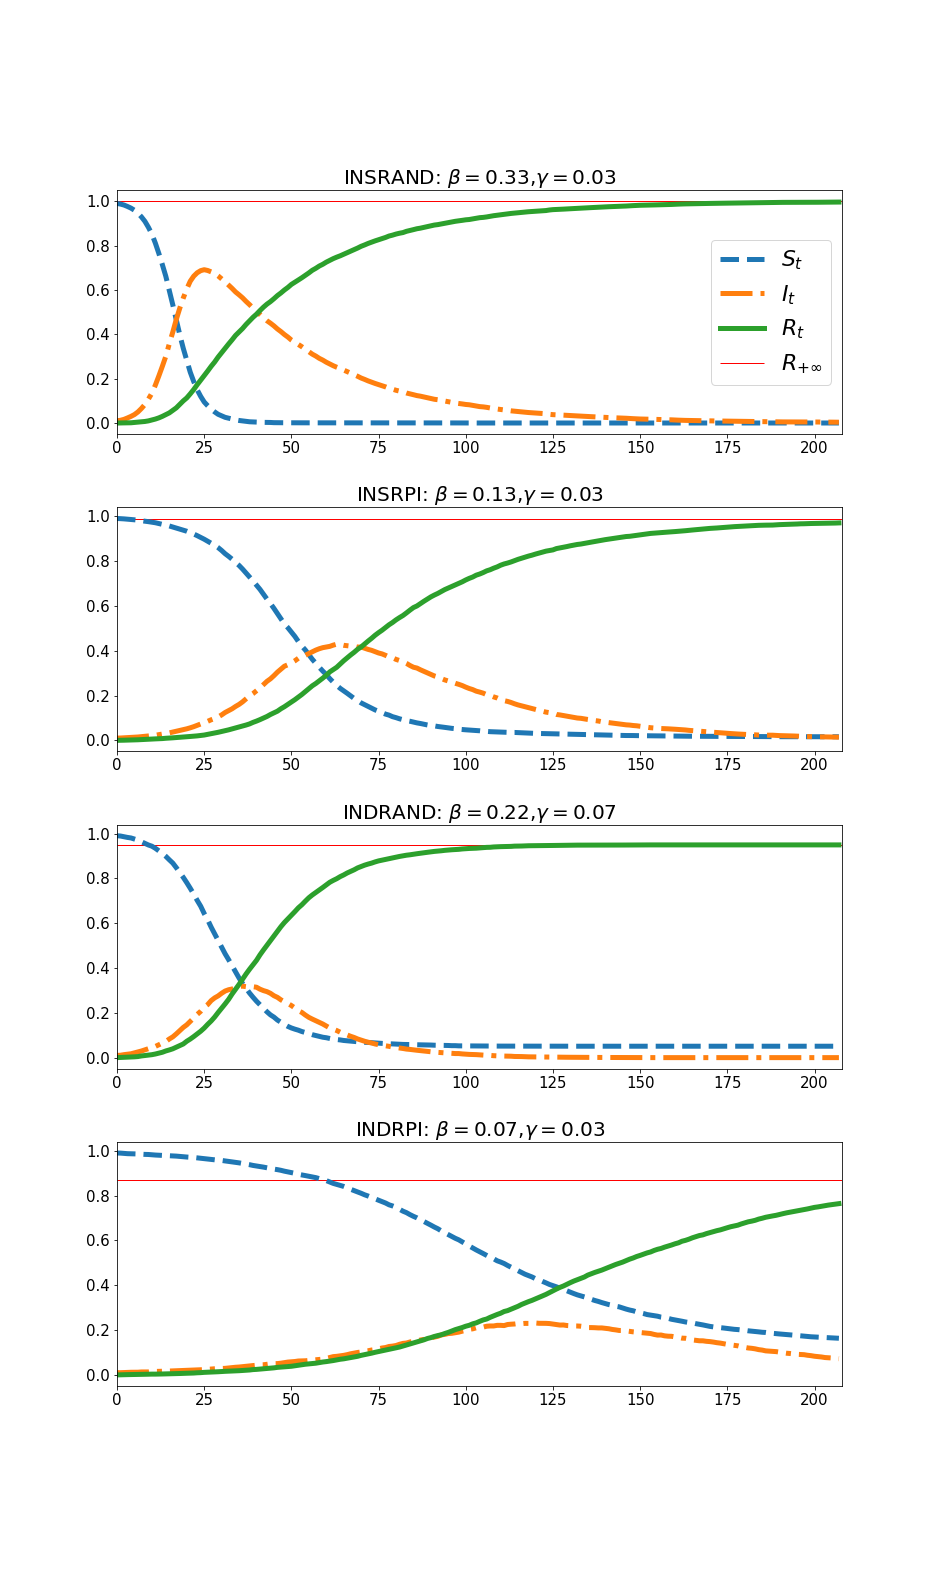
\includegraphics[width=0.7\textwidth]{./figures/sir_simulate.png}}
	\begin{flushleft}
	{\footnotesize Note: This graph plots the simulated paths of populations in different compartments in a SIR model of stock investors, as described in \cite{shiller1989survey}. We use the median estimates of the infection rate $\beta$ and recovery rate $\gamma$ for four samples: institutional investors for a randomly selected stock (INSRAND), institutional investors for a rapidly rising stock (INSRPI), individual investors for a random stock (INDRAND), and individual investors for a rapidly rising stock (INDRPI). The horizontal dashed line corresponds to the limiting size of compartment of $R$ in the long run. The simulation is done with the Python library ``NDlib'', for details, see the companion \href{https://github.com/llorracc/EpiExp/blob/master/SIR_Ndlib.ipynb}{Jupyter Notebook}. }
				\end{flushleft}
\end{figure}
\end{verbatimwrite}%%%Slides
%%%Slides
  \begin{figure} \centering  % [h!]  [!ht]
    \caption{ ~Simulated dynamics from an SIR model of stock investors}
    \label{fig:sir_simulate}
    \centerline{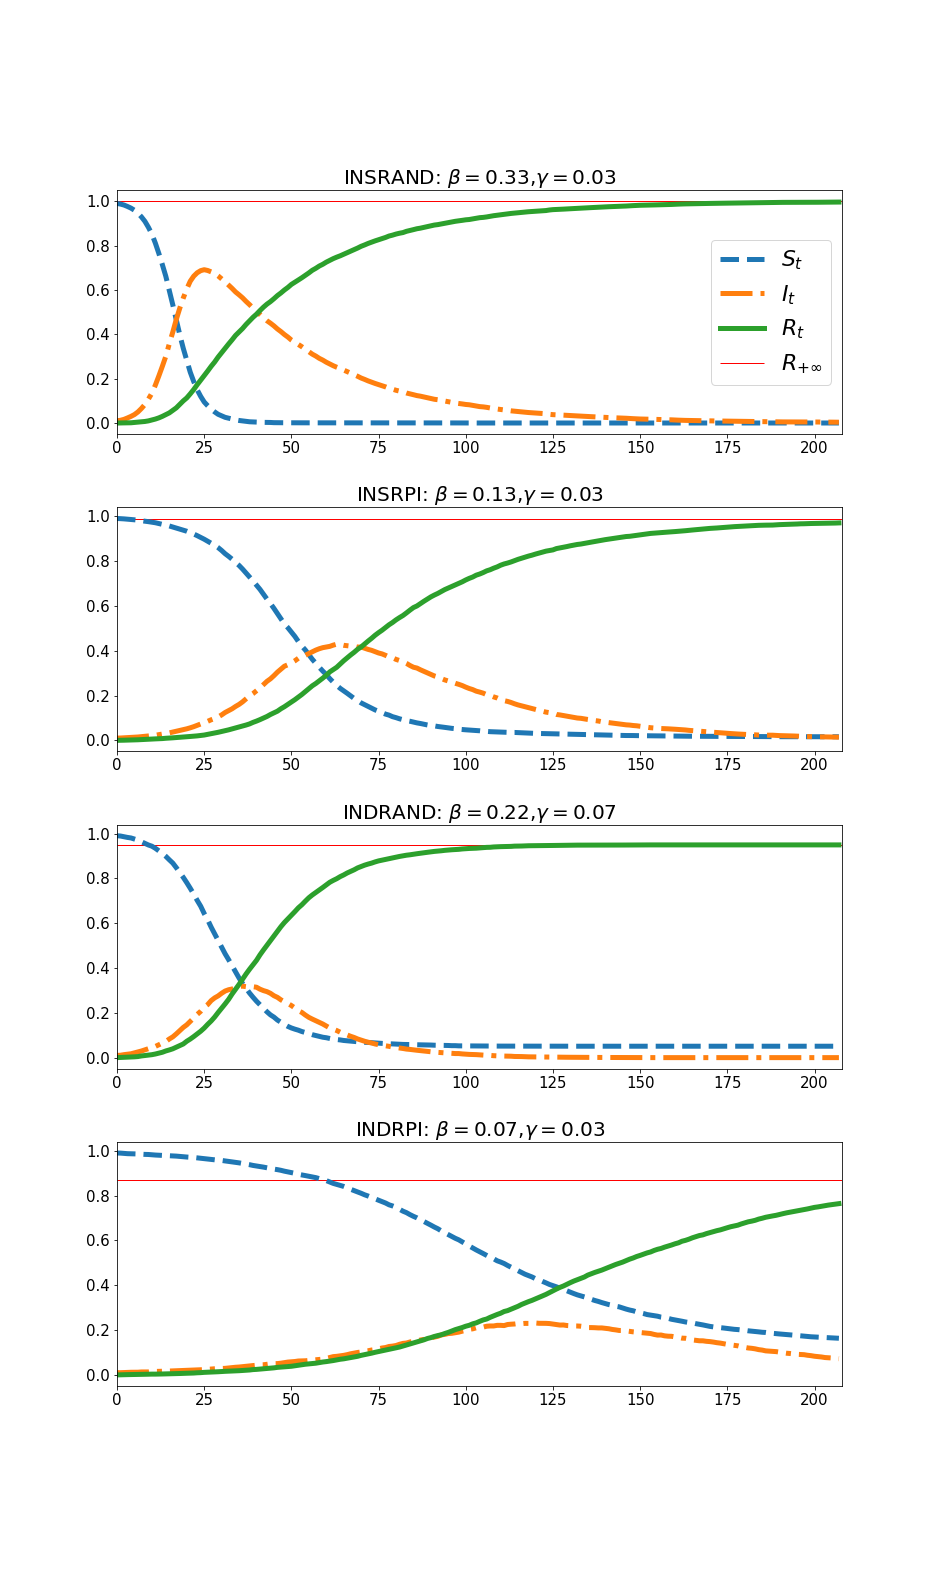
\includegraphics[width=0.85\textwidth,height=0.85\textheight]{./figures/sir_simulate}}
    \begin{flushleft}
      {\footnotesize Note: This graph plots the simulated paths of populations in different compartments in a SIR model of stock investors, as described in \cite{shiller1989survey}. We use the median estimates of the infection rate $\beta$ and recovery rate $\gamma$ for four samples: institutional investors for a randomly selected stock (INSRAND), institutional investors for a rapidly rising stock (INSRPI), individual investors for a random stock (INDRAND), and individual investors for a rapidly rising stock (INDRPI). The horizontal thin solid line corresponds to the limiting size of compartment of $R$ in the long run. The simulation is done with the Python library \href{https://ndlib.readthedocs.io/en/latest/}{``NDlib''}, for details, see the companion \href{https://github.com/llorracc/EpiExp/blob/master/SIR_Ndlib.ipynb}{Jupyter Notebook}. }
    \end{flushleft}
  \end{figure}
%%%Slides

\newpage

\begin{figure}[!ht] \centering  % [h!]
	\caption{ ~Literature map of cited papers}
	\label{fig:graph_mixer}
	\centerline{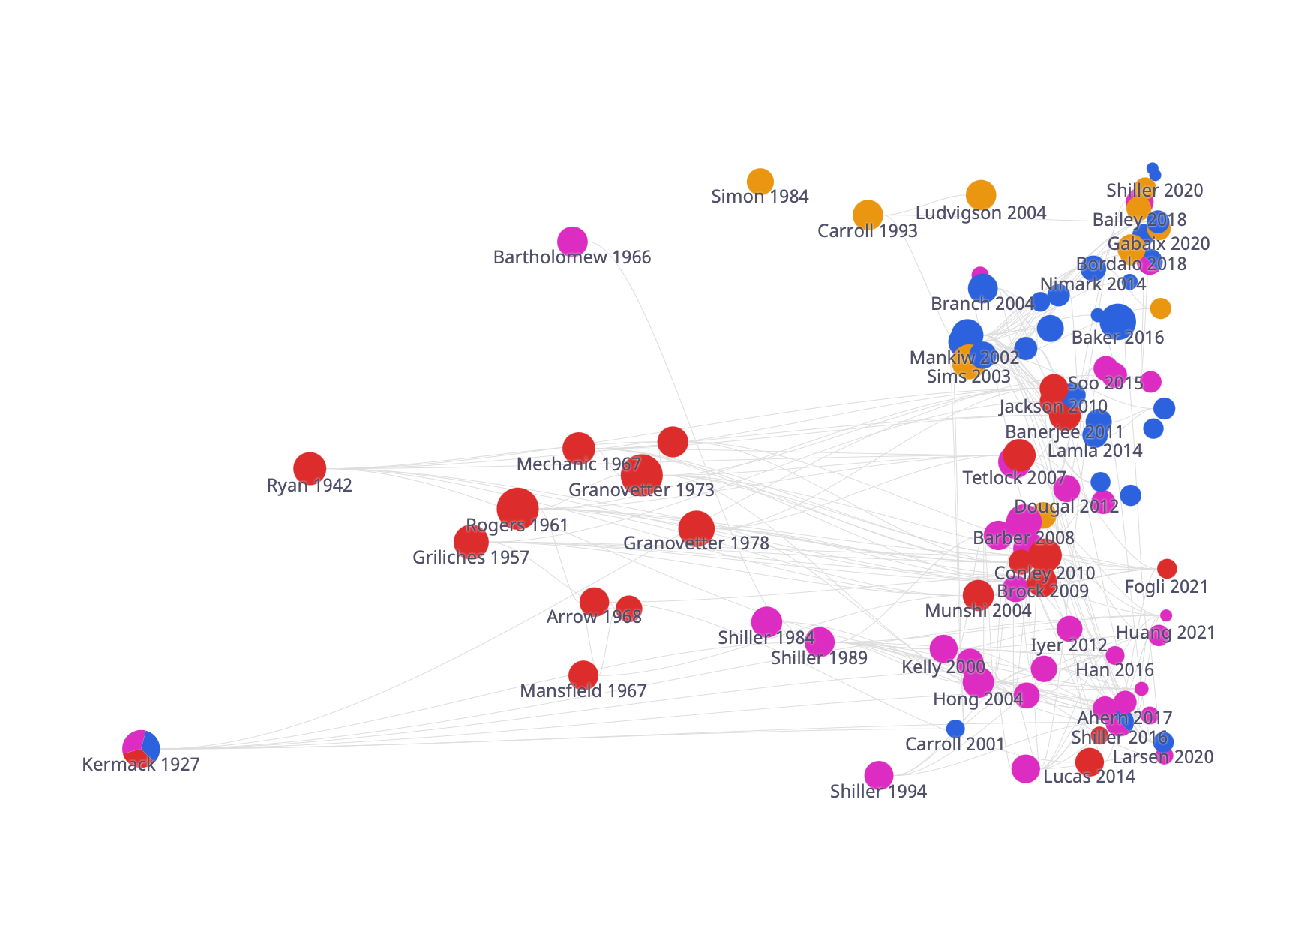
\includegraphics[width=\textwidth]{./figures/graph_mixer}}
	\begin{flushleft}
		{\footnotesize Note: This graph includes selected papers under three topics of epidemiological expectations: technological diffusion, asset market investment and macroeconomic expectations, represented by different color.  It also includes other papers we have cited because they have results likely to be interesing to EE modelers.}
	\end{flushleft}
\end{figure}

\newpage

\begin{figure}[!ht] \centering  % [h!]
	\caption{ ~Literature map of EE models of technological diffusion}
	\label{fig:graph_diffusion}
	\centerline{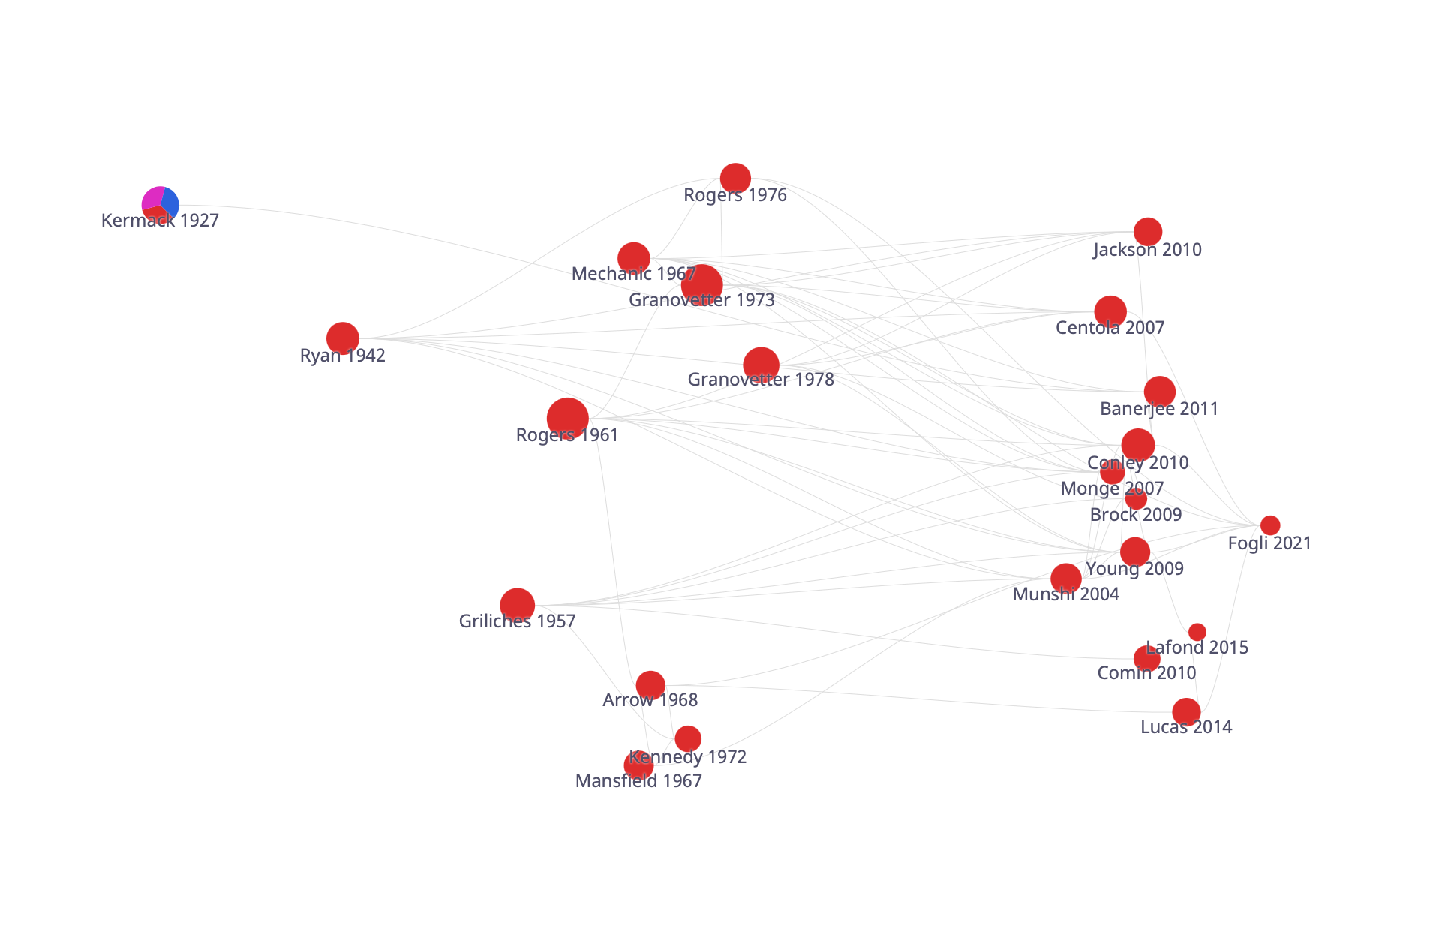
\includegraphics[width=\textwidth]{./figures/graph_diffusion}}
		\begin{flushleft}
{\footnotesize Note: This graph includes selected papers under the topic of epidemiological modeling of technological/innovation diffusion in economics and its related literature from other fields. See \href{https://app.litmaps.co/shared/1D9003CB-75FE-4633-B60A-79B70E03B691}{here} for its interactive version.}
				\end{flushleft}
\end{figure}

\newpage

\begin{figure}[!ht] \centering  % [h!]
	\caption{ ~Literature map of EE models of stock/housing market investment}
	\label{fig:graph_investment}
	\centerline{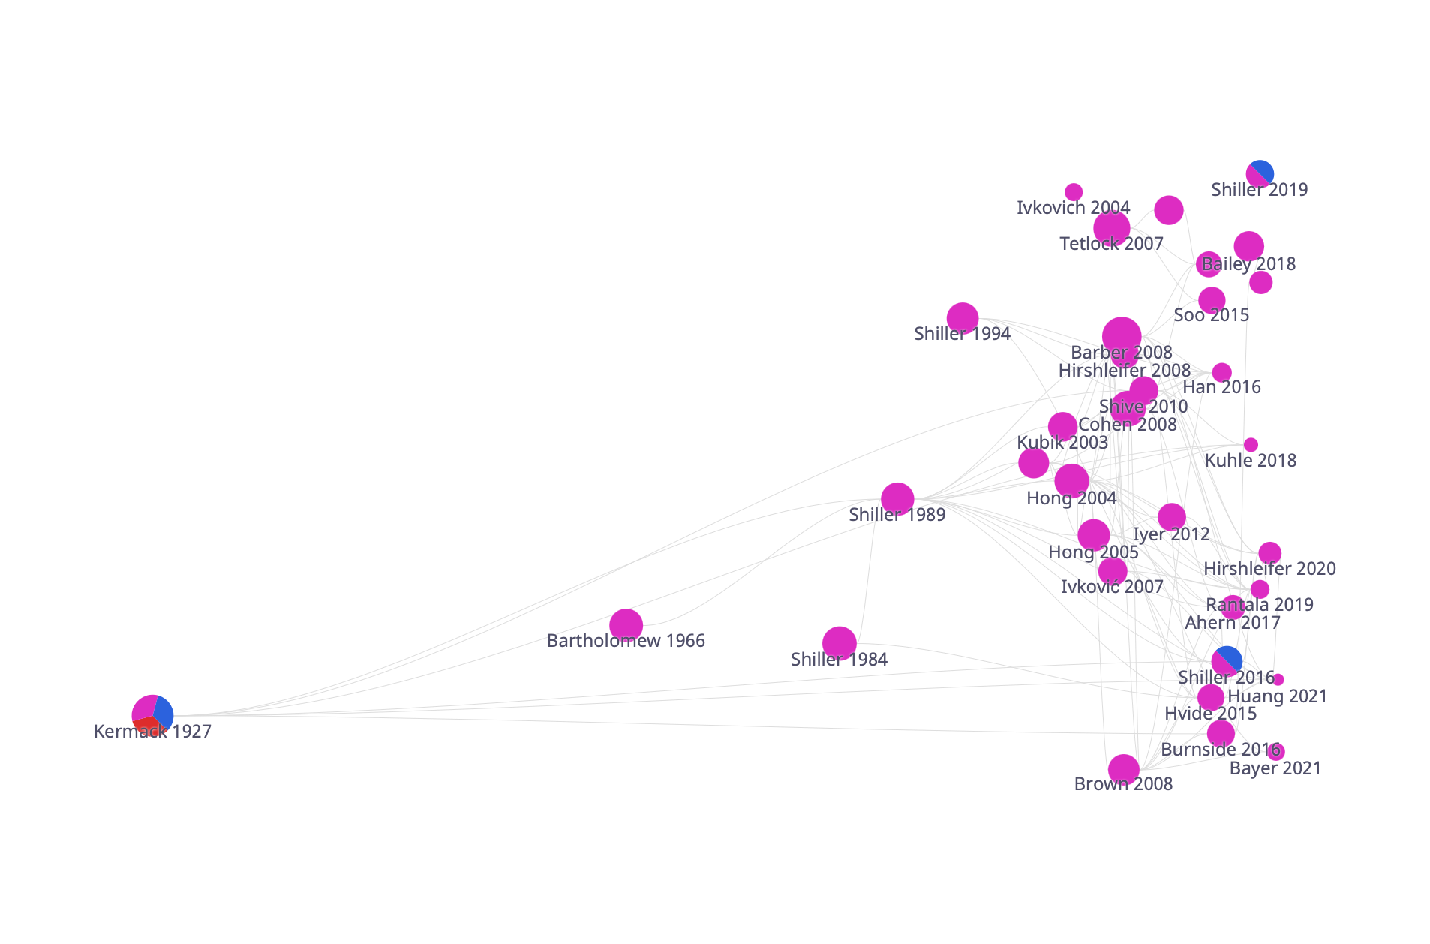
\includegraphics[width=\textwidth]{./figures/graph_investment}}
			\begin{flushleft}
	{\footnotesize Note: This graph includes selected papers related to epidemiological models of expectations in financial markets such as stocks and housing, and studies on the role of news media in financial markets. See \href{https://app.litmaps.co/shared/E25276CA-8725-437B-8241-11961EFB3FB4}{here} for its interactive version.}
					\end{flushleft}
\end{figure}

\newpage


\begin{figure}[!ht] \centering  % [h!]
    %\hypertarget{graphmacro}{}
		\caption{ ~Literature map of EE models of macroeconomic expectations}
	\label{fig:graph_macro}
	\centerline{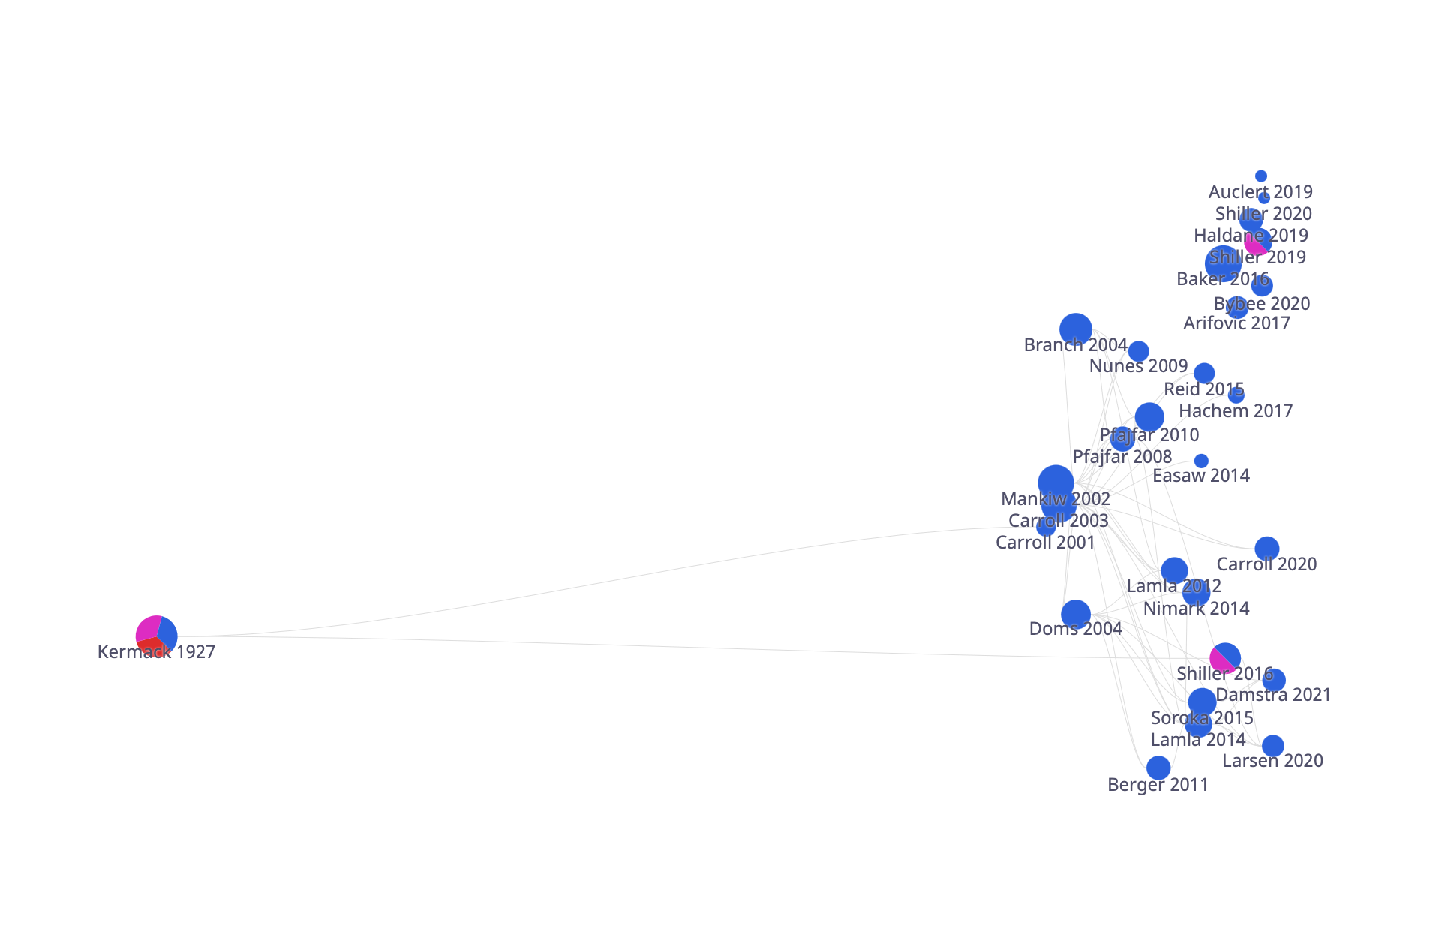
\includegraphics[width=\textwidth]{./figures/graph_macro}}
				\begin{flushleft}
		{\footnotesize Note: This graph includes selected papers related to epidemiological models of macroeconomic expectations, and research on the interaction between news media and macroeconomic expectations. See \href{https://app.litmaps.co/shared/289F57F4-FDE5-4F94-B1A9-2BA7419DB719}{here} for its interactive version.}
							\end{flushleft}
\end{figure}

\newpage

\begin{figure}[!ht] \centering  % [h!]
	\caption{ ~Other fields related to epidemiological models}
	\label{fig:graph_other}
	\centerline{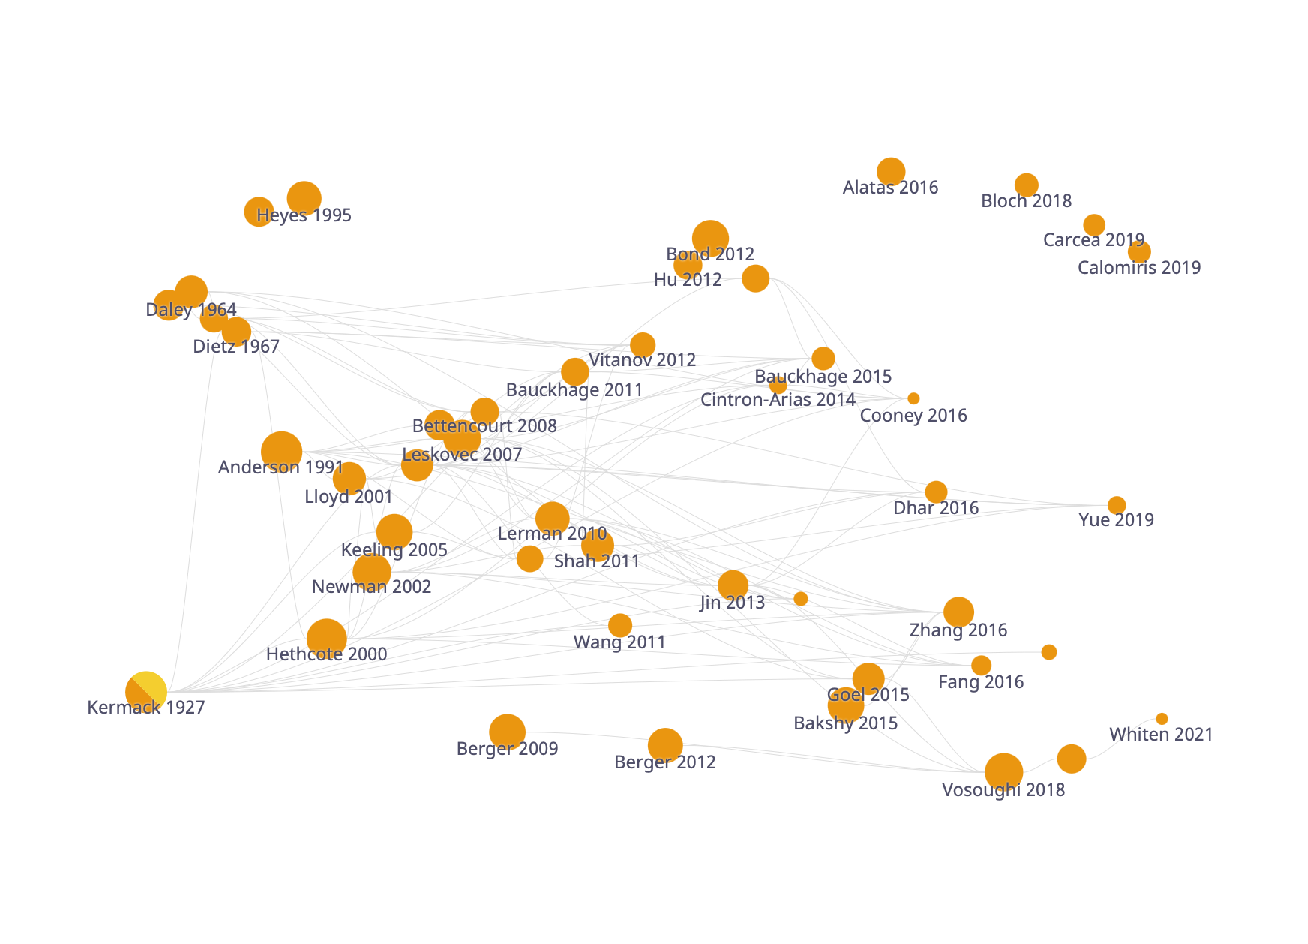
\includegraphics[width=\textwidth]{./figures/graph_other}}
				\begin{flushleft}{\footnotesize Note: This graph includes all other papers surveyed in this chapter. It includes epi models of rumor/news/online content/scientific ideas as well as other economic research on bank runs, herd behaviors, contagion, and peer effects. See \href{https://app.litmaps.co/shared/B5FA1F14-01A8-4C9D-BF23-BE0F62293FAF}{here} for its interactive version.}
						\end{flushleft}
\end{figure}


\newpage


\begin{verbatimwrite}{./Slides/FigureNewsCurve}
\begin{figure}[!ht] \centering  % [h!]
	\caption{ ~Spreading of news and rumors: \href{https://people.cs.vt.edu/ramakris/papers/news-rumor-epi-snakdd13.pdf}{\cite{jin2013epidemiological}}}
	\label{fig:news_curve}
	\centerline{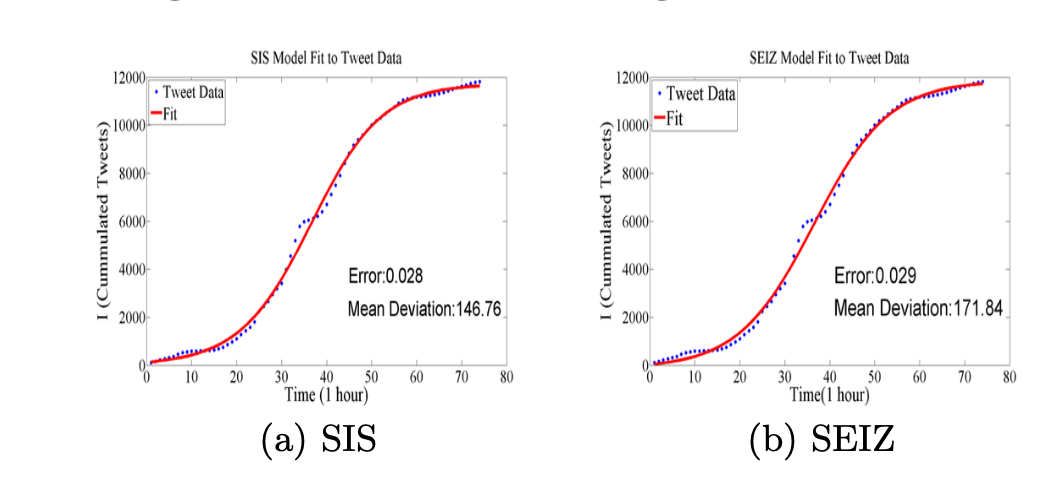
\includegraphics[width=\textwidth]{./figures/Doomsday.png}}
		\begin{flushleft}{\footnotesize Note: This graph is reproduced from \cite{jin2013epidemiological}, showing their fitted SIS and SEIZ model of the counts of Twitter posts related to the ``Doomsday'' rumor, which was widely circulated before December 21, 2012.}
	\end{flushleft}
\end{figure}
\end{verbatimwrite}%%%Slides
  \begin{figure}[!ht] \centering  % [h!]
    \caption{ ~Spreading of news and rumors: Jin et al (2013)}\nocite{jin2013epidemiological}
    \label{fig:news_curve}
    \centerline{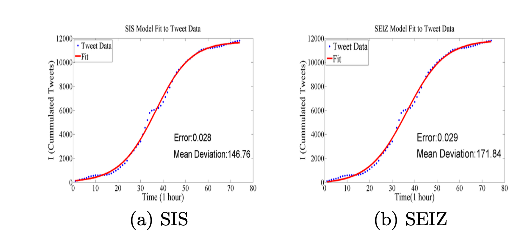
\includegraphics[width=\textwidth]{./figures/Doomsday}}
    \begin{flushleft}{\footnotesize Note: This graph is reproduced from \cite{jin2013epidemiological}, showing their fitted SIS and SEIZ model of the counts of Twitter posts related to the ``Mayan Doomsday'' rumor, which was widely circulated before December 21, 2012.}
    \end{flushleft}
  \end{figure}


\newpage


\begin{verbatimwrite}{./Slides/FigureScienceIdeasCurve}
\begin{figure}[!ht] \centering  % [h!]
	\caption{ ~Diffusion of scientific ideas: \href{http://web.mit.edu/dikaiser/www/BAKC.PhysA.pdf}{\cite{bettencourt2006power}}}
	\label{fig:science_ideas_curve}
	\centerline{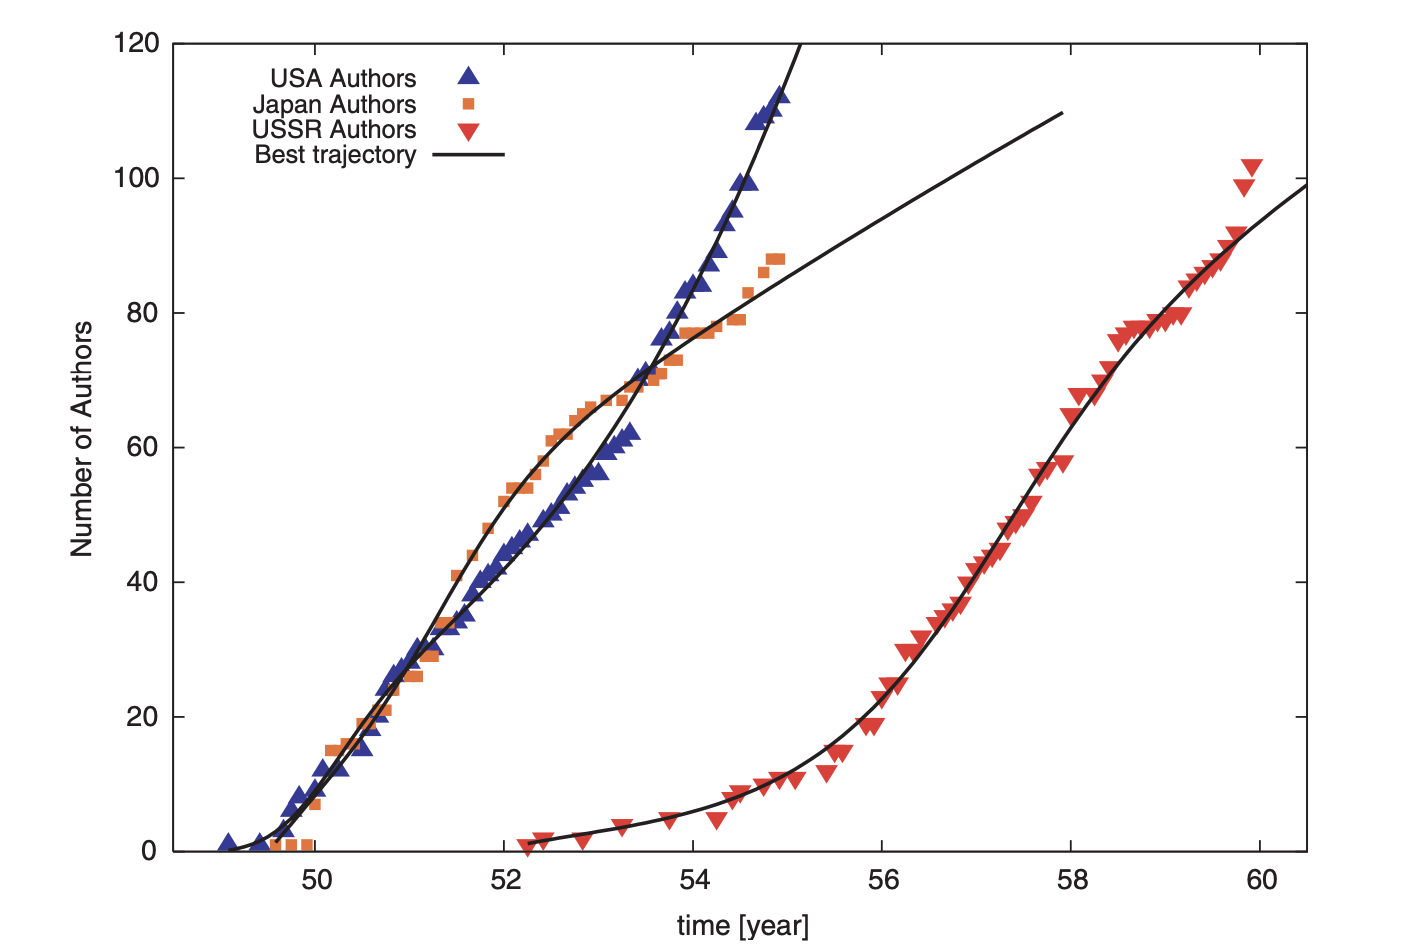
\includegraphics[width=\textwidth]{./figures/Feynman.png}}
		\begin{flushleft}{\footnotesize Note: This graph is reproduced from \cite{bettencourt2006power}, showing their fitted SEIZ model to the diffusion dynamics of Feynman diagrams in three theoretical physics communities, measured by the cumulative number of authors using the Feynman diagrams.}
	\end{flushleft}
\end{figure}
\end{verbatimwrite}%%%Slides
	\begin{figure}[!ht] \centering  % [h!]
		\caption{ ~Diffusion of scientific ideas: \href{http://web.mit.edu/dikaiser/www/BAKC.PhysA.pdf}{Bettencourt et al (2006)}}\nocite{bettencourt2006power}
		\label{fig:science_ideas_curve}
		\centerline{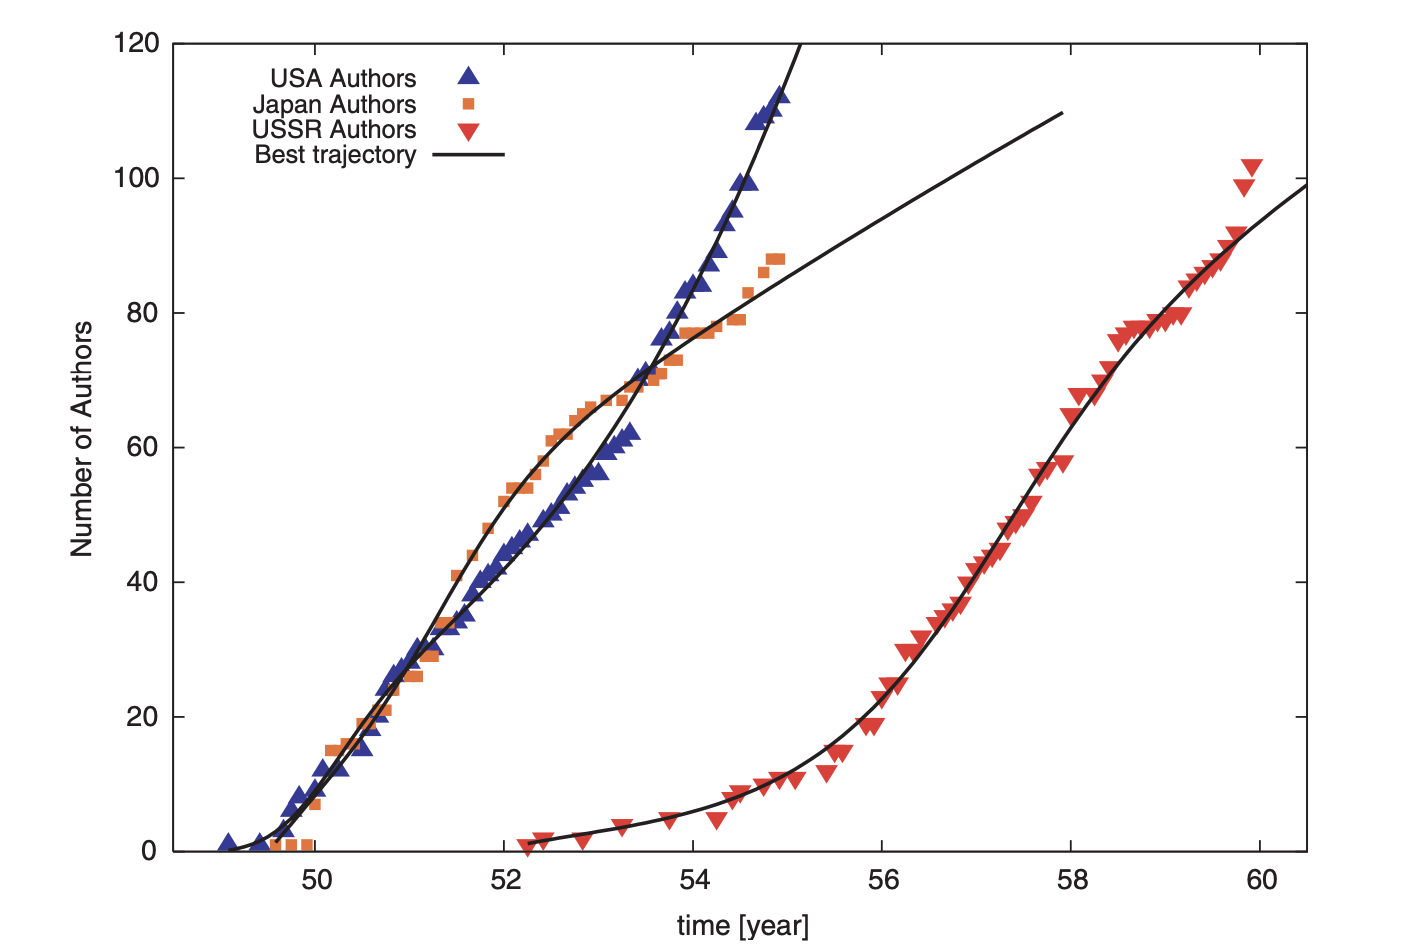
\includegraphics[width=\textwidth]{./figures/Feynman}}
		\begin{flushleft}{\footnotesize Note: This graph is reproduced from \cite{bettencourt2006power}, showing their fitted SEIZ model to the diffusion dynamics of Feynman diagrams in three theoretical physics communities, measured by the cumulative number of authors using the Feynman diagrams.}
		\end{flushleft}
	\end{figure}


\newpage

\begin{verbatimwrite}{./Slides/FigureMemesCurve}
\begin{figure}[!ht] \centering  % [h!]
	\caption{ ~Virality of internet memes: \href{https://github.com/iworld1991/EpiExp/blob/master/Literature/bauckhage2011insights.pdf}{\cite{bauckhage2011insights}}}
	\label{fig:memes_curve}
	\centerline{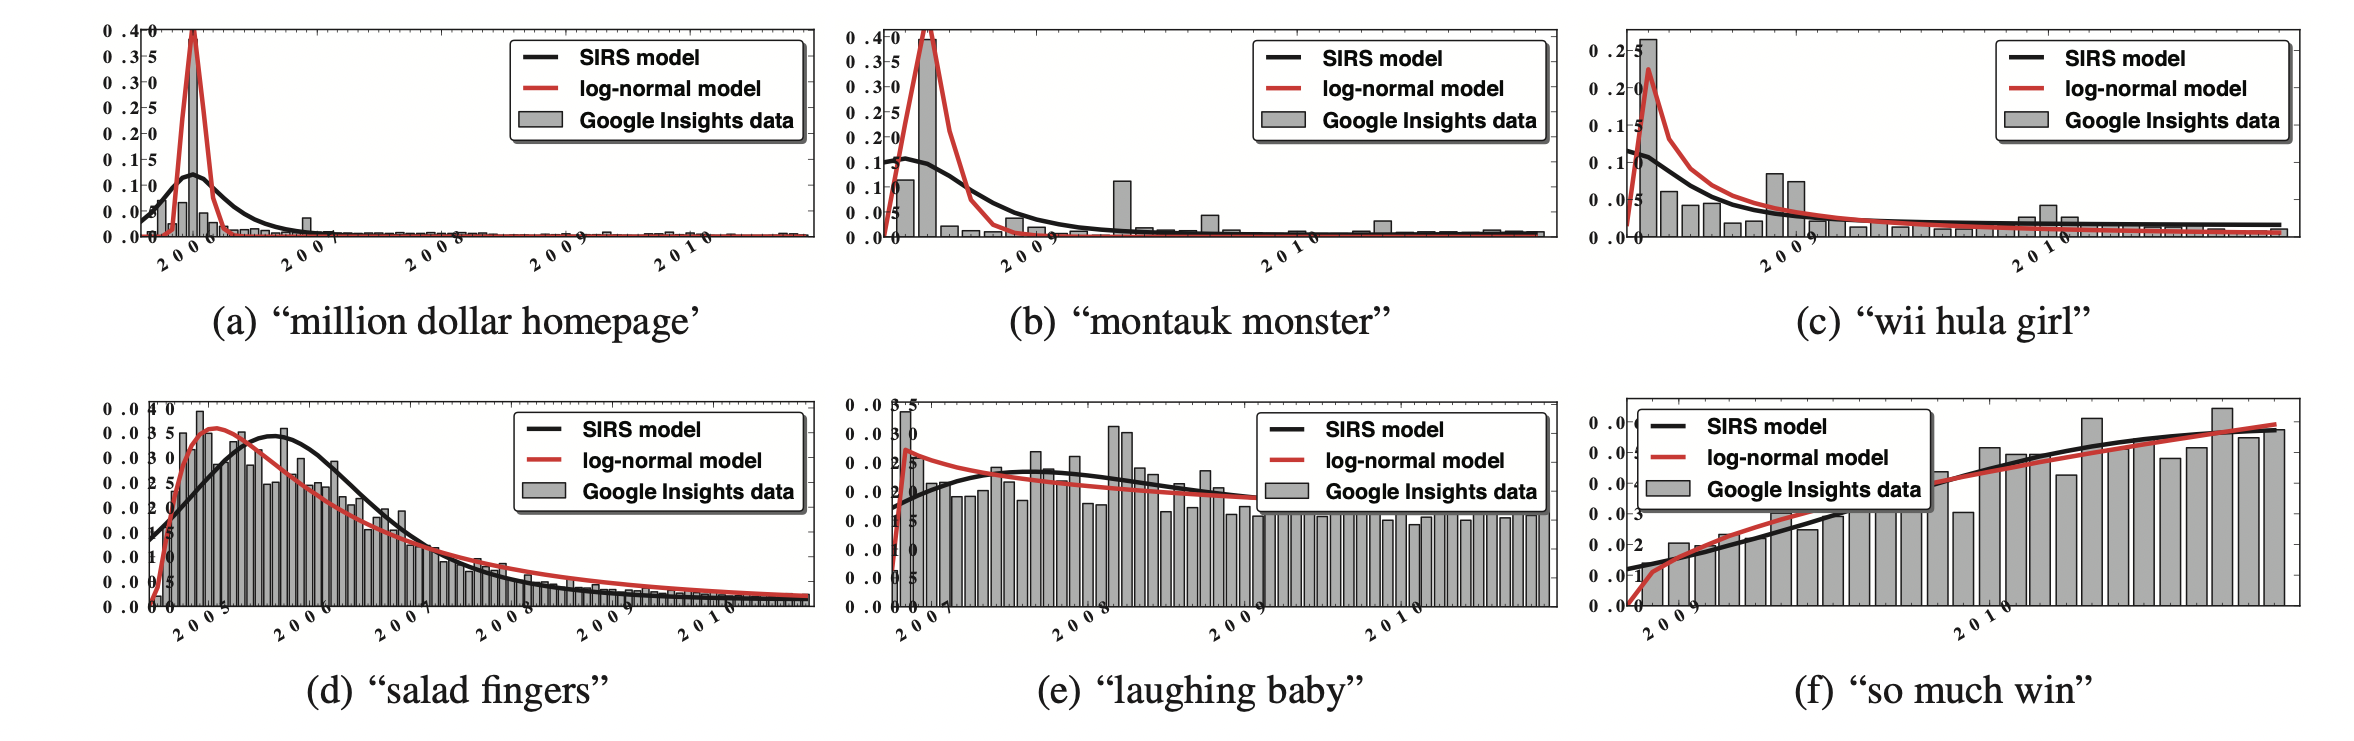
\includegraphics[width=\textwidth]{./figures/Memes.png}}
	\begin{flushleft}{\footnotesize Note: This graph reproduces the SIRS model fit and log-normal fits to Google insights time series measuring the interest in six viral memes, as shown in  \cite{bauckhage2011insights}. }
\end{flushleft}
\end{figure}
\end{verbatimwrite}%%%Slides
{figure}[!ht] \centering \caption { ~Virality of internet memes: \href {https://github.com/iworld1991/EpiExp/blob/master/Literature/bauckhage2011insights.pdf}{\cite {bauckhage2011insights}}} \label {fig:memes_curve} \subfloat [``salad fingers'']{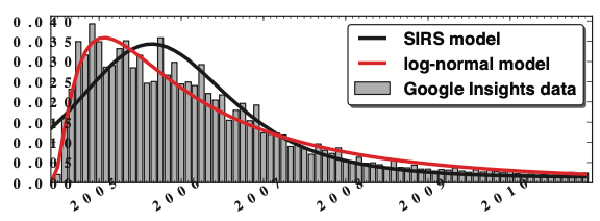
\includegraphics [width=\textwidth ]{./figures/Memes1}} \newline \subfloat [``laughing baby'']{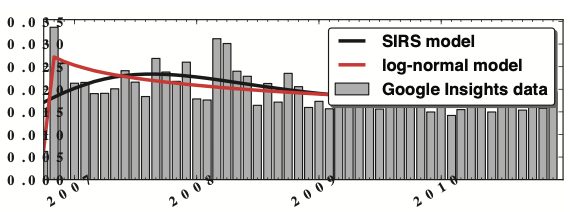
\includegraphics [width=\textwidth ]{./figures/Memes2}} \newline \subfloat [``so much win'']{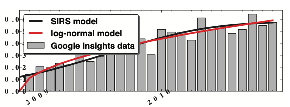
\includegraphics [width=\textwidth ]{./figures/Memes3}} \begin {flushleft}{\footnotesize Note: This graph reproduces the SIRS model fit and log-normal fits to Google insights time series measuring the interest in six viral memes, as shown in \cite {bauckhage2011insights}. } \end {flushleft} \end {figure} \end {verbatimwrite}{figure}[!ht] \centering \caption { ~Virality of internet memes: \href {https://github.com/iworld1991/EpiExp/blob/master/Literature/bauckhage2011insights.pdf}{\cite {bauckhage2011insights}}} \label {fig:memes_curve} \subfloat [``salad fingers'']{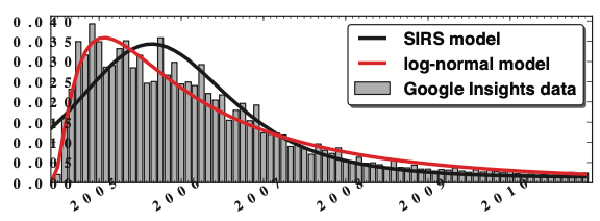
\includegraphics [width=\textwidth ]{./figures/Memes1}} \newline \subfloat [``laughing baby'']{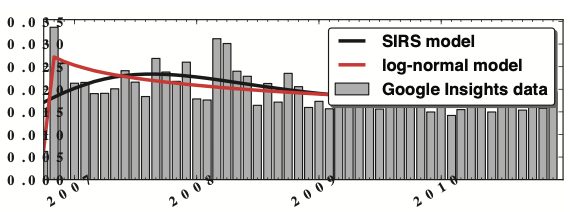
\includegraphics [width=\textwidth ]{./figures/Memes2}} \newline \subfloat [``so much win'']{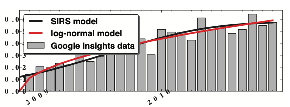
\includegraphics [width=\textwidth ]{./figures/Memes3}} \begin {flushleft}{\footnotesize Note: This graph reproduces the SIRS model fit and log-normal fits to Google insights time series measuring the interest in six viral memes, as shown in \cite {bauckhage2011insights}. } \end {flushleft} \end {figure} \end {verbatimwrite}\input {./Slides/FigureMemesCurve} 



 






% \clearpage\vfill\eject


\addcontentsline{toc}{section}{References}
\ifthenelse{\boolean{inBook}}{
  \bibliographystyle{apalike}
  \pagebreak
  \bibliography{reference,handbook}
}{\pagebreak\bibliography{reference,handbook}}
% \bibliographystyle{Vancouver-Numbered-Style(3)}

\pagebreak

